%\usepackage{latex8}
\documentclass[final]{IEEEtran}
%\documentclass[conference]{IEEEtran}
%\documentclass[10pt]{article}
%%%%%%%%%%%%%%%%%%%%%%%%%%%%%%%%%%%%%%%%%%%%%%%%%%%%%%%%%%%%%%%%%%%%%%%%%%%%%%%%%%%%%%%%%%%%%%%%%%%%%%%%%%%%%%%%%%%%%%%%%%%%
\usepackage{url}
\usepackage{amssymb}
\usepackage{times}
\usepackage[dvips]{graphicx}
\usepackage{lscape,moreverb,latexsym,graphics,makeidx}
\usepackage{amsmath}
\usepackage{color}
\usepackage{isabelle}
\usepackage{isabellesym}
\usepackage{longtable}

\setcounter{MaxMatrixCols}{10}
%TCIDATA{OutputFilter=LATEX.DLL}
%TCIDATA{Version=4.00.0.2312}
%TCIDATA{LastRevised=Wednesday, April 13, 2011 10:51:04}
%TCIDATA{<META NAME="GraphicsSave" CONTENT="32">}

\newtheorem{theorem}{Theorem}
\newtheorem{acknowledgement}[theorem]{Acknowledgement}
\newtheorem{algorithm}[theorem]{Algorithm}
\newtheorem{axiom}[theorem]{Axiom}
\newtheorem{case}[theorem]{Case}
\newtheorem{claim}[theorem]{Claim}
\newtheorem{conclusion}[theorem]{Conclusion}
\newtheorem{condition}[theorem]{Condition}
\newtheorem{conjecture}[theorem]{Conjecture}
\newtheorem{corollary}[theorem]{Corollary}
\newtheorem{criterion}[theorem]{Criterion}
\newtheorem{definition}[theorem]{Definition}
\newtheorem{example}[theorem]{Example}
\newtheorem{exercise}[theorem]{Exercise}
\newtheorem{lemma}[theorem]{Lemma}
\newtheorem{notation}[theorem]{Notation}
\newtheorem{problem}[theorem]{Problem}
\newtheorem{proposition}[theorem]{Proposition}
\newtheorem{remark}[theorem]{Remark}
\newtheorem{solution}[theorem]{Solution}
\newtheorem{summary}[theorem]{Summary}
\newenvironment{proof}[1][Proof]{\noindent\textbf{#1.} }{\ \rule{0.5em}{0.5em}}
%\newlength{\fminilength}
%\newsavebox{\fminibox}
%\newenvironment{fmini}[1][\linewidth]
 % {\setlength{\fminilength}{#1\fboxsep-2\fboxrule}   \vspace{2ex}\noindent\begin{lrbox}{\fminibox}\begin{minipage}{\fminilength}   \mbox{ }\hfill\vspace{-2.5ex}}  {\end{minipage}\end{lrbox}\vspace{1ex}\hspace{0ex}   \framebox{\usebox{\fminibox}}}
%\newenvironment{specification}
%{\noindent\tt\begin{fmini}\begin{tabbing}X\=X12345\=XXXX\=XXXX\=XXXX\=XXXX\=XXXX
%\=\+\kill} {\end{tabbing}\normalfont\end{fmini}}

\newlength{\fminilength}
\newsavebox{\fminibox}
\newenvironment{fmini}[1][\linewidth]
  {\setlength{\fminilength}{#1\fboxsep-2\fboxrule}%
   \vspace{2ex}\noindent\begin{lrbox}{\fminibox}\begin{minipage}{\fminilength}%
   \mbox{ }\hfill\vspace{-2.5ex}}%
  {\end{minipage}\end{lrbox}\vspace{1ex}\hspace{0ex}%
   \framebox{\usebox{\fminibox}}}

\newenvironment{specification}
{\noindent\footnotesize\tt\begin{fmini}\begin{tabbing}X\=X12345\=XXXX\=XXXX\=XXXX\=XXXX\=XXXX
\=\+\kill} {\end{tabbing}\normalfont\end{fmini}}


  \def\|#1|{\mathid{#1}}
    \newcommand{\mathid}[1]{\ensuremath{\mathit{#1}}}
   % \<name> or \codeid{name} denotes computer code identifiers
   \def\<#1>{\codeid{#1}}   \newcommand{\codeid}[1]{\ifmmode{\mbox{\ttfamily{#1}}}\else{\ttfamily #1}\fi}
%% Macros for Scientific Word 2.5 documents saved with the LaTeX filter.
%Copyright (C) 1994-95 TCI Software Research, Inc.
\typeout{TCILATEX Macros for Scientific Word 2.5 <22 Dec 95>.}
\typeout{NOTICE:  This macro file is NOT proprietary and may be 
freely copied and distributed.}
%
\makeatletter
%
%%%%%%%%%%%%%%%%%%%%%%
% macros for time
\newcount\@hour\newcount\@minute\chardef\@x10\chardef\@xv60
\def\tcitime{
\def\@time{%
  \@minute\time\@hour\@minute\divide\@hour\@xv
  \ifnum\@hour<\@x 0\fi\the\@hour:%
  \multiply\@hour\@xv\advance\@minute-\@hour
  \ifnum\@minute<\@x 0\fi\the\@minute
  }}%

%%%%%%%%%%%%%%%%%%%%%%
% macro for hyperref
\@ifundefined{hyperref}{\def\hyperref#1#2#3#4{#2\ref{#4}#3}}{}

% macro for external program call
\@ifundefined{qExtProgCall}{\def\qExtProgCall#1#2#3#4#5#6{\relax}}{}
%%%%%%%%%%%%%%%%%%%%%%
%
% macros for graphics
%
\def\FILENAME#1{#1}%
%
\def\QCTOpt[#1]#2{%
  \def\QCTOptB{#1}
  \def\QCTOptA{#2}
}
\def\QCTNOpt#1{%
  \def\QCTOptA{#1}
  \let\QCTOptB\empty
}
\def\Qct{%
  \@ifnextchar[{%
    \QCTOpt}{\QCTNOpt}
}
\def\QCBOpt[#1]#2{%
  \def\QCBOptB{#1}
  \def\QCBOptA{#2}
}
\def\QCBNOpt#1{%
  \def\QCBOptA{#1}
  \let\QCBOptB\empty
}
\def\Qcb{%
  \@ifnextchar[{%
    \QCBOpt}{\QCBNOpt}
}
\def\PrepCapArgs{%
  \ifx\QCBOptA\empty
    \ifx\QCTOptA\empty
      {}%
    \else
      \ifx\QCTOptB\empty
        {\QCTOptA}%
      \else
        [\QCTOptB]{\QCTOptA}%
      \fi
    \fi
  \else
    \ifx\QCBOptA\empty
      {}%
    \else
      \ifx\QCBOptB\empty
        {\QCBOptA}%
      \else
        [\QCBOptB]{\QCBOptA}%
      \fi
    \fi
  \fi
}
\newcount\GRAPHICSTYPE
%\GRAPHICSTYPE 0 is for TurboTeX
%\GRAPHICSTYPE 1 is for DVIWindo (PostScript)
%%%(removed)%\GRAPHICSTYPE 2 is for psfig (PostScript)
\GRAPHICSTYPE=\z@
\def\GRAPHICSPS#1{%
 \ifcase\GRAPHICSTYPE%\GRAPHICSTYPE=0
   \special{ps: #1}%
 \or%\GRAPHICSTYPE=1
   \special{language "PS", include "#1"}%
%%%\or%\GRAPHICSTYPE=2
%%%  #1%
 \fi
}%
%
\def\GRAPHICSHP#1{\special{include #1}}%
%
% \graffile{ body }                                  %#1
%          { contentswidth (scalar)  }               %#2
%          { contentsheight (scalar) }               %#3
%          { vertical shift when in-line (scalar) }  %#4
\def\graffile#1#2#3#4{%
%%% \ifnum\GRAPHICSTYPE=\tw@
%%%  %Following if using psfig
%%%  \@ifundefined{psfig}{\input psfig.tex}{}%
%%%  \psfig{file=#1, height=#3, width=#2}%
%%% \else
  %Following for all others
  % JCS - added BOXTHEFRAME, see below
    \leavevmode
    \raise -#4 \BOXTHEFRAME{%
        \hbox to #2{\raise #3\hbox to #2{\null #1\hfil}}}%
}%
%
% A box for drafts
\def\draftbox#1#2#3#4{%
 \leavevmode\raise -#4 \hbox{%
  \frame{\rlap{\protect\tiny #1}\hbox to #2%
   {\vrule height#3 width\z@ depth\z@\hfil}%
  }%
 }%
}%
%
\newcount\draft
\draft=\z@
\let\nographics=\draft
\newif\ifwasdraft
\wasdraftfalse

%  \GRAPHIC{ body }                                  %#1
%          { draft name }                            %#2
%          { contentswidth (scalar)  }               %#3
%          { contentsheight (scalar) }               %#4
%          { vertical shift when in-line (scalar) }  %#5
\def\GRAPHIC#1#2#3#4#5{%
 \ifnum\draft=\@ne\draftbox{#2}{#3}{#4}{#5}%
  \else\graffile{#1}{#3}{#4}{#5}%
  \fi
 }%
%
\def\addtoLaTeXparams#1{%
    \edef\LaTeXparams{\LaTeXparams #1}}%
%
% JCS -  added a switch BoxFrame that can 
% be set by including X in the frame params.
% If set a box is drawn around the frame.

\newif\ifBoxFrame \BoxFramefalse
\newif\ifOverFrame \OverFramefalse
\newif\ifUnderFrame \UnderFramefalse

\def\BOXTHEFRAME#1{%
   \hbox{%
      \ifBoxFrame
         \frame{#1}%
      \else
         {#1}%
      \fi
   }%
}


\def\doFRAMEparams#1{\BoxFramefalse\OverFramefalse\UnderFramefalse\readFRAMEparams#1\end}%
\def\readFRAMEparams#1{%
 \ifx#1\end%
  \let\next=\relax
  \else
  \ifx#1i\dispkind=\z@\fi
  \ifx#1d\dispkind=\@ne\fi
  \ifx#1f\dispkind=\tw@\fi
  \ifx#1t\addtoLaTeXparams{t}\fi
  \ifx#1b\addtoLaTeXparams{b}\fi
  \ifx#1p\addtoLaTeXparams{p}\fi
  \ifx#1h\addtoLaTeXparams{h}\fi
  \ifx#1X\BoxFrametrue\fi
  \ifx#1O\OverFrametrue\fi
  \ifx#1U\UnderFrametrue\fi
  \ifx#1w
    \ifnum\draft=1\wasdrafttrue\else\wasdraftfalse\fi
    \draft=\@ne
  \fi
  \let\next=\readFRAMEparams
  \fi
 \next
 }%
%
%Macro for In-line graphics object
%   \IFRAME{ contentswidth (scalar)  }               %#1
%          { contentsheight (scalar) }               %#2
%          { vertical shift when in-line (scalar) }  %#3
%          { draft name }                            %#4
%          { body }                                  %#5
%          { caption}                                %#6


\def\IFRAME#1#2#3#4#5#6{%
      \bgroup
      \let\QCTOptA\empty
      \let\QCTOptB\empty
      \let\QCBOptA\empty
      \let\QCBOptB\empty
      #6%
      \parindent=0pt%
      \leftskip=0pt
      \rightskip=0pt
      \setbox0 = \hbox{\QCBOptA}%
      \@tempdima = #1\relax
      \ifOverFrame
          % Do this later
          \typeout{This is not implemented yet}%
          \show\HELP
      \else
         \ifdim\wd0>\@tempdima
            \advance\@tempdima by \@tempdima
            \ifdim\wd0 >\@tempdima
               \textwidth=\@tempdima
               \setbox1 =\vbox{%
                  \noindent\hbox to \@tempdima{\hfill\GRAPHIC{#5}{#4}{#1}{#2}{#3}\hfill}\\%
                  \noindent\hbox to \@tempdima{\parbox[b]{\@tempdima}{\QCBOptA}}%
               }%
               \wd1=\@tempdima
            \else
               \textwidth=\wd0
               \setbox1 =\vbox{%
                 \noindent\hbox to \wd0{\hfill\GRAPHIC{#5}{#4}{#1}{#2}{#3}\hfill}\\%
                 \noindent\hbox{\QCBOptA}%
               }%
               \wd1=\wd0
            \fi
         \else
            %\show\BBB
            \ifdim\wd0>0pt
              \hsize=\@tempdima
              \setbox1 =\vbox{%
                \unskip\GRAPHIC{#5}{#4}{#1}{#2}{0pt}%
                \break
                \unskip\hbox to \@tempdima{\hfill \QCBOptA\hfill}%
              }%
              \wd1=\@tempdima
           \else
              \hsize=\@tempdima
              \setbox1 =\vbox{%
                \unskip\GRAPHIC{#5}{#4}{#1}{#2}{0pt}%
              }%
              \wd1=\@tempdima
           \fi
         \fi
         \@tempdimb=\ht1
         \advance\@tempdimb by \dp1
         \advance\@tempdimb by -#2%
         \advance\@tempdimb by #3%
         \leavevmode
         \raise -\@tempdimb \hbox{\box1}%
      \fi
      \egroup%
}%
%
%Macro for Display graphics object
%   \DFRAME{ contentswidth (scalar)  }               %#1
%          { contentsheight (scalar) }               %#2
%          { draft label }                           %#3
%          { name }                                  %#4
%          { caption}                                %#5
\def\DFRAME#1#2#3#4#5{%
 \begin{center}
     \let\QCTOptA\empty
     \let\QCTOptB\empty
     \let\QCBOptA\empty
     \let\QCBOptB\empty
     \ifOverFrame 
        #5\QCTOptA\par
     \fi
     \GRAPHIC{#4}{#3}{#1}{#2}{\z@}
     \ifUnderFrame 
        \nobreak\par #5\QCBOptA
     \fi
 \end{center}%
 }%
%
%Macro for Floating graphic object
%   \FFRAME{ framedata f|i tbph x F|T }              %#1
%          { contentswidth (scalar)  }               %#2
%          { contentsheight (scalar) }               %#3
%          { caption }                               %#4
%          { label }                                 %#5
%          { draft name }                            %#6
%          { body }                                  %#7
\def\FFRAME#1#2#3#4#5#6#7{%
 \begin{figure}[#1]%
  \let\QCTOptA\empty
  \let\QCTOptB\empty
  \let\QCBOptA\empty
  \let\QCBOptB\empty
  \ifOverFrame
    #4
    \ifx\QCTOptA\empty
    \else
      \ifx\QCTOptB\empty
        \caption{\QCTOptA}%
      \else
        \caption[\QCTOptB]{\QCTOptA}%
      \fi
    \fi
    \ifUnderFrame\else
      \label{#5}%
    \fi
  \else
    \UnderFrametrue%
  \fi
  \begin{center}\GRAPHIC{#7}{#6}{#2}{#3}{\z@}\end{center}%
  \ifUnderFrame
    #4
    \ifx\QCBOptA\empty
      \caption{}%
    \else
      \ifx\QCBOptB\empty
        \caption{\QCBOptA}%
      \else
        \caption[\QCBOptB]{\QCBOptA}%
      \fi
    \fi
    \label{#5}%
  \fi
  \end{figure}%
 }%
%
%
%    \FRAME{ framedata f|i tbph x F|T }              %#1
%          { contentswidth (scalar)  }               %#2
%          { contentsheight (scalar) }               %#3
%          { vertical shift when in-line (scalar) }  %#4
%          { caption }                               %#5
%          { label }                                 %#6
%          { name }                                  %#7
%          { body }                                  %#8
%
%    framedata is a string which can contain the following
%    characters: idftbphxFT
%    Their meaning is as follows:
%             i, d or f : in-line, display, or floating
%             t,b,p,h   : LaTeX floating placement options
%             x         : fit contents box to contents
%             F or T    : Figure or Table. 
%                         Later this can expand
%                         to a more general float class.
%
%
\newcount\dispkind%

\def\makeactives{
  \catcode`\"=\active
  \catcode`\;=\active
  \catcode`\:=\active
  \catcode`\'=\active
  \catcode`\~=\active
}
\bgroup
   \makeactives
   \gdef\activesoff{%
      \def"{\string"}
      \def;{\string;}
      \def:{\string:}
      \def'{\string'}
      \def~{\string~}
      %\bbl@deactivate{"}%
      %\bbl@deactivate{;}%
      %\bbl@deactivate{:}%
      %\bbl@deactivate{'}%
    }
\egroup

\def\FRAME#1#2#3#4#5#6#7#8{%
 \bgroup
 \@ifundefined{bbl@deactivate}{}{\activesoff}
 \ifnum\draft=\@ne
   \wasdrafttrue
 \else
   \wasdraftfalse%
 \fi
 \def\LaTeXparams{}%
 \dispkind=\z@
 \def\LaTeXparams{}%
 \doFRAMEparams{#1}%
 \ifnum\dispkind=\z@\IFRAME{#2}{#3}{#4}{#7}{#8}{#5}\else
  \ifnum\dispkind=\@ne\DFRAME{#2}{#3}{#7}{#8}{#5}\else
   \ifnum\dispkind=\tw@
    \edef\@tempa{\noexpand\FFRAME{\LaTeXparams}}%
    \@tempa{#2}{#3}{#5}{#6}{#7}{#8}%
    \fi
   \fi
  \fi
  \ifwasdraft\draft=1\else\draft=0\fi{}%
  \egroup
 }%
%
% This macro added to let SW gobble a parameter that
% should not be passed on and expanded. 

\def\TEXUX#1{"texux"}

%
% Macros for text attributes:
%
\def\BF#1{{\bf {#1}}}%
\def\NEG#1{\leavevmode\hbox{\rlap{\thinspace/}{$#1$}}}%
%
%%%%%%%%%%%%%%%%%%%%%%%%%%%%%%%%%%%%%%%%%%%%%%%%%%%%%%%%%%%%%%%%%%%%%%%%
%
%
% macros for user - defined functions
\def\func#1{\mathop{\rm #1}}%
\def\limfunc#1{\mathop{\rm #1}}%

%
% miscellaneous 
%\long\def\QQQ#1#2{}%
\long\def\QQQ#1#2{%
     \long\expandafter\def\csname#1\endcsname{#2}}%
%\def\QTP#1{}% JCS - this was changed becuase style editor will define QTP
\@ifundefined{QTP}{\def\QTP#1{}}{}
\@ifundefined{QEXCLUDE}{\def\QEXCLUDE#1{}}{}
%\@ifundefined{Qcb}{\def\Qcb#1{#1}}{}
%\@ifundefined{Qct}{\def\Qct#1{#1}}{}
\@ifundefined{Qlb}{\def\Qlb#1{#1}}{}
\@ifundefined{Qlt}{\def\Qlt#1{#1}}{}
\def\QWE{}%
\long\def\QQA#1#2{}%
%\def\QTR#1#2{{\em #2}}% Always \em!!!
%\def\QTR#1#2{\mbox{\begin{#1}#2\end{#1}}}%cb%%%
\def\QTR#1#2{{\csname#1\endcsname #2}}%(gp) Is this the best?
\long\def\TeXButton#1#2{#2}%
\long\def\QSubDoc#1#2{#2}%
\def\EXPAND#1[#2]#3{}%
\def\NOEXPAND#1[#2]#3{}%
\def\PROTECTED{}%
\def\LaTeXparent#1{}%
\def\ChildStyles#1{}%
\def\ChildDefaults#1{}%
\def\QTagDef#1#2#3{}%
%
% Macros for style editor docs
\@ifundefined{StyleEditBeginDoc}{\def\StyleEditBeginDoc{\relax}}{}
%
% Macros for footnotes
\def\QQfnmark#1{\footnotemark}
\def\QQfntext#1#2{\addtocounter{footnote}{#1}\footnotetext{#2}}
%
% Macros for indexing.
\def\MAKEINDEX{\makeatletter\input gnuindex.sty\makeatother\makeindex}%	
\@ifundefined{INDEX}{\def\INDEX#1#2{}{}}{}%
\@ifundefined{SUBINDEX}{\def\SUBINDEX#1#2#3{}{}{}}{}%
\@ifundefined{initial}%  
   {\def\initial#1{\bigbreak{\raggedright\large\bf #1}\kern 2\p@\penalty3000}}%
   {}%
\@ifundefined{entry}{\def\entry#1#2{\item {#1}, #2}}{}%
\@ifundefined{primary}{\def\primary#1{\item {#1}}}{}%
\@ifundefined{secondary}{\def\secondary#1#2{\subitem {#1}, #2}}{}%
%
%
\@ifundefined{ZZZ}{}{\MAKEINDEX\makeatletter}%
%
% Attempts to avoid problems with other styles
\@ifundefined{abstract}{%
 \def\abstract{%
  \if@twocolumn
   \section*{Abstract (Not appropriate in this style!)}%
   \else \small 
   \begin{center}{\bf Abstract\vspace{-.5em}\vspace{\z@}}\end{center}%
   \quotation 
   \fi
  }%
 }{%
 }%
\@ifundefined{endabstract}{\def\endabstract
  {\if@twocolumn\else\endquotation\fi}}{}%
\@ifundefined{maketitle}{\def\maketitle#1{}}{}%
\@ifundefined{affiliation}{\def\affiliation#1{}}{}%
\@ifundefined{proof}{\def\proof{\noindent{\bfseries Proof. }}}{}%
\@ifundefined{endproof}{\def\endproof{\mbox{\ \rule{.1in}{.1in}}}}{}%
\@ifundefined{newfield}{\def\newfield#1#2{}}{}%
\@ifundefined{chapter}{\def\chapter#1{\par(Chapter head:)#1\par }%
 \newcount\c@chapter}{}%
\@ifundefined{part}{\def\part#1{\par(Part head:)#1\par }}{}%
\@ifundefined{section}{\def\section#1{\par(Section head:)#1\par }}{}%
\@ifundefined{subsection}{\def\subsection#1%
 {\par(Subsection head:)#1\par }}{}%
\@ifundefined{subsubsection}{\def\subsubsection#1%
 {\par(Subsubsection head:)#1\par }}{}%
\@ifundefined{paragraph}{\def\paragraph#1%
 {\par(Subsubsubsection head:)#1\par }}{}%
\@ifundefined{subparagraph}{\def\subparagraph#1%
 {\par(Subsubsubsubsection head:)#1\par }}{}%
%%%%%%%%%%%%%%%%%%%%%%%%%%%%%%%%%%%%%%%%%%%%%%%%%%%%%%%%%%%%%%%%%%%%%%%%
% These symbols are not recognized by LaTeX
\@ifundefined{therefore}{\def\therefore{}}{}%
\@ifundefined{backepsilon}{\def\backepsilon{}}{}%
\@ifundefined{yen}{\def\yen{\hbox{\rm\rlap=Y}}}{}%
\@ifundefined{registered}{%
   \def\registered{\relax\ifmmode{}\r@gistered
                    \else$\m@th\r@gistered$\fi}%
 \def\r@gistered{^{\ooalign
  {\hfil\raise.07ex\hbox{$\scriptstyle\rm\text{R}$}\hfil\crcr
  \mathhexbox20D}}}}{}%
\@ifundefined{Eth}{\def\Eth{}}{}%
\@ifundefined{eth}{\def\eth{}}{}%
\@ifundefined{Thorn}{\def\Thorn{}}{}%
\@ifundefined{thorn}{\def\thorn{}}{}%
% A macro to allow any symbol that requires math to appear in text
\def\TEXTsymbol#1{\mbox{$#1$}}%
\@ifundefined{degree}{\def\degree{{}^{\circ}}}{}%
%
% macros for T3TeX files
\newdimen\theight
\def\Column{%
 \vadjust{\setbox\z@=\hbox{\scriptsize\quad\quad tcol}%
  \theight=\ht\z@\advance\theight by \dp\z@\advance\theight by \lineskip
  \kern -\theight \vbox to \theight{%
   \rightline{\rlap{\box\z@}}%
   \vss
   }%
  }%
 }%
%
\def\qed{%
 \ifhmode\unskip\nobreak\fi\ifmmode\ifinner\else\hskip5\p@\fi\fi
 \hbox{\hskip5\p@\vrule width4\p@ height6\p@ depth1.5\p@\hskip\p@}%
 }%
%
\def\cents{\hbox{\rm\rlap/c}}%
\def\miss{\hbox{\vrule height2\p@ width 2\p@ depth\z@}}%
%\def\miss{\hbox{.}}%        %another possibility 
%
\def\vvert{\Vert}%           %always translated to \left| or \right|
%
\def\tcol#1{{\baselineskip=6\p@ \vcenter{#1}} \Column}  %
%
\def\dB{\hbox{{}}}%                 %dummy entry in column 
\def\mB#1{\hbox{$#1$}}%             %column entry
\def\nB#1{\hbox{#1}}%               %column entry (not math)
%
%\newcount\notenumber
%\def\clearnotenumber{\notenumber=0}
%\def\note{\global\advance\notenumber by 1
% \footnote{$^{\the\notenumber}$}}
%\def\note{\global\advance\notenumber by 1
\def\note{$^{\dag}}%
%
%

\def\newfmtname{LaTeX2e}
\def\chkcompat{%
   \if@compatibility
   \else
     \usepackage{latexsym}
   \fi
}

\ifx\fmtname\newfmtname
  \DeclareOldFontCommand{\rm}{\normalfont\rmfamily}{\mathrm}
  \DeclareOldFontCommand{\sf}{\normalfont\sffamily}{\mathsf}
  \DeclareOldFontCommand{\tt}{\normalfont\ttfamily}{\mathtt}
  \DeclareOldFontCommand{\bf}{\normalfont\bfseries}{\mathbf}
  \DeclareOldFontCommand{\it}{\normalfont\itshape}{\mathit}
  \DeclareOldFontCommand{\sl}{\normalfont\slshape}{\@nomath\sl}
  \DeclareOldFontCommand{\sc}{\normalfont\scshape}{\@nomath\sc}
  \chkcompat
\fi

%
% Greek bold macros
% Redefine all of the math symbols 
% which might be bolded	 - there are 
% probably others to add to this list

\def\alpha{\Greekmath 010B }%
\def\beta{\Greekmath 010C }%
\def\gamma{\Greekmath 010D }%
\def\delta{\Greekmath 010E }%
\def\epsilon{\Greekmath 010F }%
\def\zeta{\Greekmath 0110 }%
\def\eta{\Greekmath 0111 }%
\def\theta{\Greekmath 0112 }%
\def\iota{\Greekmath 0113 }%
\def\kappa{\Greekmath 0114 }%
\def\lambda{\Greekmath 0115 }%
\def\mu{\Greekmath 0116 }%
\def\nu{\Greekmath 0117 }%
\def\xi{\Greekmath 0118 }%
\def\pi{\Greekmath 0119 }%
\def\rho{\Greekmath 011A }%
\def\sigma{\Greekmath 011B }%
\def\tau{\Greekmath 011C }%
\def\upsilon{\Greekmath 011D }%
\def\phi{\Greekmath 011E }%
\def\chi{\Greekmath 011F }%
\def\psi{\Greekmath 0120 }%
\def\omega{\Greekmath 0121 }%
\def\varepsilon{\Greekmath 0122 }%
\def\vartheta{\Greekmath 0123 }%
\def\varpi{\Greekmath 0124 }%
\def\varrho{\Greekmath 0125 }%
\def\varsigma{\Greekmath 0126 }%
\def\varphi{\Greekmath 0127 }%

\def\nabla{\Greekmath 0272 }
\def\FindBoldGroup{%
   {\setbox0=\hbox{$\mathbf{x\global\edef\theboldgroup{\the\mathgroup}}$}}%
}

\def\Greekmath#1#2#3#4{%
    \if@compatibility
        \ifnum\mathgroup=\symbold
           \mathchoice{\mbox{\boldmath$\displaystyle\mathchar"#1#2#3#4$}}%
                      {\mbox{\boldmath$\textstyle\mathchar"#1#2#3#4$}}%
                      {\mbox{\boldmath$\scriptstyle\mathchar"#1#2#3#4$}}%
                      {\mbox{\boldmath$\scriptscriptstyle\mathchar"#1#2#3#4$}}%
        \else
           \mathchar"#1#2#3#4% 
        \fi 
    \else 
        \FindBoldGroup
        \ifnum\mathgroup=\theboldgroup % For 2e
           \mathchoice{\mbox{\boldmath$\displaystyle\mathchar"#1#2#3#4$}}%
                      {\mbox{\boldmath$\textstyle\mathchar"#1#2#3#4$}}%
                      {\mbox{\boldmath$\scriptstyle\mathchar"#1#2#3#4$}}%
                      {\mbox{\boldmath$\scriptscriptstyle\mathchar"#1#2#3#4$}}%
        \else
           \mathchar"#1#2#3#4% 
        \fi     	    
	  \fi}

\newif\ifGreekBold  \GreekBoldfalse
\let\SAVEPBF=\pbf
\def\pbf{\GreekBoldtrue\SAVEPBF}%
%

\@ifundefined{theorem}{\newtheorem{theorem}{Theorem}}{}
\@ifundefined{lemma}{\newtheorem{lemma}[theorem]{Lemma}}{}
\@ifundefined{corollary}{\newtheorem{corollary}[theorem]{Corollary}}{}
\@ifundefined{conjecture}{\newtheorem{conjecture}[theorem]{Conjecture}}{}
\@ifundefined{proposition}{\newtheorem{proposition}[theorem]{Proposition}}{}
\@ifundefined{axiom}{\newtheorem{axiom}{Axiom}}{}
\@ifundefined{remark}{\newtheorem{remark}{Remark}}{}
\@ifundefined{example}{\newtheorem{example}{Example}}{}
\@ifundefined{exercise}{\newtheorem{exercise}{Exercise}}{}
\@ifundefined{definition}{\newtheorem{definition}{Definition}}{}


\@ifundefined{mathletters}{%
  %\def\theequation{\arabic{equation}}
  \newcounter{equationnumber}  
  \def\mathletters{%
     \addtocounter{equation}{1}
     \edef\@currentlabel{\theequation}%
     \setcounter{equationnumber}{\c@equation}
     \setcounter{equation}{0}%
     \edef\theequation{\@currentlabel\noexpand\alph{equation}}%
  }
  \def\endmathletters{%
     \setcounter{equation}{\value{equationnumber}}%
  }
}{}

%Logos
\@ifundefined{BibTeX}{%
    \def\BibTeX{{\rm B\kern-.05em{\sc i\kern-.025em b}\kern-.08em
                 T\kern-.1667em\lower.7ex\hbox{E}\kern-.125emX}}}{}%
\@ifundefined{AmS}%
    {\def\AmS{{\protect\usefont{OMS}{cmsy}{m}{n}%
                A\kern-.1667em\lower.5ex\hbox{M}\kern-.125emS}}}{}%
\@ifundefined{AmSTeX}{\def\AmSTeX{\protect\AmS-\protect\TeX\@}}{}%
%

%%%%%%%%%%%%%%%%%%%%%%%%%%%%%%%%%%%%%%%%%%%%%%%%%%%%%%%%%%%%%%%%%%%%%%%
% NOTE: The rest of this file is read only if amstex has not been
% loaded.  This section is used to define amstex constructs in the
% event they have not been defined.
%
%
\ifx\ds@amstex\relax
   \message{amstex already loaded}\makeatother\endinput% 2.09 compatability
\else
   \@ifpackageloaded{amstex}%
      {\message{amstex already loaded}\makeatother\endinput}
      {}
   \@ifpackageloaded{amsgen}%
      {\message{amsgen already loaded}\makeatother\endinput}
      {}
\fi
%%%%%%%%%%%%%%%%%%%%%%%%%%%%%%%%%%%%%%%%%%%%%%%%%%%%%%%%%%%%%%%%%%%%%%%%
%%
%
%
%  Macros to define some AMS LaTeX constructs when 
%  AMS LaTeX has not been loaded
% 
% These macros are copied from the AMS-TeX package for doing
% multiple integrals.
%
\let\DOTSI\relax
\def\RIfM@{\relax\ifmmode}%
\def\FN@{\futurelet\next}%
\newcount\intno@
\def\iint{\DOTSI\intno@\tw@\FN@\ints@}%
\def\iiint{\DOTSI\intno@\thr@@\FN@\ints@}%
\def\iiiint{\DOTSI\intno@4 \FN@\ints@}%
\def\idotsint{\DOTSI\intno@\z@\FN@\ints@}%
\def\ints@{\findlimits@\ints@@}%
\newif\iflimtoken@
\newif\iflimits@
\def\findlimits@{\limtoken@true\ifx\next\limits\limits@true
 \else\ifx\next\nolimits\limits@false\else
 \limtoken@false\ifx\ilimits@\nolimits\limits@false\else
 \ifinner\limits@false\else\limits@true\fi\fi\fi\fi}%
\def\multint@{\int\ifnum\intno@=\z@\intdots@                          %1
 \else\intkern@\fi                                                    %2
 \ifnum\intno@>\tw@\int\intkern@\fi                                   %3
 \ifnum\intno@>\thr@@\int\intkern@\fi                                 %4
 \int}%                                                               %5
\def\multintlimits@{\intop\ifnum\intno@=\z@\intdots@\else\intkern@\fi
 \ifnum\intno@>\tw@\intop\intkern@\fi
 \ifnum\intno@>\thr@@\intop\intkern@\fi\intop}%
\def\intic@{%
    \mathchoice{\hskip.5em}{\hskip.4em}{\hskip.4em}{\hskip.4em}}%
\def\negintic@{\mathchoice
 {\hskip-.5em}{\hskip-.4em}{\hskip-.4em}{\hskip-.4em}}%
\def\ints@@{\iflimtoken@                                              %1
 \def\ints@@@{\iflimits@\negintic@
   \mathop{\intic@\multintlimits@}\limits                             %2
  \else\multint@\nolimits\fi                                          %3
  \eat@}%                                                             %4
 \else                                                                %5
 \def\ints@@@{\iflimits@\negintic@
  \mathop{\intic@\multintlimits@}\limits\else
  \multint@\nolimits\fi}\fi\ints@@@}%
\def\intkern@{\mathchoice{\!\!\!}{\!\!}{\!\!}{\!\!}}%
\def\plaincdots@{\mathinner{\cdotp\cdotp\cdotp}}%
\def\intdots@{\mathchoice{\plaincdots@}%
 {{\cdotp}\mkern1.5mu{\cdotp}\mkern1.5mu{\cdotp}}%
 {{\cdotp}\mkern1mu{\cdotp}\mkern1mu{\cdotp}}%
 {{\cdotp}\mkern1mu{\cdotp}\mkern1mu{\cdotp}}}%
%
%
%  These macros are for doing the AMS \text{} construct
%
\def\RIfM@{\relax\protect\ifmmode}
\def\text{\RIfM@\expandafter\text@\else\expandafter\mbox\fi}
\let\nfss@text\text
\def\text@#1{\mathchoice
   {\textdef@\displaystyle\f@size{#1}}%
   {\textdef@\textstyle\tf@size{\firstchoice@false #1}}%
   {\textdef@\textstyle\sf@size{\firstchoice@false #1}}%
   {\textdef@\textstyle \ssf@size{\firstchoice@false #1}}%
   \glb@settings}

\def\textdef@#1#2#3{\hbox{{%
                    \everymath{#1}%
                    \let\f@size#2\selectfont
                    #3}}}
\newif\iffirstchoice@
\firstchoice@true
%
%    Old Scheme for \text
%
%\def\rmfam{\z@}%
%\newif\iffirstchoice@
%\firstchoice@true
%\def\textfonti{\the\textfont\@ne}%
%\def\textfontii{\the\textfont\tw@}%
%\def\text{\RIfM@\expandafter\text@\else\expandafter\text@@\fi}%
%\def\text@@#1{\leavevmode\hbox{#1}}%
%\def\text@#1{\mathchoice
% {\hbox{\everymath{\displaystyle}\def\textfonti{\the\textfont\@ne}%
%  \def\textfontii{\the\textfont\tw@}\textdef@@ T#1}}%
% {\hbox{\firstchoice@false
%  \everymath{\textstyle}\def\textfonti{\the\textfont\@ne}%
%  \def\textfontii{\the\textfont\tw@}\textdef@@ T#1}}%
% {\hbox{\firstchoice@false
%  \everymath{\scriptstyle}\def\textfonti{\the\scriptfont\@ne}%
%  \def\textfontii{\the\scriptfont\tw@}\textdef@@ S\rm#1}}%
% {\hbox{\firstchoice@false
%  \everymath{\scriptscriptstyle}\def\textfonti
%  {\the\scriptscriptfont\@ne}%
%  \def\textfontii{\the\scriptscriptfont\tw@}\textdef@@ s\rm#1}}}%
%\def\textdef@@#1{\textdef@#1\rm\textdef@#1\bf\textdef@#1\sl
%    \textdef@#1\it}%
%\def\DN@{\def\next@}%
%\def\eat@#1{}%
%\def\textdef@#1#2{%
% \DN@{\csname\expandafter\eat@\string#2fam\endcsname}%
% \if S#1\edef#2{\the\scriptfont\next@\relax}%
% \else\if s#1\edef#2{\the\scriptscriptfont\next@\relax}%
% \else\edef#2{\the\textfont\next@\relax}\fi\fi}%
%
%
%These are the AMS constructs for multiline limits.
%
\def\Let@{\relax\iffalse{\fi\let\\=\cr\iffalse}\fi}%
\def\vspace@{\def\vspace##1{\crcr\noalign{\vskip##1\relax}}}%
\def\multilimits@{\bgroup\vspace@\Let@
 \baselineskip\fontdimen10 \scriptfont\tw@
 \advance\baselineskip\fontdimen12 \scriptfont\tw@
 \lineskip\thr@@\fontdimen8 \scriptfont\thr@@
 \lineskiplimit\lineskip
 \vbox\bgroup\ialign\bgroup\hfil$\m@th\scriptstyle{##}$\hfil\crcr}%
\def\Sb{_\multilimits@}%
\def\endSb{\crcr\egroup\egroup\egroup}%
\def\Sp{^\multilimits@}%
\let\endSp\endSb
%
%
%These are AMS constructs for horizontal arrows
%
\newdimen\ex@
\ex@.2326ex
\def\rightarrowfill@#1{$#1\m@th\mathord-\mkern-6mu\cleaders
 \hbox{$#1\mkern-2mu\mathord-\mkern-2mu$}\hfill
 \mkern-6mu\mathord\rightarrow$}%
\def\leftarrowfill@#1{$#1\m@th\mathord\leftarrow\mkern-6mu\cleaders
 \hbox{$#1\mkern-2mu\mathord-\mkern-2mu$}\hfill\mkern-6mu\mathord-$}%
\def\leftrightarrowfill@#1{$#1\m@th\mathord\leftarrow
\mkern-6mu\cleaders
 \hbox{$#1\mkern-2mu\mathord-\mkern-2mu$}\hfill
 \mkern-6mu\mathord\rightarrow$}%
\def\overrightarrow{\mathpalette\overrightarrow@}%
\def\overrightarrow@#1#2{\vbox{\ialign{##\crcr\rightarrowfill@#1\crcr
 \noalign{\kern-\ex@\nointerlineskip}$\m@th\hfil#1#2\hfil$\crcr}}}%
\let\overarrow\overrightarrow
\def\overleftarrow{\mathpalette\overleftarrow@}%
\def\overleftarrow@#1#2{\vbox{\ialign{##\crcr\leftarrowfill@#1\crcr
 \noalign{\kern-\ex@\nointerlineskip}$\m@th\hfil#1#2\hfil$\crcr}}}%
\def\overleftrightarrow{\mathpalette\overleftrightarrow@}%
\def\overleftrightarrow@#1#2{\vbox{\ialign{##\crcr
   \leftrightarrowfill@#1\crcr
 \noalign{\kern-\ex@\nointerlineskip}$\m@th\hfil#1#2\hfil$\crcr}}}%
\def\underrightarrow{\mathpalette\underrightarrow@}%
\def\underrightarrow@#1#2{\vtop{\ialign{##\crcr$\m@th\hfil#1#2\hfil
  $\crcr\noalign{\nointerlineskip}\rightarrowfill@#1\crcr}}}%
\let\underarrow\underrightarrow
\def\underleftarrow{\mathpalette\underleftarrow@}%
\def\underleftarrow@#1#2{\vtop{\ialign{##\crcr$\m@th\hfil#1#2\hfil
  $\crcr\noalign{\nointerlineskip}\leftarrowfill@#1\crcr}}}%
\def\underleftrightarrow{\mathpalette\underleftrightarrow@}%
\def\underleftrightarrow@#1#2{\vtop{\ialign{##\crcr$\m@th
  \hfil#1#2\hfil$\crcr
 \noalign{\nointerlineskip}\leftrightarrowfill@#1\crcr}}}%
%%%%%%%%%%%%%%%%%%%%%

% 94.0815 by Jon:

\def\qopnamewl@#1{\mathop{\operator@font#1}\nlimits@}
\let\nlimits@\displaylimits
\def\setboxz@h{\setbox\z@\hbox}


\def\varlim@#1#2{\mathop{\vtop{\ialign{##\crcr
 \hfil$#1\m@th\operator@font lim$\hfil\crcr
 \noalign{\nointerlineskip}#2#1\crcr
 \noalign{\nointerlineskip\kern-\ex@}\crcr}}}}

 \def\rightarrowfill@#1{\m@th\setboxz@h{$#1-$}\ht\z@\z@
  $#1\copy\z@\mkern-6mu\cleaders
  \hbox{$#1\mkern-2mu\box\z@\mkern-2mu$}\hfill
  \mkern-6mu\mathord\rightarrow$}
\def\leftarrowfill@#1{\m@th\setboxz@h{$#1-$}\ht\z@\z@
  $#1\mathord\leftarrow\mkern-6mu\cleaders
  \hbox{$#1\mkern-2mu\copy\z@\mkern-2mu$}\hfill
  \mkern-6mu\box\z@$}


\def\projlim{\qopnamewl@{proj\,lim}}
\def\injlim{\qopnamewl@{inj\,lim}}
\def\varinjlim{\mathpalette\varlim@\rightarrowfill@}
\def\varprojlim{\mathpalette\varlim@\leftarrowfill@}
\def\varliminf{\mathpalette\varliminf@{}}
\def\varliminf@#1{\mathop{\underline{\vrule\@depth.2\ex@\@width\z@
   \hbox{$#1\m@th\operator@font lim$}}}}
\def\varlimsup{\mathpalette\varlimsup@{}}
\def\varlimsup@#1{\mathop{\overline
  {\hbox{$#1\m@th\operator@font lim$}}}}

%
%%%%%%%%%%%%%%%%%%%%%%%%%%%%%%%%%%%%%%%%%%%%%%%%%%%%%%%%%%%%%%%%%%%%%
%
\def\tfrac#1#2{{\textstyle {#1 \over #2}}}%
\def\dfrac#1#2{{\displaystyle {#1 \over #2}}}%
\def\binom#1#2{{#1 \choose #2}}%
\def\tbinom#1#2{{\textstyle {#1 \choose #2}}}%
\def\dbinom#1#2{{\displaystyle {#1 \choose #2}}}%
\def\QATOP#1#2{{#1 \atop #2}}%
\def\QTATOP#1#2{{\textstyle {#1 \atop #2}}}%
\def\QDATOP#1#2{{\displaystyle {#1 \atop #2}}}%
\def\QABOVE#1#2#3{{#2 \above#1 #3}}%
\def\QTABOVE#1#2#3{{\textstyle {#2 \above#1 #3}}}%
\def\QDABOVE#1#2#3{{\displaystyle {#2 \above#1 #3}}}%
\def\QOVERD#1#2#3#4{{#3 \overwithdelims#1#2 #4}}%
\def\QTOVERD#1#2#3#4{{\textstyle {#3 \overwithdelims#1#2 #4}}}%
\def\QDOVERD#1#2#3#4{{\displaystyle {#3 \overwithdelims#1#2 #4}}}%
\def\QATOPD#1#2#3#4{{#3 \atopwithdelims#1#2 #4}}%
\def\QTATOPD#1#2#3#4{{\textstyle {#3 \atopwithdelims#1#2 #4}}}%
\def\QDATOPD#1#2#3#4{{\displaystyle {#3 \atopwithdelims#1#2 #4}}}%
\def\QABOVED#1#2#3#4#5{{#4 \abovewithdelims#1#2#3 #5}}%
\def\QTABOVED#1#2#3#4#5{{\textstyle 
   {#4 \abovewithdelims#1#2#3 #5}}}%
\def\QDABOVED#1#2#3#4#5{{\displaystyle 
   {#4 \abovewithdelims#1#2#3 #5}}}%
%
% Macros for text size operators:

%JCS - added braces and \mathop around \displaystyle\int, etc.
%
\def\tint{\mathop{\textstyle \int}}%
\def\tiint{\mathop{\textstyle \iint }}%
\def\tiiint{\mathop{\textstyle \iiint }}%
\def\tiiiint{\mathop{\textstyle \iiiint }}%
\def\tidotsint{\mathop{\textstyle \idotsint }}%
\def\toint{\mathop{\textstyle \oint}}%
\def\tsum{\mathop{\textstyle \sum }}%
\def\tprod{\mathop{\textstyle \prod }}%
\def\tbigcap{\mathop{\textstyle \bigcap }}%
\def\tbigwedge{\mathop{\textstyle \bigwedge }}%
\def\tbigoplus{\mathop{\textstyle \bigoplus }}%
\def\tbigodot{\mathop{\textstyle \bigodot }}%
\def\tbigsqcup{\mathop{\textstyle \bigsqcup }}%
\def\tcoprod{\mathop{\textstyle \coprod }}%
\def\tbigcup{\mathop{\textstyle \bigcup }}%
\def\tbigvee{\mathop{\textstyle \bigvee }}%
\def\tbigotimes{\mathop{\textstyle \bigotimes }}%
\def\tbiguplus{\mathop{\textstyle \biguplus }}%
%
%
%Macros for display size operators:
%

\def\dint{\mathop{\displaystyle \int}}%
\def\diint{\mathop{\displaystyle \iint }}%
\def\diiint{\mathop{\displaystyle \iiint }}%
\def\diiiint{\mathop{\displaystyle \iiiint }}%
\def\didotsint{\mathop{\displaystyle \idotsint }}%
\def\doint{\mathop{\displaystyle \oint}}%
\def\dsum{\mathop{\displaystyle \sum }}%
\def\dprod{\mathop{\displaystyle \prod }}%
\def\dbigcap{\mathop{\displaystyle \bigcap }}%
\def\dbigwedge{\mathop{\displaystyle \bigwedge }}%
\def\dbigoplus{\mathop{\displaystyle \bigoplus }}%
\def\dbigodot{\mathop{\displaystyle \bigodot }}%
\def\dbigsqcup{\mathop{\displaystyle \bigsqcup }}%
\def\dcoprod{\mathop{\displaystyle \coprod }}%
\def\dbigcup{\mathop{\displaystyle \bigcup }}%
\def\dbigvee{\mathop{\displaystyle \bigvee }}%
\def\dbigotimes{\mathop{\displaystyle \bigotimes }}%
\def\dbiguplus{\mathop{\displaystyle \biguplus }}%
%
%Companion to stackrel
\def\stackunder#1#2{\mathrel{\mathop{#2}\limits_{#1}}}%
%
%
% These are AMS environments that will be defined to
% be verbatims if amstex has not actually been 
% loaded
%
%
\begingroup \catcode `|=0 \catcode `[= 1
\catcode`]=2 \catcode `\{=12 \catcode `\}=12
\catcode`\\=12 
|gdef|@alignverbatim#1\end{align}[#1|end[align]]
|gdef|@salignverbatim#1\end{align*}[#1|end[align*]]

|gdef|@alignatverbatim#1\end{alignat}[#1|end[alignat]]
|gdef|@salignatverbatim#1\end{alignat*}[#1|end[alignat*]]

|gdef|@xalignatverbatim#1\end{xalignat}[#1|end[xalignat]]
|gdef|@sxalignatverbatim#1\end{xalignat*}[#1|end[xalignat*]]

|gdef|@gatherverbatim#1\end{gather}[#1|end[gather]]
|gdef|@sgatherverbatim#1\end{gather*}[#1|end[gather*]]

|gdef|@gatherverbatim#1\end{gather}[#1|end[gather]]
|gdef|@sgatherverbatim#1\end{gather*}[#1|end[gather*]]


|gdef|@multilineverbatim#1\end{multiline}[#1|end[multiline]]
|gdef|@smultilineverbatim#1\end{multiline*}[#1|end[multiline*]]

|gdef|@arraxverbatim#1\end{arrax}[#1|end[arrax]]
|gdef|@sarraxverbatim#1\end{arrax*}[#1|end[arrax*]]

|gdef|@tabulaxverbatim#1\end{tabulax}[#1|end[tabulax]]
|gdef|@stabulaxverbatim#1\end{tabulax*}[#1|end[tabulax*]]


|endgroup
  

  
\def\align{\@verbatim \frenchspacing\@vobeyspaces \@alignverbatim
You are using the "align" environment in a style in which it is not defined.}
\let\endalign=\endtrivlist
 
\@namedef{align*}{\@verbatim\@salignverbatim
You are using the "align*" environment in a style in which it is not defined.}
\expandafter\let\csname endalign*\endcsname =\endtrivlist




\def\alignat{\@verbatim \frenchspacing\@vobeyspaces \@alignatverbatim
You are using the "alignat" environment in a style in which it is not defined.}
\let\endalignat=\endtrivlist
 
\@namedef{alignat*}{\@verbatim\@salignatverbatim
You are using the "alignat*" environment in a style in which it is not defined.}
\expandafter\let\csname endalignat*\endcsname =\endtrivlist




\def\xalignat{\@verbatim \frenchspacing\@vobeyspaces \@xalignatverbatim
You are using the "xalignat" environment in a style in which it is not defined.}
\let\endxalignat=\endtrivlist
 
\@namedef{xalignat*}{\@verbatim\@sxalignatverbatim
You are using the "xalignat*" environment in a style in which it is not defined.}
\expandafter\let\csname endxalignat*\endcsname =\endtrivlist




\def\gather{\@verbatim \frenchspacing\@vobeyspaces \@gatherverbatim
You are using the "gather" environment in a style in which it is not defined.}
\let\endgather=\endtrivlist
 
\@namedef{gather*}{\@verbatim\@sgatherverbatim
You are using the "gather*" environment in a style in which it is not defined.}
\expandafter\let\csname endgather*\endcsname =\endtrivlist


\def\multiline{\@verbatim \frenchspacing\@vobeyspaces \@multilineverbatim
You are using the "multiline" environment in a style in which it is not defined.}
\let\endmultiline=\endtrivlist
 
\@namedef{multiline*}{\@verbatim\@smultilineverbatim
You are using the "multiline*" environment in a style in which it is not defined.}
\expandafter\let\csname endmultiline*\endcsname =\endtrivlist


\def\arrax{\@verbatim \frenchspacing\@vobeyspaces \@arraxverbatim
You are using a type of "array" construct that is only allowed in AmS-LaTeX.}
\let\endarrax=\endtrivlist

\def\tabulax{\@verbatim \frenchspacing\@vobeyspaces \@tabulaxverbatim
You are using a type of "tabular" construct that is only allowed in AmS-LaTeX.}
\let\endtabulax=\endtrivlist

 
\@namedef{arrax*}{\@verbatim\@sarraxverbatim
You are using a type of "array*" construct that is only allowed in AmS-LaTeX.}
\expandafter\let\csname endarrax*\endcsname =\endtrivlist

\@namedef{tabulax*}{\@verbatim\@stabulaxverbatim
You are using a type of "tabular*" construct that is only allowed in AmS-LaTeX.}
\expandafter\let\csname endtabulax*\endcsname =\endtrivlist

% macro to simulate ams tag construct


% This macro is a fix to eqnarray
\def\@@eqncr{\let\@tempa\relax
    \ifcase\@eqcnt \def\@tempa{& & &}\or \def\@tempa{& &}%
      \else \def\@tempa{&}\fi
     \@tempa
     \if@eqnsw
        \iftag@
           \@taggnum
        \else
           \@eqnnum\stepcounter{equation}%
        \fi
     \fi
     \global\tag@false
     \global\@eqnswtrue
     \global\@eqcnt\z@\cr}


% This macro is a fix to the equation environment
 \def\endequation{%
     \ifmmode\ifinner % FLEQN hack
      \iftag@
        \addtocounter{equation}{-1} % undo the increment made in the begin part
        $\hfil
           \displaywidth\linewidth\@taggnum\egroup \endtrivlist
        \global\tag@false
        \global\@ignoretrue   
      \else
        $\hfil
           \displaywidth\linewidth\@eqnnum\egroup \endtrivlist
        \global\tag@false
        \global\@ignoretrue 
      \fi
     \else   
      \iftag@
        \addtocounter{equation}{-1} % undo the increment made in the begin part
        \eqno \hbox{\@taggnum}
        \global\tag@false%
        $$\global\@ignoretrue
      \else
        \eqno \hbox{\@eqnnum}% $$ BRACE MATCHING HACK
        $$\global\@ignoretrue
      \fi
     \fi\fi
 } 

 \newif\iftag@ \tag@false
 
 \def\tag{\@ifnextchar*{\@tagstar}{\@tag}}
 \def\@tag#1{%
     \global\tag@true
     \global\def\@taggnum{(#1)}}
 \def\@tagstar*#1{%
     \global\tag@true
     \global\def\@taggnum{#1}%  
}

% Do not add anything to the end of this file.  
% The last section of the file is loaded only if 
% amstex has not been.



\makeatother
\endinput



% Macros for Scientific Word 2.5 documents saved with the LaTeX filter.
%Copyright (C) 1994-95 TCI Software Research, Inc.
\typeout{TCILATEX Macros for Scientific Word 2.5 <22 Dec 95>.}
\typeout{NOTICE:  This macro file is NOT proprietary and may be 
freely copied and distributed.}
%
\makeatletter
%
%%%%%%%%%%%%%%%%%%%%%%
% macros for time
\newcount\@hour\newcount\@minute\chardef\@x10\chardef\@xv60
\def\tcitime{
\def\@time{%
  \@minute\time\@hour\@minute\divide\@hour\@xv
  \ifnum\@hour<\@x 0\fi\the\@hour:%
  \multiply\@hour\@xv\advance\@minute-\@hour
  \ifnum\@minute<\@x 0\fi\the\@minute
  }}%

%%%%%%%%%%%%%%%%%%%%%%
% macro for hyperref
\@ifundefined{hyperref}{\def\hyperref#1#2#3#4{#2\ref{#4}#3}}{}

% macro for external program call
\@ifundefined{qExtProgCall}{\def\qExtProgCall#1#2#3#4#5#6{\relax}}{}
%%%%%%%%%%%%%%%%%%%%%%
%
% macros for graphics
%
\def\FILENAME#1{#1}%
%
\def\QCTOpt[#1]#2{%
  \def\QCTOptB{#1}
  \def\QCTOptA{#2}
}
\def\QCTNOpt#1{%
  \def\QCTOptA{#1}
  \let\QCTOptB\empty
}
\def\Qct{%
  \@ifnextchar[{%
    \QCTOpt}{\QCTNOpt}
}
\def\QCBOpt[#1]#2{%
  \def\QCBOptB{#1}
  \def\QCBOptA{#2}
}
\def\QCBNOpt#1{%
  \def\QCBOptA{#1}
  \let\QCBOptB\empty
}
\def\Qcb{%
  \@ifnextchar[{%
    \QCBOpt}{\QCBNOpt}
}
\def\PrepCapArgs{%
  \ifx\QCBOptA\empty
    \ifx\QCTOptA\empty
      {}%
    \else
      \ifx\QCTOptB\empty
        {\QCTOptA}%
      \else
        [\QCTOptB]{\QCTOptA}%
      \fi
    \fi
  \else
    \ifx\QCBOptA\empty
      {}%
    \else
      \ifx\QCBOptB\empty
        {\QCBOptA}%
      \else
        [\QCBOptB]{\QCBOptA}%
      \fi
    \fi
  \fi
}
\newcount\GRAPHICSTYPE
%\GRAPHICSTYPE 0 is for TurboTeX
%\GRAPHICSTYPE 1 is for DVIWindo (PostScript)
%%%(removed)%\GRAPHICSTYPE 2 is for psfig (PostScript)
\GRAPHICSTYPE=\z@
\def\GRAPHICSPS#1{%
 \ifcase\GRAPHICSTYPE%\GRAPHICSTYPE=0
   \special{ps: #1}%
 \or%\GRAPHICSTYPE=1
   \special{language "PS", include "#1"}%
%%%\or%\GRAPHICSTYPE=2
%%%  #1%
 \fi
}%
%
\def\GRAPHICSHP#1{\special{include #1}}%
%
% \graffile{ body }                                  %#1
%          { contentswidth (scalar)  }               %#2
%          { contentsheight (scalar) }               %#3
%          { vertical shift when in-line (scalar) }  %#4
\def\graffile#1#2#3#4{%
%%% \ifnum\GRAPHICSTYPE=\tw@
%%%  %Following if using psfig
%%%  \@ifundefined{psfig}{\input psfig.tex}{}%
%%%  \psfig{file=#1, height=#3, width=#2}%
%%% \else
  %Following for all others
  % JCS - added BOXTHEFRAME, see below
    \leavevmode
    \raise -#4 \BOXTHEFRAME{%
        \hbox to #2{\raise #3\hbox to #2{\null #1\hfil}}}%
}%
%
% A box for drafts
\def\draftbox#1#2#3#4{%
 \leavevmode\raise -#4 \hbox{%
  \frame{\rlap{\protect\tiny #1}\hbox to #2%
   {\vrule height#3 width\z@ depth\z@\hfil}%
  }%
 }%
}%
%
\newcount\draft
\draft=\z@
\let\nographics=\draft
\newif\ifwasdraft
\wasdraftfalse

%  \GRAPHIC{ body }                                  %#1
%          { draft name }                            %#2
%          { contentswidth (scalar)  }               %#3
%          { contentsheight (scalar) }               %#4
%          { vertical shift when in-line (scalar) }  %#5
\def\GRAPHIC#1#2#3#4#5{%
 \ifnum\draft=\@ne\draftbox{#2}{#3}{#4}{#5}%
  \else\graffile{#1}{#3}{#4}{#5}%
  \fi
 }%
%
\def\addtoLaTeXparams#1{%
    \edef\LaTeXparams{\LaTeXparams #1}}%
%
% JCS -  added a switch BoxFrame that can 
% be set by including X in the frame params.
% If set a box is drawn around the frame.

\newif\ifBoxFrame \BoxFramefalse
\newif\ifOverFrame \OverFramefalse
\newif\ifUnderFrame \UnderFramefalse

\def\BOXTHEFRAME#1{%
   \hbox{%
      \ifBoxFrame
         \frame{#1}%
      \else
         {#1}%
      \fi
   }%
}


\def\doFRAMEparams#1{\BoxFramefalse\OverFramefalse\UnderFramefalse\readFRAMEparams#1\end}%
\def\readFRAMEparams#1{%
 \ifx#1\end%
  \let\next=\relax
  \else
  \ifx#1i\dispkind=\z@\fi
  \ifx#1d\dispkind=\@ne\fi
  \ifx#1f\dispkind=\tw@\fi
  \ifx#1t\addtoLaTeXparams{t}\fi
  \ifx#1b\addtoLaTeXparams{b}\fi
  \ifx#1p\addtoLaTeXparams{p}\fi
  \ifx#1h\addtoLaTeXparams{h}\fi
  \ifx#1X\BoxFrametrue\fi
  \ifx#1O\OverFrametrue\fi
  \ifx#1U\UnderFrametrue\fi
  \ifx#1w
    \ifnum\draft=1\wasdrafttrue\else\wasdraftfalse\fi
    \draft=\@ne
  \fi
  \let\next=\readFRAMEparams
  \fi
 \next
 }%
%
%Macro for In-line graphics object
%   \IFRAME{ contentswidth (scalar)  }               %#1
%          { contentsheight (scalar) }               %#2
%          { vertical shift when in-line (scalar) }  %#3
%          { draft name }                            %#4
%          { body }                                  %#5
%          { caption}                                %#6


\def\IFRAME#1#2#3#4#5#6{%
      \bgroup
      \let\QCTOptA\empty
      \let\QCTOptB\empty
      \let\QCBOptA\empty
      \let\QCBOptB\empty
      #6%
      \parindent=0pt%
      \leftskip=0pt
      \rightskip=0pt
      \setbox0 = \hbox{\QCBOptA}%
      \@tempdima = #1\relax
      \ifOverFrame
          % Do this later
          \typeout{This is not implemented yet}%
          \show\HELP
      \else
         \ifdim\wd0>\@tempdima
            \advance\@tempdima by \@tempdima
            \ifdim\wd0 >\@tempdima
               \textwidth=\@tempdima
               \setbox1 =\vbox{%
                  \noindent\hbox to \@tempdima{\hfill\GRAPHIC{#5}{#4}{#1}{#2}{#3}\hfill}\\%
                  \noindent\hbox to \@tempdima{\parbox[b]{\@tempdima}{\QCBOptA}}%
               }%
               \wd1=\@tempdima
            \else
               \textwidth=\wd0
               \setbox1 =\vbox{%
                 \noindent\hbox to \wd0{\hfill\GRAPHIC{#5}{#4}{#1}{#2}{#3}\hfill}\\%
                 \noindent\hbox{\QCBOptA}%
               }%
               \wd1=\wd0
            \fi
         \else
            %\show\BBB
            \ifdim\wd0>0pt
              \hsize=\@tempdima
              \setbox1 =\vbox{%
                \unskip\GRAPHIC{#5}{#4}{#1}{#2}{0pt}%
                \break
                \unskip\hbox to \@tempdima{\hfill \QCBOptA\hfill}%
              }%
              \wd1=\@tempdima
           \else
              \hsize=\@tempdima
              \setbox1 =\vbox{%
                \unskip\GRAPHIC{#5}{#4}{#1}{#2}{0pt}%
              }%
              \wd1=\@tempdima
           \fi
         \fi
         \@tempdimb=\ht1
         \advance\@tempdimb by \dp1
         \advance\@tempdimb by -#2%
         \advance\@tempdimb by #3%
         \leavevmode
         \raise -\@tempdimb \hbox{\box1}%
      \fi
      \egroup%
}%
%
%Macro for Display graphics object
%   \DFRAME{ contentswidth (scalar)  }               %#1
%          { contentsheight (scalar) }               %#2
%          { draft label }                           %#3
%          { name }                                  %#4
%          { caption}                                %#5
\def\DFRAME#1#2#3#4#5{%
 \begin{center}
     \let\QCTOptA\empty
     \let\QCTOptB\empty
     \let\QCBOptA\empty
     \let\QCBOptB\empty
     \ifOverFrame 
        #5\QCTOptA\par
     \fi
     \GRAPHIC{#4}{#3}{#1}{#2}{\z@}
     \ifUnderFrame 
        \nobreak\par #5\QCBOptA
     \fi
 \end{center}%
 }%
%
%Macro for Floating graphic object
%   \FFRAME{ framedata f|i tbph x F|T }              %#1
%          { contentswidth (scalar)  }               %#2
%          { contentsheight (scalar) }               %#3
%          { caption }                               %#4
%          { label }                                 %#5
%          { draft name }                            %#6
%          { body }                                  %#7
\def\FFRAME#1#2#3#4#5#6#7{%
 \begin{figure}[#1]%
  \let\QCTOptA\empty
  \let\QCTOptB\empty
  \let\QCBOptA\empty
  \let\QCBOptB\empty
  \ifOverFrame
    #4
    \ifx\QCTOptA\empty
    \else
      \ifx\QCTOptB\empty
        \caption{\QCTOptA}%
      \else
        \caption[\QCTOptB]{\QCTOptA}%
      \fi
    \fi
    \ifUnderFrame\else
      \label{#5}%
    \fi
  \else
    \UnderFrametrue%
  \fi
  \begin{center}\GRAPHIC{#7}{#6}{#2}{#3}{\z@}\end{center}%
  \ifUnderFrame
    #4
    \ifx\QCBOptA\empty
      \caption{}%
    \else
      \ifx\QCBOptB\empty
        \caption{\QCBOptA}%
      \else
        \caption[\QCBOptB]{\QCBOptA}%
      \fi
    \fi
    \label{#5}%
  \fi
  \end{figure}%
 }%
%
%
%    \FRAME{ framedata f|i tbph x F|T }              %#1
%          { contentswidth (scalar)  }               %#2
%          { contentsheight (scalar) }               %#3
%          { vertical shift when in-line (scalar) }  %#4
%          { caption }                               %#5
%          { label }                                 %#6
%          { name }                                  %#7
%          { body }                                  %#8
%
%    framedata is a string which can contain the following
%    characters: idftbphxFT
%    Their meaning is as follows:
%             i, d or f : in-line, display, or floating
%             t,b,p,h   : LaTeX floating placement options
%             x         : fit contents box to contents
%             F or T    : Figure or Table. 
%                         Later this can expand
%                         to a more general float class.
%
%
\newcount\dispkind%

\def\makeactives{
  \catcode`\"=\active
  \catcode`\;=\active
  \catcode`\:=\active
  \catcode`\'=\active
  \catcode`\~=\active
}
\bgroup
   \makeactives
   \gdef\activesoff{%
      \def"{\string"}
      \def;{\string;}
      \def:{\string:}
      \def'{\string'}
      \def~{\string~}
      %\bbl@deactivate{"}%
      %\bbl@deactivate{;}%
      %\bbl@deactivate{:}%
      %\bbl@deactivate{'}%
    }
\egroup

\def\FRAME#1#2#3#4#5#6#7#8{%
 \bgroup
 \@ifundefined{bbl@deactivate}{}{\activesoff}
 \ifnum\draft=\@ne
   \wasdrafttrue
 \else
   \wasdraftfalse%
 \fi
 \def\LaTeXparams{}%
 \dispkind=\z@
 \def\LaTeXparams{}%
 \doFRAMEparams{#1}%
 \ifnum\dispkind=\z@\IFRAME{#2}{#3}{#4}{#7}{#8}{#5}\else
  \ifnum\dispkind=\@ne\DFRAME{#2}{#3}{#7}{#8}{#5}\else
   \ifnum\dispkind=\tw@
    \edef\@tempa{\noexpand\FFRAME{\LaTeXparams}}%
    \@tempa{#2}{#3}{#5}{#6}{#7}{#8}%
    \fi
   \fi
  \fi
  \ifwasdraft\draft=1\else\draft=0\fi{}%
  \egroup
 }%
%
% This macro added to let SW gobble a parameter that
% should not be passed on and expanded. 

\def\TEXUX#1{"texux"}

%
% Macros for text attributes:
%
\def\BF#1{{\bf {#1}}}%
\def\NEG#1{\leavevmode\hbox{\rlap{\thinspace/}{$#1$}}}%
%
%%%%%%%%%%%%%%%%%%%%%%%%%%%%%%%%%%%%%%%%%%%%%%%%%%%%%%%%%%%%%%%%%%%%%%%%
%
%
% macros for user - defined functions
\def\func#1{\mathop{\rm #1}}%
\def\limfunc#1{\mathop{\rm #1}}%

%
% miscellaneous 
%\long\def\QQQ#1#2{}%
\long\def\QQQ#1#2{%
     \long\expandafter\def\csname#1\endcsname{#2}}%
%\def\QTP#1{}% JCS - this was changed becuase style editor will define QTP
\@ifundefined{QTP}{\def\QTP#1{}}{}
\@ifundefined{QEXCLUDE}{\def\QEXCLUDE#1{}}{}
%\@ifundefined{Qcb}{\def\Qcb#1{#1}}{}
%\@ifundefined{Qct}{\def\Qct#1{#1}}{}
\@ifundefined{Qlb}{\def\Qlb#1{#1}}{}
\@ifundefined{Qlt}{\def\Qlt#1{#1}}{}
\def\QWE{}%
\long\def\QQA#1#2{}%
%\def\QTR#1#2{{\em #2}}% Always \em!!!
%\def\QTR#1#2{\mbox{\begin{#1}#2\end{#1}}}%cb%%%
\def\QTR#1#2{{\csname#1\endcsname #2}}%(gp) Is this the best?
\long\def\TeXButton#1#2{#2}%
\long\def\QSubDoc#1#2{#2}%
\def\EXPAND#1[#2]#3{}%
\def\NOEXPAND#1[#2]#3{}%
\def\PROTECTED{}%
\def\LaTeXparent#1{}%
\def\ChildStyles#1{}%
\def\ChildDefaults#1{}%
\def\QTagDef#1#2#3{}%
%
% Macros for style editor docs
\@ifundefined{StyleEditBeginDoc}{\def\StyleEditBeginDoc{\relax}}{}
%
% Macros for footnotes
\def\QQfnmark#1{\footnotemark}
\def\QQfntext#1#2{\addtocounter{footnote}{#1}\footnotetext{#2}}
%
% Macros for indexing.
\def\MAKEINDEX{\makeatletter\input gnuindex.sty\makeatother\makeindex}%	
\@ifundefined{INDEX}{\def\INDEX#1#2{}{}}{}%
\@ifundefined{SUBINDEX}{\def\SUBINDEX#1#2#3{}{}{}}{}%
\@ifundefined{initial}%  
   {\def\initial#1{\bigbreak{\raggedright\large\bf #1}\kern 2\p@\penalty3000}}%
   {}%
\@ifundefined{entry}{\def\entry#1#2{\item {#1}, #2}}{}%
\@ifundefined{primary}{\def\primary#1{\item {#1}}}{}%
\@ifundefined{secondary}{\def\secondary#1#2{\subitem {#1}, #2}}{}%
%
%
\@ifundefined{ZZZ}{}{\MAKEINDEX\makeatletter}%
%
% Attempts to avoid problems with other styles
\@ifundefined{abstract}{%
 \def\abstract{%
  \if@twocolumn
   \section*{Abstract (Not appropriate in this style!)}%
   \else \small 
   \begin{center}{\bf Abstract\vspace{-.5em}\vspace{\z@}}\end{center}%
   \quotation 
   \fi
  }%
 }{%
 }%
\@ifundefined{endabstract}{\def\endabstract
  {\if@twocolumn\else\endquotation\fi}}{}%
\@ifundefined{maketitle}{\def\maketitle#1{}}{}%
\@ifundefined{affiliation}{\def\affiliation#1{}}{}%
\@ifundefined{proof}{\def\proof{\noindent{\bfseries Proof. }}}{}%
\@ifundefined{endproof}{\def\endproof{\mbox{\ \rule{.1in}{.1in}}}}{}%
\@ifundefined{newfield}{\def\newfield#1#2{}}{}%
\@ifundefined{chapter}{\def\chapter#1{\par(Chapter head:)#1\par }%
 \newcount\c@chapter}{}%
\@ifundefined{part}{\def\part#1{\par(Part head:)#1\par }}{}%
\@ifundefined{section}{\def\section#1{\par(Section head:)#1\par }}{}%
\@ifundefined{subsection}{\def\subsection#1%
 {\par(Subsection head:)#1\par }}{}%
\@ifundefined{subsubsection}{\def\subsubsection#1%
 {\par(Subsubsection head:)#1\par }}{}%
\@ifundefined{paragraph}{\def\paragraph#1%
 {\par(Subsubsubsection head:)#1\par }}{}%
\@ifundefined{subparagraph}{\def\subparagraph#1%
 {\par(Subsubsubsubsection head:)#1\par }}{}%
%%%%%%%%%%%%%%%%%%%%%%%%%%%%%%%%%%%%%%%%%%%%%%%%%%%%%%%%%%%%%%%%%%%%%%%%
% These symbols are not recognized by LaTeX
\@ifundefined{therefore}{\def\therefore{}}{}%
\@ifundefined{backepsilon}{\def\backepsilon{}}{}%
\@ifundefined{yen}{\def\yen{\hbox{\rm\rlap=Y}}}{}%
\@ifundefined{registered}{%
   \def\registered{\relax\ifmmode{}\r@gistered
                    \else$\m@th\r@gistered$\fi}%
 \def\r@gistered{^{\ooalign
  {\hfil\raise.07ex\hbox{$\scriptstyle\rm\text{R}$}\hfil\crcr
  \mathhexbox20D}}}}{}%
\@ifundefined{Eth}{\def\Eth{}}{}%
\@ifundefined{eth}{\def\eth{}}{}%
\@ifundefined{Thorn}{\def\Thorn{}}{}%
\@ifundefined{thorn}{\def\thorn{}}{}%
% A macro to allow any symbol that requires math to appear in text
\def\TEXTsymbol#1{\mbox{$#1$}}%
\@ifundefined{degree}{\def\degree{{}^{\circ}}}{}%
%
% macros for T3TeX files
\newdimen\theight
\def\Column{%
 \vadjust{\setbox\z@=\hbox{\scriptsize\quad\quad tcol}%
  \theight=\ht\z@\advance\theight by \dp\z@\advance\theight by \lineskip
  \kern -\theight \vbox to \theight{%
   \rightline{\rlap{\box\z@}}%
   \vss
   }%
  }%
 }%
%
\def\qed{%
 \ifhmode\unskip\nobreak\fi\ifmmode\ifinner\else\hskip5\p@\fi\fi
 \hbox{\hskip5\p@\vrule width4\p@ height6\p@ depth1.5\p@\hskip\p@}%
 }%
%
\def\cents{\hbox{\rm\rlap/c}}%
\def\miss{\hbox{\vrule height2\p@ width 2\p@ depth\z@}}%
%\def\miss{\hbox{.}}%        %another possibility 
%
\def\vvert{\Vert}%           %always translated to \left| or \right|
%
\def\tcol#1{{\baselineskip=6\p@ \vcenter{#1}} \Column}  %
%
\def\dB{\hbox{{}}}%                 %dummy entry in column 
\def\mB#1{\hbox{$#1$}}%             %column entry
\def\nB#1{\hbox{#1}}%               %column entry (not math)
%
%\newcount\notenumber
%\def\clearnotenumber{\notenumber=0}
%\def\note{\global\advance\notenumber by 1
% \footnote{$^{\the\notenumber}$}}
%\def\note{\global\advance\notenumber by 1
\def\note{$^{\dag}}%
%
%

\def\newfmtname{LaTeX2e}
\def\chkcompat{%
   \if@compatibility
   \else
     \usepackage{latexsym}
   \fi
}

\ifx\fmtname\newfmtname
  \DeclareOldFontCommand{\rm}{\normalfont\rmfamily}{\mathrm}
  \DeclareOldFontCommand{\sf}{\normalfont\sffamily}{\mathsf}
  \DeclareOldFontCommand{\tt}{\normalfont\ttfamily}{\mathtt}
  \DeclareOldFontCommand{\bf}{\normalfont\bfseries}{\mathbf}
  \DeclareOldFontCommand{\it}{\normalfont\itshape}{\mathit}
  \DeclareOldFontCommand{\sl}{\normalfont\slshape}{\@nomath\sl}
  \DeclareOldFontCommand{\sc}{\normalfont\scshape}{\@nomath\sc}
  \chkcompat
\fi

%
% Greek bold macros
% Redefine all of the math symbols 
% which might be bolded	 - there are 
% probably others to add to this list

\def\alpha{\Greekmath 010B }%
\def\beta{\Greekmath 010C }%
\def\gamma{\Greekmath 010D }%
\def\delta{\Greekmath 010E }%
\def\epsilon{\Greekmath 010F }%
\def\zeta{\Greekmath 0110 }%
\def\eta{\Greekmath 0111 }%
\def\theta{\Greekmath 0112 }%
\def\iota{\Greekmath 0113 }%
\def\kappa{\Greekmath 0114 }%
\def\lambda{\Greekmath 0115 }%
\def\mu{\Greekmath 0116 }%
\def\nu{\Greekmath 0117 }%
\def\xi{\Greekmath 0118 }%
\def\pi{\Greekmath 0119 }%
\def\rho{\Greekmath 011A }%
\def\sigma{\Greekmath 011B }%
\def\tau{\Greekmath 011C }%
\def\upsilon{\Greekmath 011D }%
\def\phi{\Greekmath 011E }%
\def\chi{\Greekmath 011F }%
\def\psi{\Greekmath 0120 }%
\def\omega{\Greekmath 0121 }%
\def\varepsilon{\Greekmath 0122 }%
\def\vartheta{\Greekmath 0123 }%
\def\varpi{\Greekmath 0124 }%
\def\varrho{\Greekmath 0125 }%
\def\varsigma{\Greekmath 0126 }%
\def\varphi{\Greekmath 0127 }%

\def\nabla{\Greekmath 0272 }
\def\FindBoldGroup{%
   {\setbox0=\hbox{$\mathbf{x\global\edef\theboldgroup{\the\mathgroup}}$}}%
}

\def\Greekmath#1#2#3#4{%
    \if@compatibility
        \ifnum\mathgroup=\symbold
           \mathchoice{\mbox{\boldmath$\displaystyle\mathchar"#1#2#3#4$}}%
                      {\mbox{\boldmath$\textstyle\mathchar"#1#2#3#4$}}%
                      {\mbox{\boldmath$\scriptstyle\mathchar"#1#2#3#4$}}%
                      {\mbox{\boldmath$\scriptscriptstyle\mathchar"#1#2#3#4$}}%
        \else
           \mathchar"#1#2#3#4% 
        \fi 
    \else 
        \FindBoldGroup
        \ifnum\mathgroup=\theboldgroup % For 2e
           \mathchoice{\mbox{\boldmath$\displaystyle\mathchar"#1#2#3#4$}}%
                      {\mbox{\boldmath$\textstyle\mathchar"#1#2#3#4$}}%
                      {\mbox{\boldmath$\scriptstyle\mathchar"#1#2#3#4$}}%
                      {\mbox{\boldmath$\scriptscriptstyle\mathchar"#1#2#3#4$}}%
        \else
           \mathchar"#1#2#3#4% 
        \fi     	    
	  \fi}

\newif\ifGreekBold  \GreekBoldfalse
\let\SAVEPBF=\pbf
\def\pbf{\GreekBoldtrue\SAVEPBF}%
%

\@ifundefined{theorem}{\newtheorem{theorem}{Theorem}}{}
\@ifundefined{lemma}{\newtheorem{lemma}[theorem]{Lemma}}{}
\@ifundefined{corollary}{\newtheorem{corollary}[theorem]{Corollary}}{}
\@ifundefined{conjecture}{\newtheorem{conjecture}[theorem]{Conjecture}}{}
\@ifundefined{proposition}{\newtheorem{proposition}[theorem]{Proposition}}{}
\@ifundefined{axiom}{\newtheorem{axiom}{Axiom}}{}
\@ifundefined{remark}{\newtheorem{remark}{Remark}}{}
\@ifundefined{example}{\newtheorem{example}{Example}}{}
\@ifundefined{exercise}{\newtheorem{exercise}{Exercise}}{}
\@ifundefined{definition}{\newtheorem{definition}{Definition}}{}


\@ifundefined{mathletters}{%
  %\def\theequation{\arabic{equation}}
  \newcounter{equationnumber}  
  \def\mathletters{%
     \addtocounter{equation}{1}
     \edef\@currentlabel{\theequation}%
     \setcounter{equationnumber}{\c@equation}
     \setcounter{equation}{0}%
     \edef\theequation{\@currentlabel\noexpand\alph{equation}}%
  }
  \def\endmathletters{%
     \setcounter{equation}{\value{equationnumber}}%
  }
}{}

%Logos
\@ifundefined{BibTeX}{%
    \def\BibTeX{{\rm B\kern-.05em{\sc i\kern-.025em b}\kern-.08em
                 T\kern-.1667em\lower.7ex\hbox{E}\kern-.125emX}}}{}%
\@ifundefined{AmS}%
    {\def\AmS{{\protect\usefont{OMS}{cmsy}{m}{n}%
                A\kern-.1667em\lower.5ex\hbox{M}\kern-.125emS}}}{}%
\@ifundefined{AmSTeX}{\def\AmSTeX{\protect\AmS-\protect\TeX\@}}{}%
%

%%%%%%%%%%%%%%%%%%%%%%%%%%%%%%%%%%%%%%%%%%%%%%%%%%%%%%%%%%%%%%%%%%%%%%%
% NOTE: The rest of this file is read only if amstex has not been
% loaded.  This section is used to define amstex constructs in the
% event they have not been defined.
%
%
\ifx\ds@amstex\relax
   \message{amstex already loaded}\makeatother\endinput% 2.09 compatability
\else
   \@ifpackageloaded{amstex}%
      {\message{amstex already loaded}\makeatother\endinput}
      {}
   \@ifpackageloaded{amsgen}%
      {\message{amsgen already loaded}\makeatother\endinput}
      {}
\fi
%%%%%%%%%%%%%%%%%%%%%%%%%%%%%%%%%%%%%%%%%%%%%%%%%%%%%%%%%%%%%%%%%%%%%%%%
%%
%
%
%  Macros to define some AMS LaTeX constructs when 
%  AMS LaTeX has not been loaded
% 
% These macros are copied from the AMS-TeX package for doing
% multiple integrals.
%
\let\DOTSI\relax
\def\RIfM@{\relax\ifmmode}%
\def\FN@{\futurelet\next}%
\newcount\intno@
\def\iint{\DOTSI\intno@\tw@\FN@\ints@}%
\def\iiint{\DOTSI\intno@\thr@@\FN@\ints@}%
\def\iiiint{\DOTSI\intno@4 \FN@\ints@}%
\def\idotsint{\DOTSI\intno@\z@\FN@\ints@}%
\def\ints@{\findlimits@\ints@@}%
\newif\iflimtoken@
\newif\iflimits@
\def\findlimits@{\limtoken@true\ifx\next\limits\limits@true
 \else\ifx\next\nolimits\limits@false\else
 \limtoken@false\ifx\ilimits@\nolimits\limits@false\else
 \ifinner\limits@false\else\limits@true\fi\fi\fi\fi}%
\def\multint@{\int\ifnum\intno@=\z@\intdots@                          %1
 \else\intkern@\fi                                                    %2
 \ifnum\intno@>\tw@\int\intkern@\fi                                   %3
 \ifnum\intno@>\thr@@\int\intkern@\fi                                 %4
 \int}%                                                               %5
\def\multintlimits@{\intop\ifnum\intno@=\z@\intdots@\else\intkern@\fi
 \ifnum\intno@>\tw@\intop\intkern@\fi
 \ifnum\intno@>\thr@@\intop\intkern@\fi\intop}%
\def\intic@{%
    \mathchoice{\hskip.5em}{\hskip.4em}{\hskip.4em}{\hskip.4em}}%
\def\negintic@{\mathchoice
 {\hskip-.5em}{\hskip-.4em}{\hskip-.4em}{\hskip-.4em}}%
\def\ints@@{\iflimtoken@                                              %1
 \def\ints@@@{\iflimits@\negintic@
   \mathop{\intic@\multintlimits@}\limits                             %2
  \else\multint@\nolimits\fi                                          %3
  \eat@}%                                                             %4
 \else                                                                %5
 \def\ints@@@{\iflimits@\negintic@
  \mathop{\intic@\multintlimits@}\limits\else
  \multint@\nolimits\fi}\fi\ints@@@}%
\def\intkern@{\mathchoice{\!\!\!}{\!\!}{\!\!}{\!\!}}%
\def\plaincdots@{\mathinner{\cdotp\cdotp\cdotp}}%
\def\intdots@{\mathchoice{\plaincdots@}%
 {{\cdotp}\mkern1.5mu{\cdotp}\mkern1.5mu{\cdotp}}%
 {{\cdotp}\mkern1mu{\cdotp}\mkern1mu{\cdotp}}%
 {{\cdotp}\mkern1mu{\cdotp}\mkern1mu{\cdotp}}}%
%
%
%  These macros are for doing the AMS \text{} construct
%
\def\RIfM@{\relax\protect\ifmmode}
\def\text{\RIfM@\expandafter\text@\else\expandafter\mbox\fi}
\let\nfss@text\text
\def\text@#1{\mathchoice
   {\textdef@\displaystyle\f@size{#1}}%
   {\textdef@\textstyle\tf@size{\firstchoice@false #1}}%
   {\textdef@\textstyle\sf@size{\firstchoice@false #1}}%
   {\textdef@\textstyle \ssf@size{\firstchoice@false #1}}%
   \glb@settings}

\def\textdef@#1#2#3{\hbox{{%
                    \everymath{#1}%
                    \let\f@size#2\selectfont
                    #3}}}
\newif\iffirstchoice@
\firstchoice@true
%
%    Old Scheme for \text
%
%\def\rmfam{\z@}%
%\newif\iffirstchoice@
%\firstchoice@true
%\def\textfonti{\the\textfont\@ne}%
%\def\textfontii{\the\textfont\tw@}%
%\def\text{\RIfM@\expandafter\text@\else\expandafter\text@@\fi}%
%\def\text@@#1{\leavevmode\hbox{#1}}%
%\def\text@#1{\mathchoice
% {\hbox{\everymath{\displaystyle}\def\textfonti{\the\textfont\@ne}%
%  \def\textfontii{\the\textfont\tw@}\textdef@@ T#1}}%
% {\hbox{\firstchoice@false
%  \everymath{\textstyle}\def\textfonti{\the\textfont\@ne}%
%  \def\textfontii{\the\textfont\tw@}\textdef@@ T#1}}%
% {\hbox{\firstchoice@false
%  \everymath{\scriptstyle}\def\textfonti{\the\scriptfont\@ne}%
%  \def\textfontii{\the\scriptfont\tw@}\textdef@@ S\rm#1}}%
% {\hbox{\firstchoice@false
%  \everymath{\scriptscriptstyle}\def\textfonti
%  {\the\scriptscriptfont\@ne}%
%  \def\textfontii{\the\scriptscriptfont\tw@}\textdef@@ s\rm#1}}}%
%\def\textdef@@#1{\textdef@#1\rm\textdef@#1\bf\textdef@#1\sl
%    \textdef@#1\it}%
%\def\DN@{\def\next@}%
%\def\eat@#1{}%
%\def\textdef@#1#2{%
% \DN@{\csname\expandafter\eat@\string#2fam\endcsname}%
% \if S#1\edef#2{\the\scriptfont\next@\relax}%
% \else\if s#1\edef#2{\the\scriptscriptfont\next@\relax}%
% \else\edef#2{\the\textfont\next@\relax}\fi\fi}%
%
%
%These are the AMS constructs for multiline limits.
%
\def\Let@{\relax\iffalse{\fi\let\\=\cr\iffalse}\fi}%
\def\vspace@{\def\vspace##1{\crcr\noalign{\vskip##1\relax}}}%
\def\multilimits@{\bgroup\vspace@\Let@
 \baselineskip\fontdimen10 \scriptfont\tw@
 \advance\baselineskip\fontdimen12 \scriptfont\tw@
 \lineskip\thr@@\fontdimen8 \scriptfont\thr@@
 \lineskiplimit\lineskip
 \vbox\bgroup\ialign\bgroup\hfil$\m@th\scriptstyle{##}$\hfil\crcr}%
\def\Sb{_\multilimits@}%
\def\endSb{\crcr\egroup\egroup\egroup}%
\def\Sp{^\multilimits@}%
\let\endSp\endSb
%
%
%These are AMS constructs for horizontal arrows
%
\newdimen\ex@
\ex@.2326ex
\def\rightarrowfill@#1{$#1\m@th\mathord-\mkern-6mu\cleaders
 \hbox{$#1\mkern-2mu\mathord-\mkern-2mu$}\hfill
 \mkern-6mu\mathord\rightarrow$}%
\def\leftarrowfill@#1{$#1\m@th\mathord\leftarrow\mkern-6mu\cleaders
 \hbox{$#1\mkern-2mu\mathord-\mkern-2mu$}\hfill\mkern-6mu\mathord-$}%
\def\leftrightarrowfill@#1{$#1\m@th\mathord\leftarrow
\mkern-6mu\cleaders
 \hbox{$#1\mkern-2mu\mathord-\mkern-2mu$}\hfill
 \mkern-6mu\mathord\rightarrow$}%
\def\overrightarrow{\mathpalette\overrightarrow@}%
\def\overrightarrow@#1#2{\vbox{\ialign{##\crcr\rightarrowfill@#1\crcr
 \noalign{\kern-\ex@\nointerlineskip}$\m@th\hfil#1#2\hfil$\crcr}}}%
\let\overarrow\overrightarrow
\def\overleftarrow{\mathpalette\overleftarrow@}%
\def\overleftarrow@#1#2{\vbox{\ialign{##\crcr\leftarrowfill@#1\crcr
 \noalign{\kern-\ex@\nointerlineskip}$\m@th\hfil#1#2\hfil$\crcr}}}%
\def\overleftrightarrow{\mathpalette\overleftrightarrow@}%
\def\overleftrightarrow@#1#2{\vbox{\ialign{##\crcr
   \leftrightarrowfill@#1\crcr
 \noalign{\kern-\ex@\nointerlineskip}$\m@th\hfil#1#2\hfil$\crcr}}}%
\def\underrightarrow{\mathpalette\underrightarrow@}%
\def\underrightarrow@#1#2{\vtop{\ialign{##\crcr$\m@th\hfil#1#2\hfil
  $\crcr\noalign{\nointerlineskip}\rightarrowfill@#1\crcr}}}%
\let\underarrow\underrightarrow
\def\underleftarrow{\mathpalette\underleftarrow@}%
\def\underleftarrow@#1#2{\vtop{\ialign{##\crcr$\m@th\hfil#1#2\hfil
  $\crcr\noalign{\nointerlineskip}\leftarrowfill@#1\crcr}}}%
\def\underleftrightarrow{\mathpalette\underleftrightarrow@}%
\def\underleftrightarrow@#1#2{\vtop{\ialign{##\crcr$\m@th
  \hfil#1#2\hfil$\crcr
 \noalign{\nointerlineskip}\leftrightarrowfill@#1\crcr}}}%
%%%%%%%%%%%%%%%%%%%%%

% 94.0815 by Jon:

\def\qopnamewl@#1{\mathop{\operator@font#1}\nlimits@}
\let\nlimits@\displaylimits
\def\setboxz@h{\setbox\z@\hbox}


\def\varlim@#1#2{\mathop{\vtop{\ialign{##\crcr
 \hfil$#1\m@th\operator@font lim$\hfil\crcr
 \noalign{\nointerlineskip}#2#1\crcr
 \noalign{\nointerlineskip\kern-\ex@}\crcr}}}}

 \def\rightarrowfill@#1{\m@th\setboxz@h{$#1-$}\ht\z@\z@
  $#1\copy\z@\mkern-6mu\cleaders
  \hbox{$#1\mkern-2mu\box\z@\mkern-2mu$}\hfill
  \mkern-6mu\mathord\rightarrow$}
\def\leftarrowfill@#1{\m@th\setboxz@h{$#1-$}\ht\z@\z@
  $#1\mathord\leftarrow\mkern-6mu\cleaders
  \hbox{$#1\mkern-2mu\copy\z@\mkern-2mu$}\hfill
  \mkern-6mu\box\z@$}


\def\projlim{\qopnamewl@{proj\,lim}}
\def\injlim{\qopnamewl@{inj\,lim}}
\def\varinjlim{\mathpalette\varlim@\rightarrowfill@}
\def\varprojlim{\mathpalette\varlim@\leftarrowfill@}
\def\varliminf{\mathpalette\varliminf@{}}
\def\varliminf@#1{\mathop{\underline{\vrule\@depth.2\ex@\@width\z@
   \hbox{$#1\m@th\operator@font lim$}}}}
\def\varlimsup{\mathpalette\varlimsup@{}}
\def\varlimsup@#1{\mathop{\overline
  {\hbox{$#1\m@th\operator@font lim$}}}}

%
%%%%%%%%%%%%%%%%%%%%%%%%%%%%%%%%%%%%%%%%%%%%%%%%%%%%%%%%%%%%%%%%%%%%%
%
\def\tfrac#1#2{{\textstyle {#1 \over #2}}}%
\def\dfrac#1#2{{\displaystyle {#1 \over #2}}}%
\def\binom#1#2{{#1 \choose #2}}%
\def\tbinom#1#2{{\textstyle {#1 \choose #2}}}%
\def\dbinom#1#2{{\displaystyle {#1 \choose #2}}}%
\def\QATOP#1#2{{#1 \atop #2}}%
\def\QTATOP#1#2{{\textstyle {#1 \atop #2}}}%
\def\QDATOP#1#2{{\displaystyle {#1 \atop #2}}}%
\def\QABOVE#1#2#3{{#2 \above#1 #3}}%
\def\QTABOVE#1#2#3{{\textstyle {#2 \above#1 #3}}}%
\def\QDABOVE#1#2#3{{\displaystyle {#2 \above#1 #3}}}%
\def\QOVERD#1#2#3#4{{#3 \overwithdelims#1#2 #4}}%
\def\QTOVERD#1#2#3#4{{\textstyle {#3 \overwithdelims#1#2 #4}}}%
\def\QDOVERD#1#2#3#4{{\displaystyle {#3 \overwithdelims#1#2 #4}}}%
\def\QATOPD#1#2#3#4{{#3 \atopwithdelims#1#2 #4}}%
\def\QTATOPD#1#2#3#4{{\textstyle {#3 \atopwithdelims#1#2 #4}}}%
\def\QDATOPD#1#2#3#4{{\displaystyle {#3 \atopwithdelims#1#2 #4}}}%
\def\QABOVED#1#2#3#4#5{{#4 \abovewithdelims#1#2#3 #5}}%
\def\QTABOVED#1#2#3#4#5{{\textstyle 
   {#4 \abovewithdelims#1#2#3 #5}}}%
\def\QDABOVED#1#2#3#4#5{{\displaystyle 
   {#4 \abovewithdelims#1#2#3 #5}}}%
%
% Macros for text size operators:

%JCS - added braces and \mathop around \displaystyle\int, etc.
%
\def\tint{\mathop{\textstyle \int}}%
\def\tiint{\mathop{\textstyle \iint }}%
\def\tiiint{\mathop{\textstyle \iiint }}%
\def\tiiiint{\mathop{\textstyle \iiiint }}%
\def\tidotsint{\mathop{\textstyle \idotsint }}%
\def\toint{\mathop{\textstyle \oint}}%
\def\tsum{\mathop{\textstyle \sum }}%
\def\tprod{\mathop{\textstyle \prod }}%
\def\tbigcap{\mathop{\textstyle \bigcap }}%
\def\tbigwedge{\mathop{\textstyle \bigwedge }}%
\def\tbigoplus{\mathop{\textstyle \bigoplus }}%
\def\tbigodot{\mathop{\textstyle \bigodot }}%
\def\tbigsqcup{\mathop{\textstyle \bigsqcup }}%
\def\tcoprod{\mathop{\textstyle \coprod }}%
\def\tbigcup{\mathop{\textstyle \bigcup }}%
\def\tbigvee{\mathop{\textstyle \bigvee }}%
\def\tbigotimes{\mathop{\textstyle \bigotimes }}%
\def\tbiguplus{\mathop{\textstyle \biguplus }}%
%
%
%Macros for display size operators:
%

\def\dint{\mathop{\displaystyle \int}}%
\def\diint{\mathop{\displaystyle \iint }}%
\def\diiint{\mathop{\displaystyle \iiint }}%
\def\diiiint{\mathop{\displaystyle \iiiint }}%
\def\didotsint{\mathop{\displaystyle \idotsint }}%
\def\doint{\mathop{\displaystyle \oint}}%
\def\dsum{\mathop{\displaystyle \sum }}%
\def\dprod{\mathop{\displaystyle \prod }}%
\def\dbigcap{\mathop{\displaystyle \bigcap }}%
\def\dbigwedge{\mathop{\displaystyle \bigwedge }}%
\def\dbigoplus{\mathop{\displaystyle \bigoplus }}%
\def\dbigodot{\mathop{\displaystyle \bigodot }}%
\def\dbigsqcup{\mathop{\displaystyle \bigsqcup }}%
\def\dcoprod{\mathop{\displaystyle \coprod }}%
\def\dbigcup{\mathop{\displaystyle \bigcup }}%
\def\dbigvee{\mathop{\displaystyle \bigvee }}%
\def\dbigotimes{\mathop{\displaystyle \bigotimes }}%
\def\dbiguplus{\mathop{\displaystyle \biguplus }}%
%
%Companion to stackrel
\def\stackunder#1#2{\mathrel{\mathop{#2}\limits_{#1}}}%
%
%
% These are AMS environments that will be defined to
% be verbatims if amstex has not actually been 
% loaded
%
%
\begingroup \catcode `|=0 \catcode `[= 1
\catcode`]=2 \catcode `\{=12 \catcode `\}=12
\catcode`\\=12 
|gdef|@alignverbatim#1\end{align}[#1|end[align]]
|gdef|@salignverbatim#1\end{align*}[#1|end[align*]]

|gdef|@alignatverbatim#1\end{alignat}[#1|end[alignat]]
|gdef|@salignatverbatim#1\end{alignat*}[#1|end[alignat*]]

|gdef|@xalignatverbatim#1\end{xalignat}[#1|end[xalignat]]
|gdef|@sxalignatverbatim#1\end{xalignat*}[#1|end[xalignat*]]

|gdef|@gatherverbatim#1\end{gather}[#1|end[gather]]
|gdef|@sgatherverbatim#1\end{gather*}[#1|end[gather*]]

|gdef|@gatherverbatim#1\end{gather}[#1|end[gather]]
|gdef|@sgatherverbatim#1\end{gather*}[#1|end[gather*]]


|gdef|@multilineverbatim#1\end{multiline}[#1|end[multiline]]
|gdef|@smultilineverbatim#1\end{multiline*}[#1|end[multiline*]]

|gdef|@arraxverbatim#1\end{arrax}[#1|end[arrax]]
|gdef|@sarraxverbatim#1\end{arrax*}[#1|end[arrax*]]

|gdef|@tabulaxverbatim#1\end{tabulax}[#1|end[tabulax]]
|gdef|@stabulaxverbatim#1\end{tabulax*}[#1|end[tabulax*]]


|endgroup
  

  
\def\align{\@verbatim \frenchspacing\@vobeyspaces \@alignverbatim
You are using the "align" environment in a style in which it is not defined.}
\let\endalign=\endtrivlist
 
\@namedef{align*}{\@verbatim\@salignverbatim
You are using the "align*" environment in a style in which it is not defined.}
\expandafter\let\csname endalign*\endcsname =\endtrivlist




\def\alignat{\@verbatim \frenchspacing\@vobeyspaces \@alignatverbatim
You are using the "alignat" environment in a style in which it is not defined.}
\let\endalignat=\endtrivlist
 
\@namedef{alignat*}{\@verbatim\@salignatverbatim
You are using the "alignat*" environment in a style in which it is not defined.}
\expandafter\let\csname endalignat*\endcsname =\endtrivlist




\def\xalignat{\@verbatim \frenchspacing\@vobeyspaces \@xalignatverbatim
You are using the "xalignat" environment in a style in which it is not defined.}
\let\endxalignat=\endtrivlist
 
\@namedef{xalignat*}{\@verbatim\@sxalignatverbatim
You are using the "xalignat*" environment in a style in which it is not defined.}
\expandafter\let\csname endxalignat*\endcsname =\endtrivlist




\def\gather{\@verbatim \frenchspacing\@vobeyspaces \@gatherverbatim
You are using the "gather" environment in a style in which it is not defined.}
\let\endgather=\endtrivlist
 
\@namedef{gather*}{\@verbatim\@sgatherverbatim
You are using the "gather*" environment in a style in which it is not defined.}
\expandafter\let\csname endgather*\endcsname =\endtrivlist


\def\multiline{\@verbatim \frenchspacing\@vobeyspaces \@multilineverbatim
You are using the "multiline" environment in a style in which it is not defined.}
\let\endmultiline=\endtrivlist
 
\@namedef{multiline*}{\@verbatim\@smultilineverbatim
You are using the "multiline*" environment in a style in which it is not defined.}
\expandafter\let\csname endmultiline*\endcsname =\endtrivlist


\def\arrax{\@verbatim \frenchspacing\@vobeyspaces \@arraxverbatim
You are using a type of "array" construct that is only allowed in AmS-LaTeX.}
\let\endarrax=\endtrivlist

\def\tabulax{\@verbatim \frenchspacing\@vobeyspaces \@tabulaxverbatim
You are using a type of "tabular" construct that is only allowed in AmS-LaTeX.}
\let\endtabulax=\endtrivlist

 
\@namedef{arrax*}{\@verbatim\@sarraxverbatim
You are using a type of "array*" construct that is only allowed in AmS-LaTeX.}
\expandafter\let\csname endarrax*\endcsname =\endtrivlist

\@namedef{tabulax*}{\@verbatim\@stabulaxverbatim
You are using a type of "tabular*" construct that is only allowed in AmS-LaTeX.}
\expandafter\let\csname endtabulax*\endcsname =\endtrivlist

% macro to simulate ams tag construct


% This macro is a fix to eqnarray
\def\@@eqncr{\let\@tempa\relax
    \ifcase\@eqcnt \def\@tempa{& & &}\or \def\@tempa{& &}%
      \else \def\@tempa{&}\fi
     \@tempa
     \if@eqnsw
        \iftag@
           \@taggnum
        \else
           \@eqnnum\stepcounter{equation}%
        \fi
     \fi
     \global\tag@false
     \global\@eqnswtrue
     \global\@eqcnt\z@\cr}


% This macro is a fix to the equation environment
 \def\endequation{%
     \ifmmode\ifinner % FLEQN hack
      \iftag@
        \addtocounter{equation}{-1} % undo the increment made in the begin part
        $\hfil
           \displaywidth\linewidth\@taggnum\egroup \endtrivlist
        \global\tag@false
        \global\@ignoretrue   
      \else
        $\hfil
           \displaywidth\linewidth\@eqnnum\egroup \endtrivlist
        \global\tag@false
        \global\@ignoretrue 
      \fi
     \else   
      \iftag@
        \addtocounter{equation}{-1} % undo the increment made in the begin part
        \eqno \hbox{\@taggnum}
        \global\tag@false%
        $$\global\@ignoretrue
      \else
        \eqno \hbox{\@eqnnum}% $$ BRACE MATCHING HACK
        $$\global\@ignoretrue
      \fi
     \fi\fi
 } 

 \newif\iftag@ \tag@false
 
 \def\tag{\@ifnextchar*{\@tagstar}{\@tag}}
 \def\@tag#1{%
     \global\tag@true
     \global\def\@taggnum{(#1)}}
 \def\@tagstar*#1{%
     \global\tag@true
     \global\def\@taggnum{#1}%  
}

% Do not add anything to the end of this file.  
% The last section of the file is loaded only if 
% amstex has not been.



\makeatother
\endinput



\begin{document}

\title{Symbolic Analysis of Round-Robin Arbitration in Networks
}

%\author{\IEEEauthorblockN{Yongjian~Li\ \ \ \ \ \ \ \ \ Naiju~Zeng}
%\IEEEauthorblockA{State Key Laboratory of Computer Science\\
%Institute of Software\\
%Chinese Academy of Sciences\\
%Beijing, China\\
%E-mail: lyj238@ios.ac.cn}
%\and
%\IEEEauthorblockN{William~N.~N.~Hung}
%\IEEEauthorblockA{Synopsys Inc.\\
%Mountain View, California\\
%USA\\
%E-mail: william\_hung@alumni.utexas.net}
%\and
%\IEEEauthorblockN{Xiaoyu~Song}
%\IEEEauthorblockA{ECE Department\\
%Portland State University\\
%Portland, Oregon\\
%USA}}

\author{Yongjian~Li, Naiju~Zeng, William~N.~N.~Hung, Xiaoyu~Song, and Zhiping~Shi \thanks{%
Yongjian~Li and Naiju~Zeng are with State Key Laboratory of Computer
Science, Institute of Software, Chinese Academy of sciences ,
Beijing, China.
E-mail: lyj238,zengnj@ios.ac.cn}%
\thanks{William~N.~N.~Hung is with Synopsys Inc., Mountain View,
California, USA.
E-mail: william\_hung@alumni.utexas.net}%
\thanks{Xiaoyu~Song is with ECE Department, Portland State
University, Portland, Oregon, USA. E-mail: song@ece.pdx.edu}
\thanks{Zhiping~ Shi,  College of Information Engineering, Capital Normal
University, Beijing, China. E-mail: shizhiping@gmail.com}}

\maketitle

\begin{abstract}
%In this work, we present our results on formally verifying the hardware
%design of a round-robin arbiter which is the core component in many
%real-world network systems. Our approach is  STE/GSTE, which
%explores fully symbolic simulation for not only one round of
%round-robin arbitration, but also the sequential behaviors of the
%arbiter. Specifically, we explore the response property of the
%arbiter. Our experiments demonstrate that the enhanced STE specification for real-world
%hardware design can be finished automatically in a reasonable time
%and memory usage. To the best of our knowledge, our work is the most
%thoroughly automated formal verification of the round-robin arbiter.
A round-robin arbitration is a key component in network-based
systems. This paper presents an automated formal verification method
for hardware design of round-robin arbiter. The approach is based on
symbolic trajectory evaluation (STE) which performs symbolic
simulation for liveness checking of round-robin arbitration. The
experiments demonstrate that the enhanced STE specification for
realistic hardware design can be completed in a reasonable time. The
work gives the first attempt to verify liveness properties for
round-robin arbiters by STE.
\end{abstract}

\section{Introduction}

A fast arbiter is one of the most dominant parts for high
performance network switches such as ATM (Asynchronous Transfer
Mode) network~\cite{GinsburgATM,Paul94}. Fast and efficient
switch arbiters play a key role in switching packets for
Network-on-Chip~(NoC)~\cite{DallyNOC}.
In order to provide a high speed and
cost-effective implementation of the arbitration scheme where
multiple packets from different input ports compete for the same
output port, designers usually implement these arbiters directly in hardware.
However, these hardware arbiter designs are
very tedious and error-prone. Design errors in network components
may have disastrous effects, especially if networks are used in
financial or safety-critical applications, where communication
errors could cause loss of money or life.

In order to guarantee the correctness of the arbiter hardware
design, simulation and testing approaches are traditionally adopted.
However, it is practically impossible to run exhaustive tests or
simulations for all the routing cases under arbitration. For
instance, in a $N\times N$ round-robin arbiter studied in this
paper, where $N$ is the number of input/output ports, the number of
 the exhaustive simulation cases in Boolean domain is $2^N\times N$.
Thus, the use of formal verification with proper abstraction or
reduction techniques is gaining interest because the correctness of
a formally verified design implicitly
involves all cases regardless of the input cases. % N ORDER TO
%GUARANTEE THE CORRECTNESS OF THE HARDWARE DESIGN,

%. ATM (Asynchronous Transfer Mode) has been considered as an
%appropriate network technology to address the variety of needs for
%new high-speed, high-bandwidth applications. \ Although ATM has been
%considered as the most important communication mechanism in the
%current times, there is no effective formal verification to the
%real-world ATM hardware.

Symbolic trajectory evaluation (STE) is an efficient formal hardware
verification method that has grown from the combination of
multi-valued simulation and symbolic simulation
\cite{CarFmBySymEvaOfPartTraj}. It has shown great promise in
verifying medium to large scale industrial hardware designs with a
high degree of automation. STE has been in active use in Intel,
Motorola, and IBM. At Intel, for instance, STE was used to verify a
floating point arithmetic unit against IEEE standard 754 and a
complex IA
instruction length decoder unit \cite%
{joeraeryFloatPoint,aggardCombineTheoremSTE}. In addition, the FORTE
formal hardware verification tool, which combines STE and theorem
proving in a higher-order logic, has been developed at
Intel~\cite{Forte}.
 Generalized
Symbolic Trajectory Evaluation (GSTE) is an extension of STE that
can deal with properties ranging over unbounded time
\cite{YangS03,yangTech,DBLP:conf/iccad/YangG02}. In GSTE,
specifications on circuits are given by assertion graphs, which are
$\forall$-automata\cite{Manna:1987:SVC:41625.41626}.

In this work, we present our results on formally verifying hardware
design of a round-robin arbiter which is the core component in many
real-world network systems. Our approach is based on STE, which is a
marriage of ternary-valued and
symbolic simulation. The first arbiter under study  is a core component of the Fairisle %$%
%4\times 4$
switch fabric. % which is also a part of the Fairisle ATM network.
The Fairisle ATM network was designed and used at the Computer
Laboratory of the University of Cambridge. The arbiter performs
round-robin arbitration among requests for a single output port.
Then we generalize our designs to $N \times N$ configuration size,
and give a parametric proof  script to verify such a generalized
design. %Here $N$ can reach the number of requests of a real-world
%arbiter.
%The arbitration decides whether a
%request
%should be forwarded to a proper destination port or pended to the next round
%arbitration. Therefore, the arbiter plays a key role in forward messages
%from input ports to destination ports.

The main contributions of our work are twofold. The first one is
natural specifications of the expected behaviors of the arbiter. We
formalize the specifications on   one round arbitration by an STE
assertion, and those on the sequential behavior  and the response
property of the arbiter by GSTE graphs. The second is the fully
symbolic simulation of the arbiter against the proposed
specification. We emphasize that   fully symbolic simulation in this
context means   exhaustive simulation for all   input patterns. STE
plays a key role in our verification. It reduces the complexity of
the verification from $2^{N}\times N$ to $N\times N$ for a $N\times
N$ round-robin arbiter. Due to this exponential reduction,
our verification is fully automated by
running FORTE, which is an industrial STE tool originated from
Intel. At last, our verification is scalable in the sense that we
can verify a $N \times N$ round-robin arbiter by instantiating the
parameterized proof script
with the parameter $N$. % because our verification script in FL is
%parametric.
Our experiments show that the parameter $N$ can reach a modest size
in   industrial design.
%\bigskip

%old method. NOT scalable

%ATM Background

%

\subsection{Related work}

Although the principles of round-robin arbitration are viewed as one of
the most important technology in global communications, there exist
few published results addressing a thorough formal verification of
a hardware design for round-robin arbiter in an automated way. To
our best knowledge, there are only a few cases that sideswipe this
topic in the literature.

In \cite{Paul94, PaulTech94}, Curzon formally verified the $4 \times 4$
fabric of the Fairisle switch using the HOL theorem prover. As
a core component of the switch, the arbiter is verified by
describing the behavioral and the structural specifications of the
arbiter and proving the HOL formula of the structure implying that
of the behavior. The proof style is from bottom to up, the
components of the arbiter are verified down to the gate level.
The separated proofs were then combined to prove the
correctness of the arbiter. As a component of the switch, the proofs
of the arbiter itself are used to prove the correctness of the whole
switch.

Chen et al. at Fujitsu exploited symbolic
model checking to detect a design error in an ATM circuit
\cite{ChenYF94}. Using SMV, they identified the design error by
checking properties described in computation tree logic (CTL)
\cite{Clarke:1986:AVF:5397.5399}. In order to avoid state space
explosion, they abstracted the data width of the addresses from 8
bits to 1 bit, and the number of addresses in the WAF (Write Address
FIFO) from 168 to 5. However, due to the above reduction, the
circuit model is too coarse, and some fine-grained properties cannot
be checked. Therefore a more detailed (gate-level) model was needed
for a thorough verification of ATM switch circuit.

Tahar et al. presented several techniques for modeling and formally
verifying  the Fairisle  ATM switch fabric using multiway decision
graphs (MDG)~\cite{DBLP:journals/tcad/TaharSCZLM99}.  They modeled
and verified the switch fabric at three levels of abstraction:
behavior level, register transfer level (RTL), and gate level. In
the first stage, they validated the high-level specification by
checking specific safety properties that reflect the behavior of the
fabric in its real life operating environment. Using the
intermediate RTL model, they hierarchically completed the
verification of the original gate-level implementation of the switch
fabric against the behavioral specification. Since MDG avoided model
explosion induced by data values, this work demonstrates the
effectiveness of MDG-based verification as an extension of Reduced
Ordered Binary Decision Diagram (ROBDD) based approaches
\cite{Bryant:1986:GAB:6432.6433}.

Among the aforementioned work, the verification of round-robin
arbitration is exhaustive in \cite{Paul94, PaulTech94} due to the
strong modeling and reasoning ability of HOL theorem proving.
However, the use of HOL is interactive and requires much expertise
to guide the verification process manually. Besides, the proofs were
not scalable. That is to say, the proofs are only for the arbiter
with $4 \times 4$ configuration size. When tracking the design
changes and proving the properties of the arbiter with $16 \times
16$ configuration size, the original proof of the $4 \times 4$
arbiter must be fundamentally modified \cite{CurzonATM}.%to verify
%the arbiter with $16 \times 16$ size \cite{CurzonATM}.

 In contrast, the model checking approaches adopted by Chen et al. and Tahar et al. were
automatic. Since the complexity of all the arbitration cases of the
arbiter is $2^{N}\times N$ in terms of the number of requests
$N$, it would be difficult to verify the correctness of round-robin
arbitration in a common Boolean value or first order value based
model checker. Due to state space explosion, the model-checking
work can not complete exhaustive exploration of arbitration cases
in a reasonable time.
For instance, in \cite{DBLP:journals/tcad/TaharSCZLM99}, the authors
only verified a concrete routing case from input port 0 to output
port 0 in Property 3. They did not verify all the routing cases.

To the best of our knowledge, little work has applied STE to the
verification of the hardware design of components of network systems
including the round-robin arbiter. Our work also demonstrates that
STE/GSTE can be effectively applied in the verification of some
control-dominated circuits (not data-dominated circuits such as
memories or CAMs). No work has been done to apply GSTE to the
verification of a response property before in the literature.

%To the best of our knowledge, no one has tried to combine symmetry reduction
%with GSTE until now. In fact, because the symmetries abound in the circuits
%under data-dominated circuits, symmetry reduction is an effective approach
%which can help us decrease the complexity of verification in the GSTE
%context.

%Difference between our approach and  Darbari's lies in three
%aspects: (1) ours is aimed to a netlist model without symmetry
%5information recorded externally, and therefore needs automatically
%detect the symmetry on line, while his approach is aimed to a
%netlist model compiled from a function program language which
%records symmetry, and identifies symmetry by type-checking; (2) ours
%does decomposition and symmetry reduction in a light-weight theorem
%prover which is implemented in FORTE, and calls STE as a special
%tactic; while Darbari does these  tasks in the HOL theorem prover,
%and runs STE in HOL by transforming a circuit EXLIF format into a
%simulatable model in HOL; (3) proof control structures, each of
%which is called a tactical, is used to compose proof tactics. A
%tactical
% is formally a higher-order functor operating on tactics. Properly
%using tactical makes proof as automatically as possible, and
%alleviates the burden of people's interaction with the theorem
%prover.



\paragraph*{Presentation of the paper}

In this work we use notations in functional programming style to
illustrate both our theory and implementation. Lemmas about lists,
sets, etc., are polymorphic, and a function is usually defined in a
curried form instead of a tupled form. That is, we often use the
notation $f~x~y$ to stand for $ f(x,y)$. The advantage of a curried
function is to allow a partial function application~\cite{Pau96}. %We
%use the notation $\isasymlbrakk
%A_{1};A_{2};...;A_{n}\isasymrbrakk\Longrightarrow B$ to mean that
%with assumptions $A_{1},\ldots ,A_{n}$, we can derive a conclusion
%%meta-logics.
For a pair $(a,b)$, we have $\mathsf{fst\ }(a,b)\equiv a$ and $\mathsf{snd\
}(a,b)\equiv b$. Some other notations are listed in Table \ref{notaions}.
\begin{center}
\begin{table}[tph]
\caption{some important notations}
\label{notaions}
\begin{tabular}{||c|c||}
\hline \hline
%\multicolumn{1}{||c||}{ } & \multicolumn{2}{|c||}{GSTE} & \multicolumn{2}{|c||}{STE} & \multicolumn{2}{|c||}{RESPONSE GSTE} \\
%\hline
Notation & Value\\
\hline \hline
$xs[0:m]$ & $[\ xs[0],\dots,\ xs[m]\ ]$\\
\hline
$x:xs[0:m]$ & $[\ x,\ xs[0],\dots,\ xs[m]\ ]$ \\
\hline
$xs[0:m]\ @\ ys[0:n]$ & $[\ xs[0],\dots,\ xs[m],\ ys[0],\dots,\ ys[n]\ ]$\\
\hline
$0\ \mathsf{upto}\ i$ & $[0,...,i]$\\
\hline
$xs_{i}\ (xs\ !\ i)$ & $xs[i]$\\
\hline
$x\ \mathsf{mem}\ ls$ & $x\in ls$\\
\hline
$ \mathsf{len}~xs[0:m]$ & $m\ +\ 1$\\
\hline
$\mathsf{last}~xs[0:m]$ & $xs[m]$\\
\hline
$\mathsf{flat}\ L$ & $xs\ @\ ys \ @\dots$\\
$(L=[xs,\ ys,\cdots ])$ & \\
\hline
$\mathsf{zip\ }\ xs[0:m]\ \ ys[0:m]$ & $[\ (xs[0],\ ys[0]),\dots,\ (xs[m],\ ys[m])\ ]$\\
\hline
$\mathsf{map\ }f\mathsf{\ }xs[0:m]$ & $[\ (f\ xs[0]),\dots,\ (f\ xs[m])\ ]$\\

\hline \hline
\end{tabular}\\
\end{table}
\end{center}

Boolean expression type is written as $ \mathsf{bool},$ which may be
constructed as follows: $\mathsf{true}$, $\mathsf{false }$,
$\mathsf{bvariable\ string}$ and $\mathsf{AND(\wedge  )}$, $\mathsf{
OR(\vee )}$, $\mathsf{NOT(\lnot)}$.
%)}$, $\mathsf{IMPLY(\longrightarrow ),}$ $ \mathsf{XNOR}$, and
%$\mathsf{XOR}$. Here we add a "b" before these constructors because
%we want to use it to distinguish them with the counterparts in the
%four valued lattice domain, which we will introduce in the next
%section.  We introduce a function
Function $\mathsf{encode }\ i\ width$  encodes an integer $i$ into a
bit vector with length $width$.  Another function $\mathsf{decode }\
\mathid{vect} \ $  transforms a boolean vector $\mathid{vect}$ to an
integer. For instance, $\mathsf{encode }\ 2\
2=[\mathsf{ff},\mathsf{tt}]$, and $\mathsf{decode }\
[\mathsf{ff},\mathsf{tt}]\
 =2$.\footnote{In an encoding vector
$vect$, the least significant bit is corresponding to the index 0,
and the most significant bit $\mathsf{len}\ vect -1 $. In the truth
tables in section \ref{sec:STESpecRoundRobin}, in order to follow
the convention, we write the most significant bit firstly, then the
second for the vector $grant$. } Here, $\mathsf{ff}$ and
 $\mathsf{tt}$ are standard binary values which stand for false and true.


The remainder of this paper is organized as follows: %Section \ref%
%{Isabelle:introduction} briefly introduces the Isabelle notations used in
%this paper.
Section~\ref{sec:background} introduces the preliminary theory of
round-robin arbitration of a switch fabric.
Section~\ref{sec:STESpecRoundRobin} formalizes the STE specification
of the round-robin arbitration in one round. Section~\ref{sec:GSTE}
uses GSTE to model check the sequential behaviors of the round-robin
arbitration. Section~\ref{secLiveness} formalizes the response
property. Section~\ref{sec:experiments} shows the experimental
results.
 Section~\ref{sec:conclusion} concludes the paper.

\section{Background}\label{sec:background}

\subsection{$N \times N$ Switch Fabric and Arbitration}

In this section, we first briefly introduce some background on a
Switch Fabric and Arbitration problem.
%an overview of the ATM
%switch.
%Here we use the $4 \times 4$ one in \cite{Paul94,} as an
%example to illustrate our method. However, we will show that our
%verification can be generalized to any $N \times N$ case. This
%subsection and the following one for the introduction on the ATM
%switch and the round-robin arbiter are quoted from \cite{} with
%minor modification.

A switch fabric, which is shown in Fig. \ref{fig:atmSwitch},
consists of three types of components: input port controllers,
output port controllers and a switch fabric\footnote{This figure is
taken from \cite{Paul94}, which illustrated the Fairisle  network.
Here we generalize it to a $N \times N$ network switch.}. Each
input (output) port controller is connected to one input (output)
link of the switch, and to the switching fabric. A cell arrives at
an input port controller on an incoming transmission line. It then
passes through the fabric and arrives at an output controller. The
output port controller transmits the cell on its outgoing
transmission line. %input ports, output ports and
%a switch fabric. %Each input (output) port controller is connected to
%one input and output link of the switch, and to the switching
%fabric.
%A cell arrives at an input port   on an incoming transmission line.
%It then passes through the fabric arriving at an output port, from
%which the cell is transmitted on its outgoing transmission line.
\begin{figure}[tbph]
\begin{center}
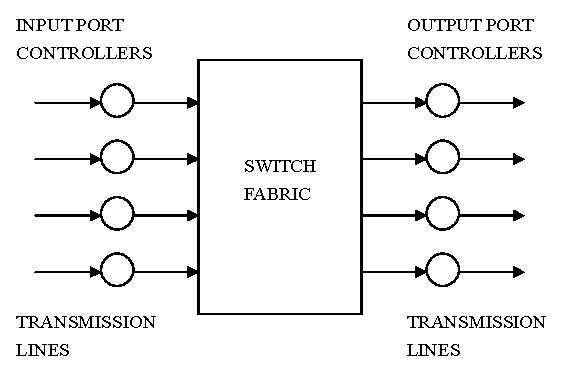
\includegraphics[width=.4\textwidth]{atmSwitch.eps}
\end{center}
\caption{An Overview of the Switch Fabric} \label{fig:atmSwitch}
\end{figure}


The switch fabric switches cells from input controllers to output
controllers. If different input controllers inject cells into the
fabric at the same time which are destined for the same output port
controller, then only one will initially succeed. The others will be
rejected and must retry later. The fabric arbitrates
between such cells.

\begin{figure}[tbph]
\begin{center}
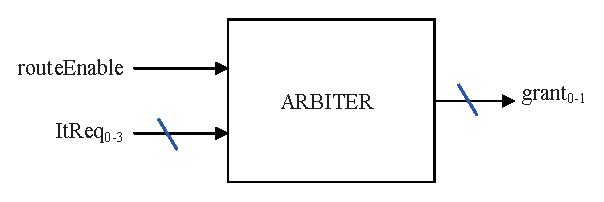
\includegraphics[width=.4\textwidth]{Arbiter.eps}
\end{center}
\caption{An Overview of the Arbiter} \label{fig:arbiter}
\end{figure}

In fact, there are $N$ arbiters in a $N \times N$ fabric switch,
each of which is in charge of the arbitration for requests from all
input ports which are destined for an output port. Because the
structure of an arbiter is the same as that of any other one,  we
only analyze one arbiter. An overview of the structure of an
arbiter design is shown in Fig. \ref{fig:arbiter}.

The arbiter enforces an arbitration policy for a single output port.
It takes inputs as a request vector, $ItReq$, indicating which inputs
are making requests for the output. %There are also two inputs
 %routeEnable$ and $frameStart$ which indicates when an arbitration
%within a frame should be made.

Its output is a grant vector which indicates the encoding of the
input whose request is currently valid. %Another output $outDisable$
%indicates whether the $grant$ node is currently valid.
For instance,
$ltReq[0:3]=[\mathsf{tt},\mathsf{ff},\mathsf{tt},\mathsf{ff}]$, and after
one cycle of arbitration, the output changes to the following
status: %$outDisable=\mathsf{ff}$, and
$grant[0:1]=[\mathsf{ff},\mathsf{ff}]$. This means that the first and
third input ports  make requests, and the first input port is
granted to transfer the data.

Round-robin is an important arbitration policy which is extensively
adopted in network systems. In general, the request, which has the
highest priority in round-robin order, will be granted in each
cycle.  We will explain formally the round-robin policy in the following
sections. This policy guarantees fairness (no starvation) among
requests and allows a request granted whose round-robin turn is
later and who is ready now. The ready request will be granted at
last if this request is kept ready.  The worst-case waiting time of
this
request can also be predicted. %  if this request is set and kept
%high.
This reliable prediction is another advantage of the round-robin policy. %, which depends on the last request granted and current ready requests. %There is an upper-bound for the ready request to be
%granted if this request is kept.
 Obviously, this is a response property. %
%worst-case wait time is proportional to the number of
%requestors minus one.
The round-robin arbiter works as follows. In
each cycle, one of the requests (in round-robin order) has the
highest priority to be granted. If the token-holding master does not
need the resource in this cycle, the master with the next highest
priority who sends a request can be granted the resource, and the
highest priority master then passes the token to the next master in
round-robin order.

 \subsection{STE and GSTE}
 STE  is a formal verification technique that is based on ternary
 symbolic simulation. In STE, specifications are given as  assertions
 of the form $ant\leadsto cons$ where both $ant$ and $cons$ are
 trajectory formulae. $ant$ is called the antecedent, which specifies
 with symbolic values that are used to drive the simulation. $cons$
 is called the consequent, which specifies the expected results of
 the
 simulation. %A Assertions specify a set of design properties in a
 %restricted temporal logic form.
 An STE tool such as FORTE can automatically check whether a given
 circuit $C$ satisfies a given STE assertion. If so, we write
 $\mathsf{cktSat}\ C\ ant\leadsto cons$.



 Four values $\mathsf{ff}$, $\mathsf{tt},$ $\mathsf{X}$, and
 $\mathsf{\top }$ are used in STE simulation
 \cite{CarFmBySymEvaOfPartTraj}. $\mathsf{ff}$ and
 $\mathsf{tt}$ have the same values as before. The third value
 $\mathsf{X}$ stands for an unknown value, while the fourth value
 $\top $ a
 clash value. Formally, we define $\mathbb{V}$$=_{df}\left\{ \mathsf{ff},%
 \mathsf{tt},\mathsf{X},\mathsf{\top }\right\} $.

 The first concept is the circuit model used for STE.  A circuit is
 modeled by a netlist, which is a set of nodes (or wires) connected
 by logical entities such as gates and one-phase delays. Gates
 describe combinational logics deciding the relationship between
 values of nodes. Delays refer to all sequential elements which can
 keep a "state". A  circuit state is an instantaneous snapshot of a
 circuit behavior  given by an  assignment of $\mathbb{V}$ to nodes
 of the circuit.

% %Here we use a type $\mathtt{node}$ to represent type of nodes. A
%% %circuit state is an instantaneous snapshot of a circuit behavior
%% %given by an
%% %assignment of lattice values to nodes of the circuit. Therefore, type $%
%% %\mathtt{state}\mathtt{=node}\ \Rightarrow \mathtt{boolPairs}$ is
%% %defined. A
%% %state sequence assigns a state to a time point. Here we still use $\mathsf{%
%% %nat}$ to define the type $\mathsf{time}$. Thus, we define $\mathtt{%
%% %stateSeq=time}\Rightarrow \mathtt{state}$.

% Here we adopt the proposal in \cite{DBLP:conf/csr/RoordaC06,Li09}
 %for the state transition function of a circuit. This state
%transition function defines not only the information propagation
%forwards from one time point to next time point, but also those
%occurring instantaneously through the combinational parts in a time
%point. For each circuit $c$, we can induce a next state functor
%operator $Y::\mathtt{stateSeq\Rightarrow stateSeq}$ such that $Y\ \
%$is a closure function. Roughly speaking, the words "a closure
%function $Y\ \ $" means that applying $Y\ \ $once can derive a
%closure of
%information in some form. %For instance, $\mathsf{fclosure%
%}\ nl\ s$ is a closure of information on the result simulation state
%of a circuit $nl$ at the driving state $s$.
%In detail, (1) $Y\ \ $ is \emph{monotonic}, $Y\ \ x\sqsubseteq Y\ \ y$ if $%
%x\sqsubseteq y%\footnote{%
%Here the relation $\leq $ is some kind of partial order. In lattice domain, $%
%\sqsubseteq $ is a partial order.} .$ (2) $Y\ \ $is
%\emph{idempotent}: $Y\ \ x=Y\ \ \left( Y\ \ x\right) $; (3) $Y\ \
%$is \emph{extensive}: $x\sqsubseteq Y\ \ x$. See \cite{Li09} for
%detailed account. %In STE, a circuit model $M:\mathtt{state\Rightarrow
%state}$ are represented by a next-state function from state to
%state. This $Y$ is also known as an excitation function, which is
%constructed on-the-fly during simulation, from the netlist
%description of the circuit.


 Here we use a simple example to illustrate the
 concepts used in STE verification. Fig. \ref{fig:memory} shows a
 netlist of 2-cell single-bit memory, which is modified from a GSTE
 tutorial \cite{DBLP:conf/atva/Yang06}.\\

 \begin{figure}[tbph]
 \begin{center}
 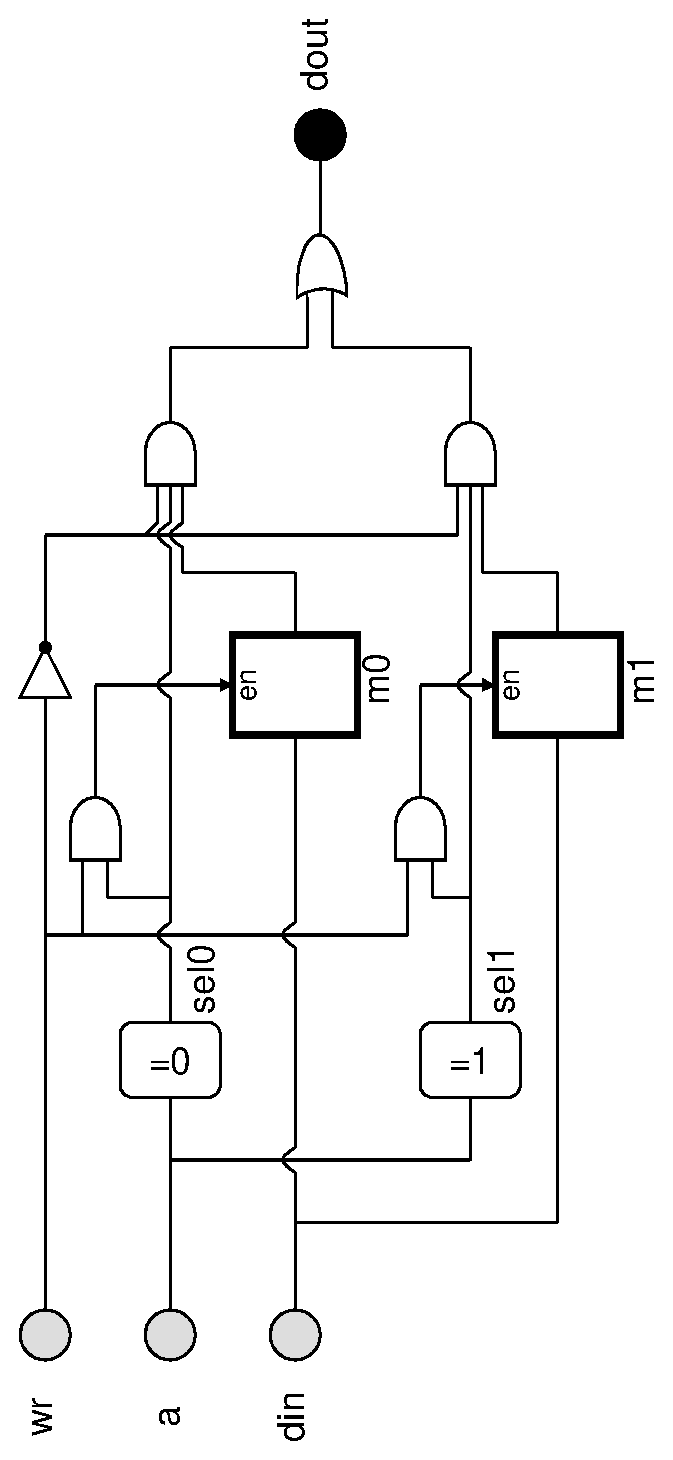
\includegraphics[angle=270, width=.4\textwidth]{memory.eps}
 \end{center}
 \caption{2-cell single-bit memory} \label{fig:memory}
 \end{figure}
%% %The excitation function $Y$ is as follows:

%% %$Y\ s\ m_{0}=((s\ wr\wedge  _{4}\lnot _{4}s\ a)\rightarrow _{4}s\ din)\wedge
%% %_{4}((\lnot _{4}s\ wr\vee _{4}s\ a)\rightarrow _{4}s\ m_{0})$

%% %$Y\ s\ m_{1}:((s\ wr\wedge  _{4}s\ a)\rightarrow _{4}s\ din)\wedge ((\lnot _{4}s\
%% %wr\vee _{4}\lnot _{4}s\ a)\rightarrow _{4}s\ m_{1})$$write=\mathsf{AndList}[\mathsf{Is1}\ wr,din\ \mathsf{isB}\ bD,a\

 Let\  $write=\mathsf{AndList}[\mathsf{Is1}\ wr,din\ \mathsf{isB}\
 bD,a\ \mathsf{isB}\ bA]$, $retain=\mathsf{AndList}[wr\ \mathsf{isB}\
 bWr$, $When\ bWr\ (a\
 \mathsf{isB}\ \lnot bA)]$, $read=\mathsf{AndList}[\mathsf{%
 Is0}\ wr,a\ \mathsf{isB}\ bA],$ $outResult=dout\ \mathsf{isB}\ bD$.
 Here $\mathsf{Is1}$($\mathsf{Is0}$)\ $wr$ simply specifies that the
 value of the node $wr$ is $\mathsf{tt}$($\mathsf{ff}$), and
 $\mathsf{AndList}\ fs$ is a conjunction of trajectory formulae list
 $fs$. $\mathsf{When}\ b \ f$ specifies that only when the Boolean
 expression $b$ is true, the trajectory formula $f$ holds, otherwise
 all the nodes are set the value $\mathsf{X}$.
 The notation $din\ \mathsf{isB}\ bD$ simply abbreviates $ \mathsf{%
 AndList\ [When\ }bD\ (\mathsf{Is1}\ din),\mathsf{When\ \lnot }bD\ (\mathsf{Is0}%
 \ din)]$, which assigns a symbolic value $bD$ to the node $din$. A
 novel trajectory formula \textsf{chaos} is introduced here to
 represent a state where the values of all the nodes in the circuit
 are unknown. We also define $\mathsf{Next^1}\ f=\mathsf{Next}\ f$,
 $\mathsf{Next^{N+1}}\ f=\mathsf{Next}\ (\mathsf{Next}^{N}\ f)$.
For notation convenience, we also introduce a syntactical
abbreviation for symbolic value assignments to vectors :
$ns\mathsf{\ bvAre\ }bvs\equiv \mathsf{AndList}\ (\mathsf{map}\
\mathsf{isB}\ (\mathsf{zip}\ ns\ bvs))$.

 Let\  $ant$=$\mathsf{AndList}[write, \mathsf{Next}\ retain,
 \mathsf{Next^2}\ read]$, $cons=\mathsf{Next^2}\ outResult$. The STE
 assertion $ant\leadsto cons$ specifies that if a value is written to
 a memory cell, and no other writes to the cell in the next cycle,
 then the read from the cell immediately  later will return the value.

 One of the main  limitations of STE is that it can only deal with
 properties ranging over a finite number of time steps. Generalized
 Symbolic Trajectory Evaluation (GSTE) is an extension of STE that
 can deal with properties ranging over unbounded time
 \cite{YangS03,yangTech,DBLP:conf/iccad/YangG02}.
 In GSTE, specifications on circuits are given by assertion graphs, which are $%
 \forall$-automata. Fig. \ref{fig:memoryGsteGraph} shows an
 assertion graph for the netlist in Fig. \ref{fig:memory}. This
 assertion graph  specifies that if a value is written to a memory
 cell, and no other writes to the cell in the next cycle, then the
 read from the cell immediately will return the value.

 \begin{figure}[tbph]
 \begin{center}
 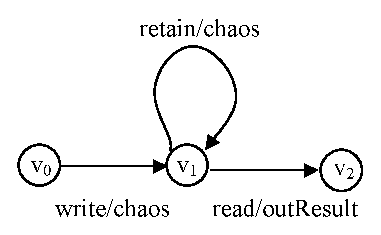
\includegraphics[width=.4\textwidth]{memoryGraph.eps}
 \end{center}
 \caption{GSTE assertion graph for memory cell}
 \label{fig:memoryGsteGraph}
 \end{figure}


 An STE assertion such as the aforementioned one $ant\ \leadsto\
 cons$ can be seen as a linear assertion graph shown as (b) in Fig.
 \ref{fig:gsteGrapgCollections}. While a  GSTE assertion
 graph with loops such as Figure \ref{fig:memoryGsteGraph} can
 be seen as a collection of linear assertion graphs.

 \begin{figure}[tbph]
 \begin{center}
 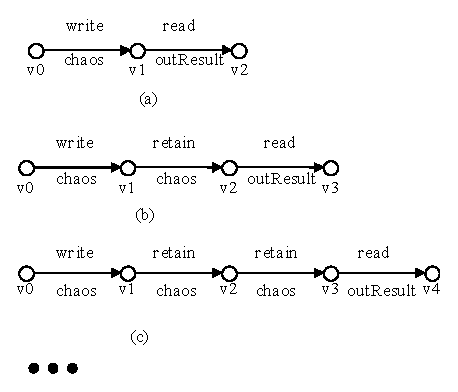
\includegraphics[width=.4\textwidth]{gsteCollections.eps}
 \end{center}
 \caption{STE assertions and GSTE assertion graphs}
 \label{fig:gsteGrapgCollections}
 \end{figure}
%% %Suppose that $sq$ is state sequence such that $sq\ 0$
%% %$a=\mathsf{tt},$ $sq\ 0\ wr=\mathsf{tt},$ $sq\ 0\ din=\mathsf{tt},$
%% %and $sq\ 0\ n=\mathsf{X}$ for any other nodes $n$, and $sq\ 1$
%% %$wr=\mathsf{ff},$ $sq\ 1\ n=\mathsf{X}$ for any other nodes $n$,
%% %$mem$ is the next state function for the circuit in Figure
%% %\ref{fig:memory}, after one simulation step for the circuit is
%% %finished, then the result state sequence $mem$ $sq$ after simulation
%% %satisfies that $mem$ $sq\ 0\ n=sq\ 0\ n$ if $n\in
%% %\{wr,a,din,m_{0},m_{1},out\}, $ $mem$ $sq\ 0\ sel_{0}=\mathsf{ff},$ $mem$ $%
%% %sq\ 0\ sel_{1}=\mathsf{tt}.$ At the second point, $mem$ $sq\ 1\ m_{1}=%
%% %\mathsf{tt,}$ $mem $ $sq\ 1\ n=sq\ 1\ n$ for any other nodes $n.$


\subsection{HOL specification of One Round-Robin Arbitration}

This subsection is mainly taken from HOL specification of
round-robin arbitration in the counterpart section in \cite{Paul94}.
Given an indication of the last value selected, round robin
arbitration returns the next highest value requested, with suitable
wrap around from the highest possible request to the lowest.

\vspace{2mm}
\begin{specification}
$\mathtt{let\ SUC\_MODN\ N\ last=}$\\

\>$\mathtt{(last+1=N)=>\ 0|\ (last+1);}$\\
\\

$\mathtt{letrec\ RoundRobin\ 0\ requestSet\ last\ N=0}$\\

$\mathtt{/\backslash \ RoundRobin\ n\ requestSet\ last\ N=}$\\

\>$\mathtt{let\ tryNext=SUC\_MOD\ N\ last\ in}$\\

\>$\mathtt{((tryNext\ mem\ requestSet)=>\ tryNext}$\\

\>$\mathtt{|RoundRobin\ (n-1)\ requestSet\ tryNext \ N);}$\\

\\

$\mathtt{let\ RoundRobinArbiter\ N\ requestSet\ last=}$\\

\>$\mathtt{(requestSet=[])=>NORESULT|}$\\

\>$(\mathtt{RESULT\ (RoundRobin\ N\ requestSet\ last\ N));}$\\
\end{specification}

  The round-robin arbitration is specified by the function $\mathsf{%
RoundRobinArbiter}$ which has several arguments: the number of input ports, $%
N$; a list giving the input ports making requests, $requestSet$; and
the last successful input port in the previous arbitration. It
returns either an
indication that it cannot make a selection if the request set is empty ($%
\mathsf{NORESULT}$); otherwise it returns the result of the round robin
arbitration. A result is of a datatype defined as follows:

$\mathtt{ROUNDTTYPE= NORESULT\ |\ RESULT\ int}$

The function $\mathsf{RoundRobin}$ is called in $\mathsf{RoundRobinArbiter}$%
. It tries successively higher values above the last successful
request until it finds a proper request in the request set. It is
defined in terms of a counter ensures   that the function does
terminate. Provided that the counter is initially set the value of
the highest request possible and the request set is not empty, it
will not terminate until a result is obtained.

For instance, for an arbitrator of the $4\times 4$   switch fabric,
the last successful input port number in the previous arbitration is
0, and the current request set is [0,2,3], we call
$\mathsf{RoundRobinArbiter}\ 4\ [0,2,3]\ 0$=$2$, which returns 2 as
the result in the current round of arbitration.

The function $\mathsf{RoundRobinArbiter}$ gives a good explanation
on round-robin arbitration in mathematical notation in the sense
that a request and a grant result are represented by an integer and
request set an integer set. However, this notation is far away from
the structure of the arbiter shown in Fig. \ref{fig:arbiter}. For
instance, request sets are represented by a vector of inputs $req_0
--req_3$ and the number of the  granted input port is encoded in a
vector in Fig. \ref{fig:arbiter}. We need to give another specification
which considers more details of hardware implementation of the
arbiter.

 \vspace{2mm}
 {\footnotesize
\begin{specification}
$\mathtt{let\ RequestsToArbitrate\ 0\ reqVect=[]}$\\

$\mathtt{/\backslash RequestsToArbitrate\ n\ reqVect=}$\\

\>$\mathtt{ (reqVect\ !\ (n-1))=>}$\\

\>$\mathtt{([n-1]\ union\ (RequestsToArbitrate\ (n-}1)\
reqVect)$\\

\>$\mathtt{  |RequestsToArbitrate\ (n-1)\ reqVect}$
\end{specification}}

The argument of $requestSet$ in the function
$\mathsf{RoundRobinArbiter}$ is a list of integer numbers. However,
the request set is represented by the Boolean values of a request
vector in the hardware implementation of the arbiter. Let\ $reqVect$
be a Boolean vector with each bit indicating whether a corresponding
input is making a request, $\mathsf{RequestsToArbitrate}$ returns
the set of requests by scanning each bit in turn. If it holds the
value $\mathsf{tt}$, then its position number is added to the
request set. For instance, let\
$reqVect[0:3]=[\mathsf{tt},\mathsf{ff},\mathsf{tt},\mathsf{tt}]$, then
$\mathsf{RequestsToArbitrate}\ 4\ reqVect=[0,2,3]$. \vspace{2mm}
{\footnotesize
\begin{specification}
$\mathtt{let\ SucessFulInput\ last\ reqVect=}$\\

$\mathtt{\ \ (let\ requestSet=}$\\
$\mathtt{\ \ RequestsToArbitrate\ (len\ req)\ reqVect\ in}$%
\\

$\mathtt{\ \ RoundRobinArbiter\ (len\ req)\ requestSet\ last}$\\

\\

$\mathtt{let\ GrantForOut\ reqVect\ grantVect=}$\\

$\mathtt{\ \ let\ sucIn=SucessFulInput\ (decode\ grantVect)\ reqVect\ in}$\\

$\mathtt{\ \ (sucIn=NORESULT)=>grantVect}$\\

$\mathtt{\ \ \ |(val\ (RESULT\ result=sucIn)\ in}$\\

$\mathtt{\ \ \ \ \ encode\ (len\ grantVect)\ result}))$
\end{specification}}
\vspace{2mm}

 Giving a $grantVect$ indicating the value of the last
successful input port in the previous arbitration, and $reqVect$ be
a Boolean vector with each bit
indicating whether a corresponding input is making a request, $\mathsf{%
GrantForOut}\ reqVect \ grantVect$ first converts $grantVect$ to an
integer, then calls $SucessFulInput$ to compute the   successful
input, and converts the integer result to another Boolean vector,
which encodes the
result of this arbitration. For instance, let\  $reqVect[0:3]=[\mathsf{tt},\mathsf{ff},\mathsf{tt},\mathsf{tt}]$,
$grantVect[0:1]=[\mathsf{ff},\mathsf{ff}]$, then $%
\mathsf{GrantForOut}\ reqVect \
grantVect[0:1]=[\mathsf{ff},\mathsf{tt}]$ which denotes that $reqVect[2]$ is granted.




\section{STE Specification of One Round of the Round-Robin Arbitration}
\label{sec:STESpecRoundRobin}
 According to the above discussion, we
can show the truth table of the round-robin arbitration function in
Table \ref{truthTable},
which is corresponding to one round of round-robin arbitration $\mathsf{%
GrantForOut}\ req \ grant$. Here $req$ stands for a vector
$req_0--req_3$, and $grant$ a vector of $grant_0,grant_1$. The
returned result is another vector $grant'_0, grant'_1$. This is also
the base of the implementation of the logics
 of the arbitration.
Among the %This function takes
six arguments, $%
req_0--req_3$ stand for four request inputs, and $grant_0, grant_1$ for the
encoding of the granted request in the previous arbitration round. $%
grant'_0, grant'_1$ are the outputs to indicate the
encoding vector of the number of the granted ports. Here we omit the
other inputs $frameStart$, $routeEnable$ and $reset$  of the
arbiter, which is not the main factors affecting the state space.
This table is a typical use of the special value $\mathsf{X}$, which
significantly reduces the size of the truth-table and the synthesis
size of the logic of the arbiter.


\begin{center}
\begin{table}[tbp]
\caption{Ternary-valued Truth Table of the Round-robin Arbiter}
\label{truthTable}
\begin{center}
\begin{tabular}{llllllll}
req0 & req1 & req2 & req3 & $grant_0$ & $grant_1$ & $grant'_0$ & $grant'_1$ \\
$\mathsf{X}$ & $\mathsf{ff}$ & $\mathsf{ff}$ & $\mathsf{ff}$ &
$\mathsf{ff}$
& $\mathsf{ff}$ & $\mathsf{ff}$ & $\mathsf{ff}$ \\
$\mathsf{X}$ & $\mathsf{tt}$ & $\mathsf{X}$ & $\mathsf{X}$ &
$\mathsf{ff}$ &
$\mathsf{ff}$ & $\mathsf{tt}$ & $\mathsf{ff}$ \\
$\mathsf{X}$ & $\mathsf{ff}$ & $\mathsf{tt}$ & $\mathsf{X}$ &
$\mathsf{ff}$
& $\mathsf{ff}$ & $\mathsf{ff}$ & $\mathsf{tt}$ \\
$\mathsf{X}$ & $\mathsf{ff}$ & $\mathsf{ff}$ & $\mathsf{tt}$ &
$\mathsf{ff}$
& $\mathsf{ff}$ & $\mathsf{tt}$ & $\mathsf{tt}$ \\
$\mathsf{ff}$ & $\mathsf{X}$ & $\mathsf{ff}$ & $\mathsf{ff}$ &
$\mathsf{tt}$
& $\mathsf{ff}$ & $\mathsf{tt}$ & $\mathsf{ff}$ \\
$\mathsf{X}$ & $\mathsf{X}$ & $\mathsf{tt}$ & $\mathsf{X}$ &
$\mathsf{tt}$ &
$\mathsf{ff}$ & $\mathsf{ff}$ & $\mathsf{tt}$ \\
$\mathsf{X}$ & $\mathsf{X}$ & $\mathsf{ff}$ & $\mathsf{tt}$ &
$\mathsf{tt}$
& $\mathsf{ff}$ & $\mathsf{tt}$ & $\mathsf{tt}$ \\
$\mathsf{tt}$ & $\mathsf{X}$ & $\mathsf{ff}$ & $\mathsf{ff}$ &
$\mathsf{tt}$
& $\mathsf{ff}$ & $\mathsf{ff}$ & $\mathsf{ff}$ \\
$\mathsf{ff}$ & $\mathsf{ff}$ & $\mathsf{X}$ & $\mathsf{ff}$ &
$\mathsf{ff}$
& $\mathsf{tt}$ & $\mathsf{ff}$ & $\mathsf{tt}$ \\
$\mathsf{X}$ & $\mathsf{X}$ & $\mathsf{X}$ & $\mathsf{tt}$ &
$\mathsf{ff}$ &
$\mathsf{tt}$ & $\mathsf{tt}$ & $\mathsf{tt}$ \\
$\mathsf{tt}$ & $\mathsf{X}$ & $\mathsf{X}$ & $\mathsf{ff}$ &
$\mathsf{ff}$
& $\mathsf{tt}$ & $\mathsf{ff}$ & $\mathsf{ff}$ \\
$\mathsf{ff}$ & $\mathsf{tt}$ & $\mathsf{X}$ & $\mathsf{ff}$ &
$\mathsf{ff}$
& $\mathsf{tt}$ & $\mathsf{tt}$ & $\mathsf{ff}$ \\
$\mathsf{ff}$ & $\mathsf{ff}$ & $\mathsf{ff}$ & $\mathsf{X}$ &
$\mathsf{tt}$
& $\mathsf{tt}$ & $\mathsf{tt}$ & $\mathsf{tt}$ \\
$\mathsf{tt}$ & $\mathsf{X}$ & $\mathsf{X}$ & $\mathsf{X}$ &
$\mathsf{tt}$ &
$\mathsf{tt}$ & $\mathsf{ff}$ & $\mathsf{ff}$ \\
$\mathsf{ff}$ & $\mathsf{tt}$ & $\mathsf{X}$ & $\mathsf{X}$ &
$\mathsf{tt}$
& $\mathsf{tt}$ & $\mathsf{tt}$ & $\mathsf{ff}$ \\
$\mathsf{ff}$ & $\mathsf{ff}$ & $\mathsf{tt}$ & $\mathsf{X}$ &
$\mathsf{tt}$
& $\mathsf{tt}$ & $\mathsf{ff}$ & $\mathsf{tt}$%
\end{tabular}%
\end{center}
\end{table}
\end{center}

Note that this truth-table is exhaustive, which explores all the cases of
the input patterns. Here we briefly analyze why the truth-table is
exhaustive. Note that we have to analyze all the possible boolean
assignments for the nodes $grant_0, grant_1$, namely, $\mathsf{X}$ is not used
to assign the value of the two nodes. $X$ value is mainly used for value
assignments of the nodes $req_0--req_3$. For instance, when (a) $grant_0=%
\mathsf{ff}$ and $grant_1=\mathsf{ff}$, then we have either (0) $req_1=%
\mathsf{ff} \wedge req_2=\mathsf{ff} \wedge req_3=\mathsf{ff}$, or (1) $req_1=%
\mathsf{tt}$, or (2) $req_2=\mathsf{tt}$, or (3)$req_3=\mathsf{tt}$. The
four cases are corresponding to  lines from the first one to the fourth  one in the
table \ref{truthTable}, and also list all the possible cases when $grant_0=\mathsf{ff}$%
, and $grant_1=\mathsf{ff}$. In case (0), the input value of $req_0$
is not
cared by us because the arbitration value of $grant'_0$ and $%
grant'_1$ will be the same as $grant_0$ and $grant_1$
respectively in
both input cases $req_0=\mathsf{ff}$ and $req_0=\mathsf{tt}$. In case (1), $%
req_1$ is the highest priority request in the current round, and will be
granted immediately once $req_1=\mathsf{tt}$. Therefore, the values
assignments for the nodes $req_2$, and $req_3 $ are not cared by us. In case
(2), $req_2$ is the highest priority request in the current round if $req_1=%
\mathsf{ff}$, and will be granted immediately. Therefore, the values
assignments for the nodes $req_3 $ are not cared by us. In case (3), $req_3$
is the highest priority request in the current round if $req_1=\mathsf{ff}$
and $req_2=\mathsf{ff}$, and will be granted immediately.

Similarly, we can analyze the cases of the other boolean assignments
for the nodes $grant_0, grant_1$. In fact each of  these cases is
symmetric to
case (a) in some sense. For instance, the input assignments for nodes $%
req_0--req_3$ can also be divided into four subcases in the case where $%
grant_0=\mathsf{tt}$ and $grant_1=\mathsf{ff}$, each of which is
corresponding to the counterpart one in the case (a) by shifting the
input assignments for nodes $req_0--req_3$ by one bit in the right
direction in Table \ref{truthTable}. At last, we analyze the
complexity of the verification in the term of the number of
requests $N$. The number of all the Boolean simulation cases is $2^N\times N$%
, however that of the ternary valued simulation cases  is only $N
\times N$ with the help of the $\mathsf{X}$ value assignments.
Notice that this is a substantial decrease at the exponential scale.

According to  table \ref{truthTable}, we can easily write an STE
assertion, as shown in table \ref{tabConstrSTE}:
\begin{center}
\begin{table}
\caption{An STE assertion for one-round
arbitration}\label{tabConstrSTE}
\begin{specification}

$\mathtt{constr\_0\_0=   \neg grantV_0\wedge \neg grantV_1\wedge \neg
reqV_1\wedge \neg
reqV_2\wedge \neg reqV_3  }$\\

$\mathtt{constr\_0\_1=   \neg grantV_0\wedge \neg grantV_1\wedge reqV_1  }$\\

$\mathtt{constr\_0\_2= \neg grantV_0\wedge \neg grantV_1\wedge \neg reqV_1\wedge reqV_2 }$\\

$\mathtt{constr\_0\_3= \neg grantV_0\wedge \neg grantV_1\wedge \neg
reqV_1\wedge \neg reqV_2\wedge reqV_3 }$\\


$\mathtt{constr\_1\_1= grantV_0\wedge \neg grantV_1\wedge \neg
reqV_2\wedge \neg
reqV_3\wedge \neg reqV_0 }$\\

$\mathtt{ constr\_1\_2= grantV_0\wedge \neg grantV_1\wedge reqV_2  }$\\

$\mathtt{constr\_1\_3= grantV_0\wedge \neg grantV_1\wedge \neg reqV_2\wedge reqV_3}$\\

$\mathtt{constr\_1\_0= grantV_0\wedge \neg grantV_1\wedge \neg
reqV_2\wedge \neg
reqV_3\wedge reqV_0}$\\

$\mathtt{constr\_2\_2= \neg grantV_0\wedge grantV_1\wedge \neg
reqV_1\wedge \neg reqV_3\wedge \neg
reqV_0 }$\\

$\mathtt{constr\_2\_3= \neg grantV_0\wedge grantV_1\wedge reqV_3  }$\\

$\mathtt{constr\_2\_0= \neg grantV_0\wedge grantV_1\wedge \neg  reqV_3\wedge reqV_0 }$\\

$\mathtt{constr\_2\_1= \neg grantV_0\wedge grantV_1\wedge reqV_1\wedge
\neg reqV_3\wedge \neg
reqV_0 }$\\

$\mathtt{constr\_3\_3= grantV_0\wedge grantV_1\wedge \neg reqV_1\wedge
\neg reqV_2\wedge \neg
reqV_0 }$\\

$\mathtt{constr\_3\_0= grantV_0\wedge grantV_1\wedge reqV_0 }$\\

$\mathtt{constr\_3\_1= grantV_0\wedge grantV_1\wedge reqV_1\wedge \neg reqV_0 }$\\

$\mathtt{constr\_3\_2=grantV_0\wedge grantV_1\wedge \neg reqV_1\wedge reqV_2\wedge \neg reqV_0}$\\

%\end{specification}

%\begin{specification}

$\mathtt{cons_0= When\ constr\_0\_0\  \ (AndList [Is0\ grant_0,Is0\  grant_1])}$\\

$\mathtt{cons_1=When\ constr\_0\_1\ \ (AndList [Is1\
grant_0,Is0\  grant_1])}$\\

$\mathtt{cons_2=When\ constr\_0\_2\  \
(AndList [Is0\  grant_0,Is1\  grant_1])}$\\

$\mathtt{cons_3= When\ constr\_0\_3\  \ (AndList [Is1\  grant_0,Is1\  grant_1])}$\\


$\mathtt{cons_4=When\ constr\_1\_1\  \
(AndList [Is1\  grant_0,Is0\  grant_1])}$\\

$\mathtt{ cons_5= When\ constr\_1\_2\   \ ( AndList [Is0\
grant_0,Is1\  grant_1])}$\\

$\mathtt{cons_6=When\ constr\_1\_3\   \
(AndList   [Is1\  grant_0,Is1\  grant_1])}$\\

$\mathtt{cons_7=When\ constr\_1\_0\    \  (AndList [Is0\  grant_0,Is0\  grant_1])}$\\

$\mathtt{cons_8= When\ constr\_2\_2 \   \ ( AndList [Is0\  grant_0,Is1\  grant_1])}$\\

$\mathtt{cons_9= When\ constr\_2\_3\    \ (AndList [Is1\
grant_0,Is1\  grant_1])}$\\

$\mathtt{cons_{10}=When\ constr\_2\_0\   \ (
AndList [Is0\  grant_0,Is0\  grant_1])}$\\

$\mathtt{cons_{11}=When\ constr\_2\_1\   \  ( AndList [Is1\  grant_0,Is0\  grant_1])}$\\

$\mathtt{cons_{12}=When\ constr\_3\_3\   \ ( AndList [Is1\  grant_0,Is1\  grant_1])}$\\

$\mathtt{cons_{13}=When\ constr\_3\_0\   \ (AndList [Is0\
grant_0,Is0\
grant_1])}$\\

$\mathtt{cons_{14}=When\ constr\_3\_1\   \ ( AndList
[Is1\  grant_0,Is0\  grant_1])}$\\

$\mathtt{cons_{15}=When\ constr\_3\_2\
   \ (AndList [Is0\  grant_0,Is1\  grant_1])}$\\

$\mathtt{ant=AndList [grant\ bvAre\ grantV,req\ bvAre\ reqV]}$\\

$\mathtt{cons= AndList [ \ cons_0,  \ cons_1,..., \ cons_{15}]}$\\

$\mathtt{assert=ant \leadsto \ Next\ cons}$\\



\end{specification}
\end{table}
\end{center}


Here   $grant$ is the vector of nodes  $[grant_0,grant_1]$, $grantV$
the vector of symbolic values $[grantV_0,grantV_1]$, $req$ the vector
of nodes  $[req_0,...,req_3]$, $reqV$ the vector of symbolic values
$[reqV_0,...,reqV_3]$. In FORTE, a node is simply of type string.
The antecedent $ant$ simply assigns symbolic values to the
corresponding nodes. For instance, node $grant_0$ is assigned the
symbolic value $grantV_0$. The consequent is a conjunction of
trajectory formulae, each of which is a guarded formula of the form
$\mathsf{When} \ constr_i \ cons_i$ and corresponding to each line
of the truth table listed in Table \ref{truthTable}. The assertion
$assert$ is an STE assertion which should be satisfied by one run
arbitration of the $4 \times 4$ round-robin
 arbiter. For such an STE assertion, we can directly run the tool
 FORTE to verify it.



\section{GSTE Specification of the sequential behaviors of the arbiter}
\label{sec:GSTE}
 In Table \ref{truthTable}, we only list the arbiter's
behavior in one round. In fact, its behavior is a typically
sequential, or reactive. It will accept the requests and make
arbitration in each cycle.  The sequential behavior can be precisely
captured by the following GSTE assertion graph in
Fig.\ref{fig:arbiterGraph}.
\begin{center}
\begin{table}
\caption{Antecedents of the GSTE specification in Fig.
\ref{fig:arbiterGraph}}
\begin{specification}
%$\mathtt{let\ rst = Is1 \  reset  ;}$\\

%$\mathtt{let\ nRst = Is0 \  reset ;}$\\

%$\mathtt{ let\ rtE=Is1 \  routeEnable ;}$\\

$\mathtt{let\ trans\_0\_1 = AndList [Is1 \
req1 ];}$\\

$\mathtt{let\ trans\_0\_2 = AndList [Is0 \ req1 , Is1 \
req2 ];}$\\

$\mathtt{let\ trans\_0\_3 = AndList [Is0 \ req1 , Is0 \ req2 , Is1 \
req3 ];}$\\

$\mathtt{let\ trans\_0\_0 = AndList [Is0 \ req1 , Is0 \ req2 , Is0 \
req3 ];}$\\

$\mathtt{let\ trans\_1\_2 = AndList [Is1 \ req2 ];}$\\

$\mathtt{let\ trans\_1\_3 = AndList [Is0 \ req2 , Is1 \
req3 ];}$\\

$\mathtt{let\ trans\_1\_0 = AndList [Is0 \ req2 , Is0 \ req3 , Is1 \
req0 ];}$\\

$\mathtt{let\ trans\_1\_1 = AndList [Is0 \ req2 , Is0 \ req3 , Is0 \
req0 ];}$\\

$\mathtt{let\ trans\_2\_3 = AndList [Is1 \ req3 ];}$\\

$\mathtt{let\ trans\_2\_0 = AndList [Is0 \ req3 , Is1 \
req0 ];}$\\

$\mathtt{let\ trans\_2\_1 = AndList [Is0 \ req3 , Is0 \ req0 , Is1 \
req1  ];}$\\

$\mathtt{let\ trans\_2\_2 = AndList [Is0 \ req3 , Is0 \ req0 , Is0 \
req1  ];}$\\

$\mathtt{let\ trans\_3\_0 = AndList [Is1 \
req0  ];}$\\

$\mathtt{let\ trans\_3\_1 = AndList [Is0 \ req0 , Is1 \
req1  ];}$\\

$\mathtt{let\ trans\_3\_2 = AndList [Is0 \ req0 , Is0 \ req1 , Is1 \
req2  ];}$\\

$\mathtt{let\ trans\_3\_3 = AndList [Is0 \ req0 , Is0 \ req1 , Is0 \
req2  ];}$\\
 \end{specification}
 \end{table}
 \end{center}

\begin{figure}[tbph]
\begin{center}
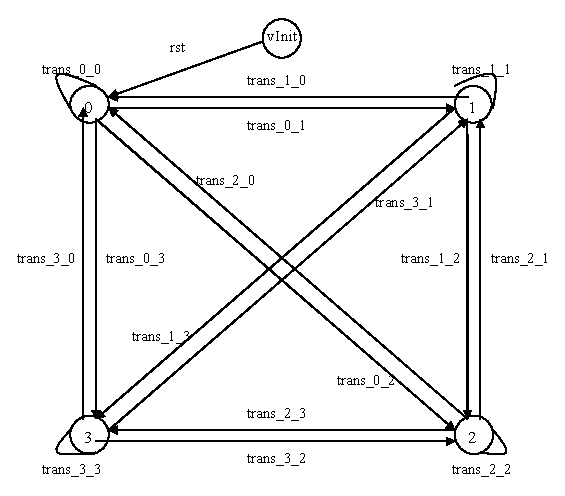
\includegraphics[width=.5\textwidth]{ArbiterGraph.eps}
\end{center}
\caption{GSTE specification of the Arbiter} \label{fig:arbiterGraph}
\end{figure}

The edge from $init$ to $v_0$ stands for the reset action which sets
the initial value of the register $grant_0, grant_1$ $\mathsf{ff}$
respectively. The node $v_0$ is corresponding to the   state where
$grant_0=\mathsf{ff}, grant_1=\mathsf{ff}$, the edge $(v_0, v_1)$
stands for the transition from state $v_0$ to $v_1$ where
$grant_0=\mathsf{tt}, grant_1=\mathsf{ff}$. The antecedent of the
transition is $trans\_0\_1$ which sets  $req1$ $\mathsf{tt}$,    and
doesn't care the values of any other inputs. At state $v_0$, once
the inputs $req1--req3$ are set $\mathsf{ff}$, the state
$grant_0=\mathsf{ff}, grant_1=\mathsf{ff}$ will hold. This is captured
by the self-loop $(v_0,v_0)$ whose antecedent is $trans\_0\_0$. Here
we omit the consequents below each edge in the graph because they
only specify the  values of nodes $grant_0,grant_1$ respectively.
These values are implicitly indicated by the   state nodes which the
edges come from.

Similarly, we can analyze the other states and transitions.


\section{GSTE Specification of the response property of the
arbiter}\label{secLiveness}



 For the $4\time 4$ round-robin arbiter, a running state of arbiter is
 determined  by the state variable vector $grant$. Therefore we
 sometimes call
 a state by   the decoding number of value of the $grant$ vector %$\mathsf{decode } \
 %grant$
at the state in the following part of this subsection. For instance,
If  we call a state 2, we mean that the decoding number of the value
of the $grant$ vector of the arbiter is 2.



 In this part, we will introduce how to model the
response property of the arbiter. This property specifies that  once a request $req_i$ is
set high from a state $i$ and kept high, then the request will be
granted after several cycles. The worst-case waiting time for the
request to be granted can also be predicted. Before we
 formally define the response property by GSTE assertion graphs, we give two examples to illustrate the response
 property.

 \begin{example}\label{livenessExample1}
Consider a state where the value of $grant$ is $[\mathsf{tt,ff}]$,
which means that the last request granted is $req_{1}$, if the
request $req_{3}$ is set high and kept high, then the request will
be granted (or the value of $grant$ is set $[\mathsf{tt,tt}]$) after
at most $2$ cycles. Namely, the  worst-case waiting time for
 this request to be granted is $2$.
\end{example}

\begin{example}\label{livenessExample2}
Consider a state where the value of $grant$ is $[\mathsf{ff,tt}]$,
which means that the last request granted is $req_{2}$, if the
request $req_{2}$ is set high again and kept high, then the request will
be granted (or the value of $grant $ is set $[\mathsf{ff,tt}]$
again) after at most $4$ cycles. Namely, the  worst-case waiting
time for
 this request to be granted is $4$.
\end{example}

\vspace{2mm}
\begin{center}
\begin{table}
\caption{Antecedents and Consequents of   GSTE specification in Fig.
\ref{figLiveness1}}
\begin{specification}
$\mathtt{let\ rst = Is1 \  reset  ;}$\\

%$\mathtt{let\ nRst = Is0 \  reset ;}$\\

%$\mathtt{ let\ rtE=Is1 \  routeEnable ;}$\\

%$\mathtt{let\ others=[nRst, rtE,Is1\ req3];}$\\
$\mathtt{let\ antSet= AndList\ [\mathsf{Is0}\ req0, \mathsf{Is1}\
req1,\mathsf{Is0}\ req2,\mathsf{Is0}\ req3]}$ \\

$\mathtt{let\ ants\_vSet\_2 = AndList [Is1\ req3,Is1\ req2];}$\\

 $\mathtt{let\  ants\_vSet\_3 = AndList [Is1\ req3,Is0\ req2 ];}$\\
$\mathtt{let\ ants\_2\_3 = AndList [Is1\ req3 ];
}$\\

%$ \mathtt{let\ cons\_2= AndList[Is1\ xGrant, Is0\ yGrant]; }$\\
 $\mathtt{let\ cons\_3=AndList[Is1 \ grant_0, Is1\ grant_1];}$\\
 \end{specification}

\end{table}
\end{center}


\begin{figure}[tbph]
\begin{center}
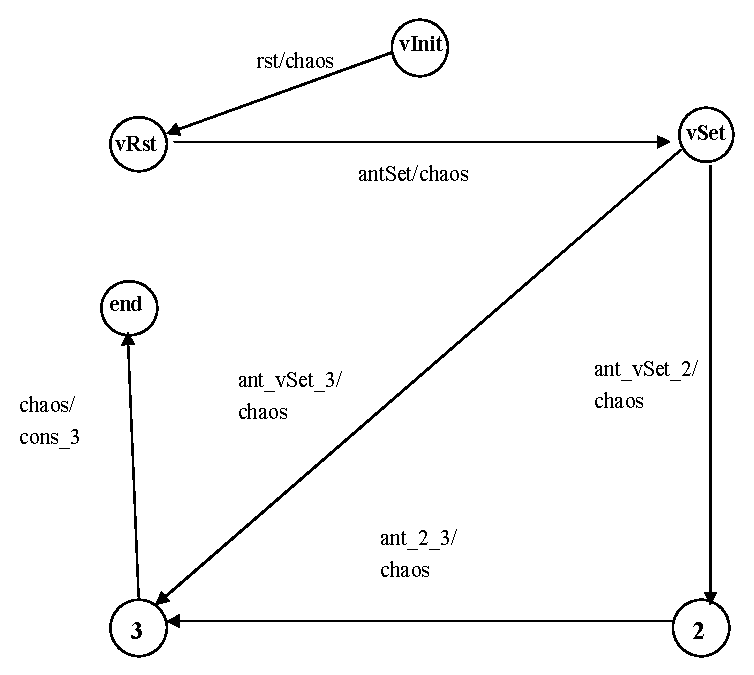
\includegraphics[width=.4\textwidth]{figLiveness1.eps}
\end{center}
\caption{STE specification of the response property in Example
\ref{livenessExample1}} \label{figLiveness1}
\end{figure}

%\begin{figure}[tbph]
%\begin{center}
%\includegraphics[width=.5\textwidth]{figLiveness2Spec.eps}
%\end{center}
%\caption{GSTE specification of the Arbiter} \label{fig:arbiterGraph}
%\end{figure}
\vspace{2mm}
\begin{center}

\begin{table}
\caption{Antecedents and Consequents of   GSTE specification in Fig.
\ref{figLiveness2}}


\begin{specification}
$\mathtt{let\ rst = Is1\ reset;}$\\
%$\mathtt{let\  nRst = Is0\ reset;}$\\
%$\mathtt{ let\  rtE = Is1\ routeEnable;}$\\
%$\mathtt{ let\ others=[nRst,rtE,Is1\ req2];}$\\
$\mathtt{let\ antSet= AndList\ [\mathsf{Is0}\ req0, \mathsf{Is0}\
req1,\mathsf{Is1}\ req2,\mathsf{Is0}\ req3]}$ \\
%$\mathtt{let\ consSet= AndList\ [\mathsf{Is0}\ xGrant, \mathsf{Is1}\
% yGrant]}$ \\
$\mathtt{ let\ ants\_vSet\_3 = AndList [ Is1\ req2,Is1\
req3]; }$\\
$\mathtt{let\ ants\_vSet\_0= AndList [Is1\ req2,Is0\ req3, Is1\ req0];}$\\
$ \mathtt{let\ ants\_vSet\_1 = AndList[Is1\ req2, Is0\ req3,Is0\ req0,}$\\
$ \ \ \ \ \ \ \ \ \ \ \  \ \ \ \ \  \mathtt{Is1\  req1]};$\\
 $\mathtt{let\ ants\_vSet\_2 = AndList [Is1\ req2,Is0\ req3, Is0\ req0,}$\\
 $ \ \ \ \ \ \ \ \ \ \ \ \ \ \ \ \ \ \mathtt{ Is0\ req1 ]};$\\
$ \mathtt{let\ ants\_3\_0=AndList [Is1\ req2,Is1\ req0]};$\\
$ \mathtt{let\ ants\_3\_1=AndList [Is1\ req2,Is0\ req0, Is1\ req1];}$ \\
$\mathtt{let\ ants\_3\_2=AndList [Is1\ req2,Is0\ req0, Is0\ req1,
 ];}$ \\
$ \mathtt{let\ ants\_0\_1= AndList [Is1\ req2,Is1\ req1];} $\\
 $\mathtt{let\ ants\_0\_2= AndList [Is1\ req2,Is0\ req1 ]};$\\

$ \mathtt{let\ ants\_1\_2= AndList [Is1\ req2 ]};$\\
 %$\mathtt{let\ cons\_0=AndList[Is0\ xGrant, Is0\ yGrant]};$\\
 %$\mathtt{let\ cons\_ 1=AndList [Is0\ xGrant, Is1\ yGrant];}$ \\
 $\mathtt{let\ cons\_ 2=AndList [Is0\ grant_0, Is1\ grant_1];}$ \\
 % $\mathtt{let\ cons\_ 3=AndList[Is1\ xGrant,Is1\ yGrant];}$
\end{specification}

\end{table}
\end{center}
\begin{figure}[tbph]
\begin{center}
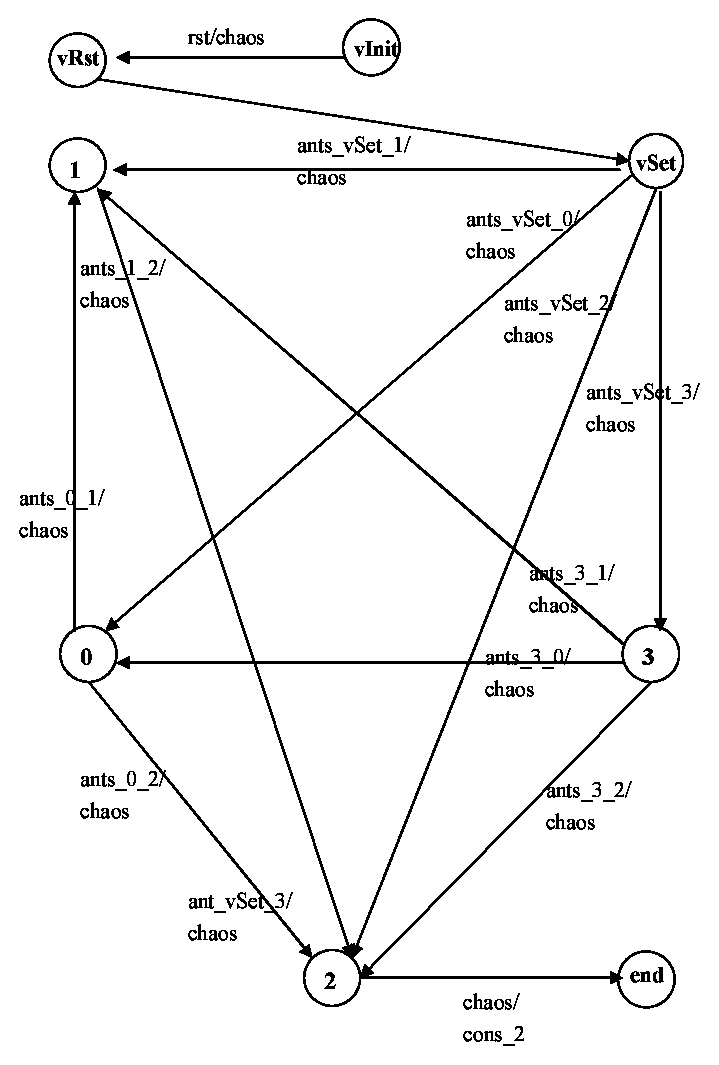
\includegraphics[width=.4\textwidth]{figLiveness2.eps}
\end{center}
\caption{GSTE specification of the response property in Example
\ref{livenessExample2}} \label{figLiveness2}
\end{figure}




We can formally model the two response properties in two GSTE graphs, which are shown in Fig.
\ref{figLiveness1} and Fig. \ref{figLiveness2}. Let\  us explain  the
reason why the two assertion graphs can naturally specify the
response properties.

In each of the GSTE assertion graphs, there is a state where the decoding value of $grant$
 vector is set as  some integer $s$ and the request $req_j$ is set high and kept
high until this request
 $req_j$ is granted. There are four  distinguishing features in the graphs:

\begin{description}
\item[(1)] The first edge $(\mathid{vInit}, \mathid{vRst})$
represents an action of reset, and the second edge
$(\mathid{vRst},\mathid{vSet})$ sets the state of the arbiter to
some initial value. For Fig. \ref{figLiveness1}, in order to set the
initial value of state variable vector $grant$
$[\mathsf{tt},\mathsf{ff}]$, we simply set the simulation constraint
by setting the antecedent of edge $(\mathid{vRst},\mathid{vSet})$ as
$\mathsf{AndList}\ [\mathsf{Is0}\ req_0, \mathsf{Is1}\
req_1,\mathsf{Is0}\ req_2,\mathsf{Is0}\ req_3]$, which means that
only request $req_1$ is set high and the others are set low. Thus
the
request  $req_1$ will be granted immediately, and the grant vector will be set $%
[\mathsf{tt,ff}] $ accordingly.

\item[(2)]There is a  node list $seq $ which
represents the state
 which may be reached from node $vSet$ by granting requests in a descending
priority order. Let $seq'=([vSet]@seq)$,
for any two indices $k,h$ such that $0\leq k<h< \mathsf{len}\ seq'$, there is an edge $(%
seq'_k,seq'_h)$ whose antecedent must include a formula
$\mathsf{Is1}\ req_j$, which means that the request $req_j$ is kept
high in the
simulation steps. The edge $(%
seq'_k,seq'_h)$ represents a simulation step where a request
$req_{seq'_h}$ is granted from state node $seq'_k$. In Fig.
\ref{figLiveness1} and Fig. \ref{figLiveness2}, $seq$ is $[2,3]$ and
$[3,0,1,2]$ respectively. In Fig. \ref{figLiveness1}, the edge
$(vSet,3)$ represents a simulation step whose constraint is
$\mathsf{AndList}\ [\mathsf{Is0}\ req_2,\mathsf{Is1}\ req_3]$, while
$(2,3)$   a simulation step whose constraint is $\mathsf{AndList}\
[\mathsf{Is1}\ req_3]$.




\item[(3)] %There is a terminal node $end$ which is
The last element of the list $seq'$ represents a state after $req_j$
is granted. It is connected with any other node $v$ in $seq'$ by an
edge. From this state node, we can test the value of $grant$ by an
edge which is from it to $end$ whose   consequent assigns the
decoding number of $j$ to $grant$. This means that the request
$req_j$ is granted at last.
 In Fig. \ref{figLiveness1} and
Fig. \ref{figLiveness2}, the last nodes of $seq'$ are labeled by 3 and 2
respectively.

\item[(4)]
The edges starting from each node in $seq'$ except the
last one should include all possible one-simulation step patterns
under the constraint $req_j=\mathsf{tt}$, That is to say, the
simulation should exhaustively enumerate all possible input patterns
under the constraint $req_j=\mathsf{tt}$. For instance, for the node
$vSet$ in Fig. \ref{figLiveness1}, $(vSet,2)$ and $(vSet,3)$
represent exhaustive
 input patterns from a state in one-simulation step which starts from the state $vSet$, as
shown in Table \ref{tab1}. %Similar to the case analysis in section
%\ref{}, the table enumerates  exhaustively all the cases  of the
%input patterns from the state $vSet$ under the constraint
%$req_3=\mathsf{tt}$.
Although there are only two rows, Table \ref{tab1} lists all input
patterns under the constraints $req_3=\mathsf{tt}$ and
$grant=[\mathsf{tt},\mathsf{ff}]$. Under the two constraints, we
only need to care the value of the input $req_2$ because the values of
$req_0$ and $req_1$ have the lower priority than $req_3$ and will
not affect the simulation. A more complicated example is shown in Table
\ref{tab2}, which stands for all possible one-simulation  step
patterns which starts from the state $vSet$ in Fig.
\ref{figLiveness2}.

\end{description}




\begin{center}
\begin{table}[tbp]
\caption{Ternary-valued Truth Table of one step simulation cases
from state $vSet$ under the constraint $req_3=\mathsf{tt}$ in Fig.
\ref{figLiveness1}} \label{tab1}
\begin{center}
\begin{tabular}{llllllll}
req0 & req1 & req2 & req3 & $grant_0$ & $grant_1$ & $grant'_0$ & $grant'_1$ \\


$\mathsf{X}$ & $\mathsf{X}$ & $\mathsf{tt}$ & $\mathsf{tt}$ &
$\mathsf{tt}$ &
$\mathsf{ff}$ & $\mathsf{ff}$ & $\mathsf{tt}$ \\

$\mathsf{X}$ & $\mathsf{X}$ & $\mathsf{ff}$ & $\mathsf{tt}$ &
$\mathsf{tt}$ & $\mathsf{ff}$ & $\mathsf{tt}$ & $\mathsf{tt}$


\end{tabular}%
\end{center}
\end{table}
\end{center}

\begin{center}
\begin{table}[tbp]
\caption{Ternary-valued Truth Table of one step simulation cases
from state $vSet$ under the constraint $req_2=\mathsf{tt}$ in Fig.
\ref{figLiveness2}} \label{tab2}
\begin{center}
\begin{tabular}{llllllll}
req0 & req1 & req2 & req3 & $grant_0$ & $grant_1$ & $grant'_0$ & $grant'_1$ \\


$\mathsf{X}$ & $\mathsf{X}$ & $\mathsf{tt}$ & $\mathsf{tt}$ &
$\mathsf{ff}$ & $\mathsf{tt}$ &
 $\mathsf{tt}$ & $\mathsf{tt}$ \\

$\mathsf{tt}$ & $\mathsf{X}$ & $\mathsf{tt}$ & $\mathsf{ff}$ &
$\mathsf{ff}$ & $\mathsf{tt}$ & $\mathsf{ff}$ & $\mathsf{ff}$\\

$\mathsf{ff}$ & $\mathsf{tt}$ & $\mathsf{tt}$ & $\mathsf{ff}$ &
$\mathsf{ff}$ & $\mathsf{tt}$ & $\mathsf{tt}$ & $\mathsf{ff}$\\

$\mathsf{ff}$ & $\mathsf{ff}$ & $\mathsf{tt}$ & $\mathsf{ff}$ &
$\mathsf{ff}$ & $\mathsf{tt}$ & $\mathsf{ff}$ & $\mathsf{tt}$
\end{tabular}%
\end{center}
\end{table}
\end{center}

Requirements (2)(3)(4) guarantee that for any simulation sequence
starting from $vSet$,
 $\mathid{grant}$ vector will be eventually changed into the decoding value of $j$ once the request
$req_j$ is set high and kept high. The  worst-case waiting time for
 the request $req_j$ to be granted  is the length of the longest path from
$vSet$ to the last element of $seq$. Therefore, GSTE graphs such as
Fig. \ref{figLiveness1} and Fig. \ref{figLiveness2} accurately capture
the meaning of the response property of the round-robin arbiter.



\section{Parameterized Verification Script of a $N \times N $ Round-Robin Arbiter}
\label{sec:Verification} For a $N \times N$  round-robin arbiter, we
can construct a corresponding STE assertion and GSTE assertion
graphs for the aforementioned one-round arbitration and sequential
behavior and response property correspondingly.
\subsection{STE Assertion of a $N \times N$ Round-Robin Arbiter }
\begin{table}
\caption{STE Assertion of a $N \times N$ Round-Robin Arbiter }

\label{table:STEAssertion}
\begin{specification}
$\mathtt{letrec\ constrOfReq\ []\ []=T}$\\
 $\mathtt{/\backslash    constrOfReq\ (v:vs)\ (symbV:symbVs)
 =}$\\
     $\mathtt{\ \        ( (v=X) => constrOfReq\ vs\ symbVs|}$\\
      $\mathtt{\ \      (v=tt) =>symbV \wedge  ( constrOfReq\ vs\  symbVs)
      |}$\\
          $\mathtt{\ \     (\neg symbV)\wedge  ( constrOfReq\ vs\
          symbVs)})$\\

\\

$\mathtt{let\ consConstrIJ\  width\ N\ symbReqs\ grant\
grantV\ i\ 0=}$\\
 $\mathtt{\ \     let\ last=encode\ i\ width\ in}$\\
   $\mathtt{\ \   let\ newLast=encode\ i\ width\ in}$\\
   $\mathtt{\ \   let\ reqV'=map\ (\backslash k. (k=i)=> X |  ff) (0\ upto\ (N -
   1))\
   in}$\\
   $\mathtt{\ \   let\ reqConstr=constrOfReq\ reqV'\ symbReqs\
   in}$\\
   $\mathtt{\ \   (grant\ bvAre\ newLast,      (grantV\ bvEq\ last)
   \wedge
   (reqConstr))}$\\


$\mathtt{/\backslash consConstrIJ\ width\ N\ symbReqs\  grant\
grantV\ i\ j =}$\\
  $\mathtt{\ \    let\ last=(encode\ i\ width)\ in}$\\
  $\mathtt{\ \    let\ j'=(i +j )\%N\ in}$\\
 $\mathtt{\ \     let\ newLast=encode\ j'\ width\ in}$\\
 $\mathtt{ \ \    let\ negReqs=1 \ upto\ (j - 1)\ in}$\\
  $\mathtt{ \ \     let\  negReqs=map\ (\backslash k.  ( k + i) \% N) \ negReqs\
  in}$\\

   $\mathtt{\ \     let\  reqV'=map\ (\backslash k. (mem\ k\ negReqs)=>
   ff|}$\\
   $\mathtt{\ \  \ \  (k= j')  => tt |X) }$\\

   $\mathtt{ \ \  \ \                       (0\ upto\ (N - 1)) \ in}$\\
    $\mathtt{\ \  let\  reqConstr=constrOfReq\ reqV'\ symbReqs\
    in}$\\

  $\mathtt{\ \    (grant\ bvAre\ newLast,}$\\
    $\mathtt{\ \    (grantV\ bvEq\ last)  \wedge  (reqConstr))}$\\


\\


$\mathtt{let\  consConstrI\ width\ N\ symbReqs\ grant\
grantV\ i=}$ \\
 $\mathtt{\ \    map\  (\backslash  j. consConstrIJ\ width\ N\ symbReqs\ grant}$\\
 $\mathtt{\ \  \ \   grantV\ i\ j)  (0\
 upto\
 (N
- 1))}$\\

$\mathtt{let\  vect2Val\ vect = map (\backslash str. bvariable\ str)\ vect}$\\

\\

$\mathtt{let\  STEAssert\ grant\ req\ width\ N =}$\\
  $\mathtt{\ \    let\  reqV=vect2Val\ req\ in}$\\
  $\mathtt{\ \    let\  grantV=vect2Val\ grant\ in}$\\
   $\mathtt{\ \   let\  Ant=AndList\ [grant\ bvAre\ grantV, req\ bvAre\ reqV ]
   in}$\\
   $\mathtt{\ \   let\  consConstrs=flat\ ( map\ }$\\
   $\mathtt{\ \ \ \ (\backslash k. consConstrI\ width\ N \ reqV\ grant\ grantV\
   k)}$\\
  $\mathtt{\ \ \ \  (0 \ upto\ (N - 1)))\ in}$\\
  $\mathtt{\ \    let\  consCons=map\ }$\\
  $\mathtt{\ \ \ \ (\backslash apair. \ (Guard \ (snd\ apair)\ (fst\
  apair)))}$\\
   $\mathtt{\ \ \ \ consConstrs\
  in}$\\
  $\mathtt{\ \     Ant\leadsto\ (Next\ (AndList\ consCons))}$
\end{specification}
\end{table}
 An STE assertion of a $N \times N$ Round-Robin arbiter  is shown in Table \ref{table:STEAssertion}.  Suppose that $vs$ is a vector of ternary values, and
$ symbVs$ a vector of symbolic values. According to $vs$,
$\mathsf{constrOfReq}\ vs\ symbVs$ returns a conjunction of literals
according to the ternary values in $vs$, which is used to define the
boolean guard of $constr\_i\_j$ for some $i,j<N$, which is shown in
Table \ref{tabConstrSTE}. One literal is ether $symbVs_i$ or $\neg symbVs_i$ for some $i<\mathsf{len}\ symbVs$. For instance,
$\mathsf{constrOfReq}\ [\mathsf{X},
\mathsf{tt},\mathsf{ff},\mathsf{ff}]\ reqV = reqV_1\wedge \neg
reqV_2\wedge \neg reqV_3$.

 $\mathsf{consConstrIJ}\ width\ N\ reqVs\ grant\ grantV\ i\ j$
returns a pair to construct one conjunct  item in the consequent.
The first element is a trajectory formula assigning new values to
the $grant$ vector after one arbitration. The second one is a guard
$constr\_i\_{((i+j)\%N)}$ for some $i,j<N$, which is shown as Table
\ref{tabConstrSTE}. For instance, $\mathsf{consConstrIJ}\ 2\ 4\
reqV\ grant\ grantV\ 1\ 1=(\mathsf{AndList}\ [\mathsf{Is0}\
grant_0,\mathsf{Is1}\ grant_1], grantV_0\wedge \neg\ grantV_1 \wedge
reqV_2)$.



\subsection{GSTE Assertion Graph
of Sequential Behaviors of a $N \times N$ Round-Robin Arbiter }

 \vspace{2mm}
\begin{table}
\caption{GSTE Assertion Graph of a $N \times N$ Round-Robin Arbiter
} \label{tab:GSTEGraph}
\begin{specification}
%$\mathtt{let\ otherAntsL = [Is0\ "reset", Is1\ "routeEnable"];}$\\

$\mathtt{let\ transIJ\ i\ 0\ width\ N\ req =}$\\

$\mathtt{\ \ (i,i,}$\\

$\mathtt{\ \ AndList\ ((map\ Is0\ (req\ subtract\ [req !i])) )},$\\


$\mathtt{\ \ (grant\ bvAre\ (encode\ i\ width)))}$\\

$\mathtt{/\TEXTsymbol{\backslash}\ transIJ\ i\ j\ width\ N\ req=}$\\

$\mathtt{\ \ let\ j'=(i+j)\% N\ in}$\\

$\mathtt{\ \ let\ negReqs=1\ upto\ (j - 1)\ in}$\\

$\mathtt{\ \ let\ negReqs=map\ (\TEXTsymbol{\backslash}k. (req !
k + i) \% N) \ negReqs\ in}$\\

$\mathtt{\ \ let\ ant=AndList\  ((map\ Is0\ negReqs)}$\\

$\ \ \ \ \mathtt{union\ [Is1\ (req ! j')]) \ in}$\\

$\mathtt{\ \ let\ newLast=(encode\ i\ width\ )\ in}$\\

$\mathtt{\ \ let\ cons=(grant\ bvAre\ newLast)\ in}$\\

$\mathtt{\ \ (i,j' , ant , cons);}$\\
\\
$\mathtt{let\ transFromI\ WIDTH\ req\ i =}$\\

$\mathtt{\ \ let\ NUM\_PORTS=2**WIDTH\ in}$\\

$\mathtt{\ \ map\ (\TEXTsymbol{\backslash}j. transIJ\ i\ j\
WIDTH\ NUM\_PORTS\ req)}$\\

$\mathtt{\ \ (0\ upto\ (NUM\_PORTS-1));}$\\
\\

$\mathtt{let\ transFrom\ WIDTH\ req=}$\\

$\mathtt{\ \ let\ NUM\_PORTS=2**WIDTH\ in}$\\

$\mathtt{\ \ flat\ (map\ (transFromI\ width \ req)\ (0\ upto\ (NUM\_PORTS-1)));}$\\

$\mathtt{let\ ag\ WIDTH\ req=}$\\

$\mathtt{\ \ let\ initEdge=(0,1,Is1 "reset")\ in}$\\

$\mathtt{\ \ initEdge@}$\\

$\mathtt{\ \ (map\ (\TEXTsymbol{\backslash}(from,to,ant,cons).}$\\

$\mathtt{\ \ (from+1,to+1,ant,cons))\ transForm\ WIDTH\ req);}$\\
\end{specification}
\end{table}

 A GSTE assertion of a $N \times N$ Round-Robin Arbiter  is shown in Table \ref{tab:GSTEGraph}.
 Here $\mathsf{transIJ}\ i\ j\ width\ N$ describes a state transition
from state $i$ to $(i + j) \% N $, where $ N=2^{width}$ is the
number of the input ports and $width$ is the width of the bit vector
which is needed to encode
 the  number. $\mathsf{transFromI}\ width\ i$ generates all the
 edges starting from state $i$. The whole assertion graph is
 simply all the transition edges from each state $i$ in addition to the $init$
 edge which is the reset transition. A GSTE specification on the arbiter with $N \times N$ configuration size is
 precisely captured by assertion graph $ag \ width\ req$.

\subsection{GSTE Assertion Graph of Response Properties of a $N \times N$ Round-Robin Arbiter }
Consider a running state $s$ of a $N \times N$ Round arbiter, and a
request $req_j$. In order to model the response property that the
request $req_j$ will be granted once it is set high and kept high
from the state $s$, we introduce FL code, shown as Table
\ref{tab:GSTEGraphLiveness}:

\begin{table}
\caption{GSTE Assertion Graph of a $N \times N$ Round-Robin
Arbiter's Response Property } \label{tab:GSTEGraphLiveness}
\begin{specification}
$\mathtt{let\ prePriorList\ s\ j\ N=}$\\
     $\ \ \mathtt{(s + 1) \% N =j =>  [s+1]|}$\\
    $\ \ \mathtt{ [s+1]@ (prePriorList\ (s +1)\ j\ N);}$\\
    \\
$\mathtt{let\ modMap\ N\ i= i\ \% N}$;\\
\\


$\mathtt{let\ priorList\ s\ j\ N= map\ (modMap\ N)} \
(\mathtt{prePriorList\ s\ j\ N)}$\\

$\mathtt{let\ constructIs0Ant\ L\ req=}$\\
 $\ \  \mathtt{  let\ mapf\  k =
 Is0\  (req !k )\ in}$\\
 $\ \  \mathtt{  map\ mapf\ L}$\\
\\
$\mathtt{let\  \ ants\  h\ k\  seq\ req=}$\\
    $\ \ \mathtt{let\ hkList=(h + 1)\ upto \ (k - 1)\ in}$\\
    $\ \ \mathtt{let\ hkSeq=map\ (\backslash i. seq!i) \ hkList\ in}$\\
    $\ \ \mathtt{let\ is0Ants=constructIs0Ant\ hkSeq\    req\ in}$\\
 $\ \  \mathtt{\ is0Ants@[Is1\ (req ! (seq!k))]}$\\

$\mathtt{let\ consJ\  j\ N\ grant=}$\\
    $\ \ \mathtt{  let\    jCode=encode\ j\ N\ in}$\\
    $\ \ \mathtt{  let\    zipTwo=zip\ jCode\ grant\ in}$\\
    $\ \  \mathtt{ let\  \   mapf\ v=(fst\ v=ff)  =>Is0\ (snd\ v)%}$\\
   % $\ \  \mathtt{\ \ \ \ \ \ \
   |\ Is1\ (snd\ v}$\\
$  \mathtt{\ \ in\ map\ mapf\ zipTwo}$\\

$\mathtt{let\  \ trans\  h\ k\  seq\ req\ j=}$\\
     $\ \  \mathtt{(h,k,[ Is1\ (req ! j)] @(ants\  h\ k\  seq\ req\ j), chaos)}$\\
\\
%$\mathtt{let\ rst = Is1 \  reset  ;}$\\

%$\mathtt{let\ nRst = Is0 \  reset ;}$\\

%$\mathtt{ let\ rtE=Is1 \  routeEnable ;}$\\

$\mathtt{ let\ set\ s\  req=}$\\
    $\ \ \mathtt{ let\ L =0\ upto\ len\ (req - 1)}$\\
     $\ \ \mathtt{ let\ f\  i=(i=s)=> Is1\ req!i |Is0\ req!i}$\\
     $\ \ \mathtt{in\ map\ f\ L}$\\
\\

$\mathtt{let\  \ responseAg\ N\ req\ grant\  s\ j\ =}$\\
 $\ \ \mathtt{  let\    rstEdge=(vInit,vRst,rst,chaos)\ in}$\\
 $\ \ \mathtt{  let\    setEdge=(vRst,vSet,set\ s\ req,chaos)\ in}$\\
$\ \   \mathtt{let\ seq'=[vSet]@(priorList\ s\ j\ N )\ in}$\\
$\ \   \mathtt{let\ transh\ h=map\ }$\\
$\ \  \ \  \mathtt{(\backslash k.(trans\  h\ k\  seq'\ req\ j))}$\\
$ \ \  \ \  \mathtt{((h+1)\ upto\ len\ seq'-1)\ in}$\\
$\ \   \mathtt{let\ otherTrans =map\ (\backslash h. transh\ h)\ (0\ upto\ len\ seq'-2)}$\\
$\ \   \mathtt{let\ lastEdge =(j, last, chaos, consJ\ j \ N\ grant)}$\\
    $\ \    \mathtt{in \ [rstEdge,setEdge,lastEdge]@otherTrans}$\\
    \\
    $\mathtt{let\  \ allResponse \     N\ req\ grant=}$\\
     $\ \ \mathtt{  let\    L=0\ upto\ (N -1)\ in}$\\
    % $\ \ \mathtt{  let\    LL=zip\ L\ L\ in}$\\
        $\ \ \mathtt{  let\    f\ s= map\ (responseAg\ N\ req\  grant\ s)\ L\ in}$\\
         $\ \ \mathtt{  flat\ (map\ f\ L)}$\\
\end{specification}
\end{table}
 Because the response property requires that $req_j$ is set high
and kept high, only some requests have a chance to be granted while
the others have no such a chance. The above function
$\mathsf{priorList}\ s\ j\ N$ defines a list of requests in a
descending priority order, which have a chance to be granted until
$req_j$ is granted.

According to the Round-Robin arbitration policy, the request
$req_{(s+1)\%N}$ has the highest priority, so $(s+1)\%N$ is the
first element in $\mathsf{priorList}\ s\ j\ N$. $j$ is the last
element of the list. % because $req_j$ is set high and kept.
The
numbers of all the requests are included in $\mathsf{priorList}\ s\
j\ N$ whose priority is not lower than $req_j$, and not higher than
$req_{(s+1)\%N}$.

For instance, $ \mathsf{prePriorList}\ 1\ 3\ 4 =[2,3]$,
    $ \mathsf{prePriorList}\ 2\ 2\ 4=[3,4,5,6]$,
$\mathsf{priorList}\ 1\ 3\ 4=[2,3]$, and $\mathsf{priorList}\ 2\ 2\
4=[3,0,1,2]$.

The above instances mean that for a $4\times4$ Round-Robin arbiter,
for the state $1$, if $req_3$ is set high and kept high, then only
requests $req_2$ and $req_3$ can be granted until $req_3$ is
granted; for state $2$, if $req_2$ is set high and kept high, then
all the requests have a chance to be granted until $req_2$  is
granted.

For convenience, in a GSTE assertion graph which specifies the
aforementioned response property, the first node, the second node,
the third, and the last node are named $vInit$, $vRst$,  $vSet$, and
$end$ which are not
  in $\mathsf{priorList}\ s\ j\ N$. We directly use the
numbers in $\mathsf{priorList}\ s\ j\ N$ to  name the other state
nodes, which can be reached from the state node $vSet$. For
instance,  in Fig. \ref{figLiveness1}, we use 2 and 3 to name the
state node which can be reached from $vSet$ respectively. Notice
that the state number $k$ is just the number of the request which is
granted from a previous node by granting the request $req_k$, and is also
the decoding number of the $grant$ vector at that state.

$\mathsf{priorList}\ s\ j\ N$ is just the $seq$ list which is
defined in section \ref{secLiveness}. Let\  $seq'=[vSet]@seq$. For
any index $h,k$ such that $0\le h <k<\mathsf{len}\ seq'$,
$\mathsf{trans}\ h \ k\ seq'\ req$ defines a transition edge  from
$seq'_h$ to $seq'_k$. Its antecedent is composed of two parts:
$\mathsf{Is1}\ req_j$ and $\mathsf{ants} \ h \ k\ seq'\ req$. The
latter model key simulation constraints
 which enable the transition from
$seq'_h$ to $seq'_k$. Formally, $\mathsf{ants} \ h \ k\ seq'\
req$=$\mathsf{AndList}[\mathsf{Is0}\ req_{seq'_{h+1}},...,.
$,$\mathsf{Is0}\ req_{seq'_{k-1}}$,\ \ $\mathsf{Is1}\
req_{seq'_{k}}]$, which specifies that $req_{seq'_{k}}$ is set high,
and
 $req_{seq'_{l}}$  is set low for any $l$ such that $h<l<k$.
  For instance, in Fig. \ref{figLiveness1}, $seq'=[vSet]@[2,3]$,
  then $\mathsf{ants} \ 0 \ 2\ seq'\ req$= $\mathsf{AndList}[
\mathsf{Is0}\ req_{2}, \mathsf{Is1}\ req_{3}]$. Recall that
$seq'_0=vSet$, $seq'_1=2$, and $seq'_2=3$ here.

For any index $0 \le h<  \mathsf{len}\ seq' -1$,$\mathsf{transh}\ h$
 represents all the transitions from a non-terminal node $seq'_h$,
 which
exhaustively enumerate all possible input patterns in one-simulation
step from the state $seq'_h$ under the constraint $req_j$ is set
high. From the state, only
 requests $req_{seq'_{h+1}}$,..., $req_{seq'!(\mathsf{len}\ seq'-1)}$ can be granted,
 the antecedents
$\mathsf{ants} \ h \ (h+1)\ seq'\ req$,..., $\mathsf{ants } \ h \
(\mathsf{len}\ seq' -1)\ seq'\ req$ just enumerate
 simulation constraints to grant the corresponding request. Therefore the parameterized GSTE graph satisfies the requirement
 (4) for  the exhaustive simulation from any  node except the last one.

 The last element of $seq'$, $seq'!(\mathsf{len}\ seq'-1)$, is just
 $j$. The state $j$ is connected with any other element state node in $seq'$ because there is
 a transition $(seq'_h,seq'_{\mathsf{len}\ seq'-1})$ for any $0\le h<\mathsf{len}\ seq'-1$.
 Besides,  there is an edge $lastEdge$ from it to the $end$ node whose
 consequent tests whether the decoding number of $grant$ vector is
$j$.

 $rstEdge$ and $setEdge$ are simply edges for actions of reset and
 initializing values. $otherTrans$ are the other transitions, each of which
 models a transition from a node in $seq'$ except the last element of $seq'$. The GSTE
 graph for the response property is simply the
 combination of  $[rstEdge,setEdge,lastEdge]$  and $otherTrans$.

 $\mathsf{allResponse} \     N\ req\ grant$ checks whether
  the response property $\mathsf{responseAg}\ N\ req\ grant\  s\ j$ hold
for all states $s$ and
 requests $j$. Notice that the evaluation of $\mathsf{responseAg}\ N\ req\ grant\  s\ j$
 and $\mathsf{responseAg}\ N\ req\  grant\  s'\ j'$ are independent of each other if $s
 \neq s'$ or $j \neq j'$. Therefore we can divide the verification
 task of  $\mathsf{allResponse} \     N\ req\ grant$ into subtasks and
 distribute them into different machines to verify when $N$ become
 greater. Another interesting point is the symmetry between the subproblems
 $\mathsf{responseAg}\ N\ req\  grant\  s\ j$ and  $\mathsf{responseAg}\ N\ req\  grant\  s'\ j'$
  for some $s$, $s'$, $j$, $j'$. For instance, assertion graph $\mathsf{responseAg}\ N\ req\  grant\  0\
  6$ and $\mathsf{responseAg}\ N\ req\  grant\  1\ 7$ are symmetry
  to each other \footnote{Reader can refer  to \cite{Li11ArbiterExperiments} for justifying
   the symmetry of the two assertion graphs.}.
  Therefore it is enough for us to verify the cases
  where $s=0$ for all $0 \le j <N$. We can apply the symmetry
  reduction technique used in \cite{springerlink:10.1007/s10703-011-0119-z,LiGsteSymmetry} to reduce the complexity of verification
  further.

\section{Experiments}\label{sec:experiments}

We have conducted experiments to verify the aforementioned STE assertions
and the assertion graphs for arbiters with varying numbers of
requests. The detail experimental codes and data, such as Verilog
codes, BLIF codes of the arbiter circuits and verification scripts,
can be found in \cite{Li11ArbiterExperiments}.
Table~\ref{steGsteExperiments} shows the verification result for STE
assertions for one round arbitration and GSTE assertion graphs for
sequential behaviors of arbiters with different requests number $N$.

\begin{table}
\caption{Experiments}
\label{steGsteExperiments}
\begin{tabular}{||c||c|c||c|c||c|c||}
\hline \hline
\multicolumn{1}{||c||}{ } & \multicolumn{2}{|c||}{GSTE} & \multicolumn{2}{|c||}{STE} & \multicolumn{2}{|c||}{RESPONSE GSTE} \\
\hline
N & time & memory & time & memory & time & memory\\
       & sec. & MB & sec. & MB & sec. & MB \\
\hline \hline
8 & 0.1 & 12.3 & 0.02 & 8.2 & 1.7 & 17.8\\
16 & 1.2 & 19.2 & 0.05 & 10.3 &35.2 & 22.8\\
32 & 34.2 & 50.5 & 0.34 & 20.8 &1274.1 & 83.7\\
64 & 1217.9 & 361.3 & 4.43 & 73.0 & 99982.9 & 366.5\\
\hline \hline
\end{tabular}\\
\end{table}
For the response property,  we notice that the verification runtime grows faster than the memory used. %when N=64, we can only test the cases
%when $s=0$ and $0\leq j<64$ in our machine due to the limitation of storage and time.
But this is not a big problem because the big verification task
$\mathsf{allResponse} \     N\ req\ grant$
can be divided and distributed if we have a parallel verification platform. %we can directly run
%GSTE model checking
%tool to automatically verify it.

\section{Conclusion}\label{sec:conclusion}

Round-robin arbitration is a very important routing scheme which
is extensively used in real-world network systems such as ATM and
NOC. Despite its extensive application, little work has given a
thorough formal verification for the hardware design of a
round-robin arbiter. The difficulty lies in the   exhaustive
simulations. Take one round arbitration of a $ N\times N$ arbiter
for example, the number of simulation cases is $2^N\times N$.
However, we reduce the complexity in this work. Our
approach is enhanced STE, which explores fully symbolic simulation
for not only one round of round-robin arbitration, but also the
sequential behaviors of the arbiter. Our approach enhances the
simulation procedure in the sense that it is both
exhaustive and effective. The key points which come from the ternary-value
based abstraction not only reduce the number of input
patterns from $2^N$ to $N$ (or a number which is less than $N$) in a
state, but also guarantee the exhaustive enumeration of simulation
patterns. This approach effectively reduces the complexity of
verification from exponential scale to linear scale. Another
advantage of our approach is STE/GSTE, which are   naturally
oriented to the industrial verification because STE assertions or
GSTE graphs can be easily understood and used by hardware engineers
\cite{DBLP:conf/atva/Yang06}. For instance, the GSTE graphs directly
enumerate all state nodes and the transitions between state nodes. A
state transition represents a simulation step. The antecedents and
consequents clearly specify the input stimulus and the corresponding
outputs in each simulation step.  Our experiments demonstrate that
the enhanced STE specification for real-world hardware design can be
finished automatically in a reasonable time and memory usage.

\bibliographystyle{IEEEtran}
\bibliography{gste,Isabelle}

\end{document}
Consider a state of the round-robin arbiter whose $\mathid{grant}$
vector's decoding number is $i$ (or $\mathsf{decode}\ grant\ N=i$,
and a request number $j$,

 Given
a state s=2, means (encode grant( 1 0))=2; and a request index j:
{0,1,2,3};

we define: $\mathsf{prePriorList}\ s\ j\ N=$\\
     $(s + 1) \% N =j =>  [s+1]|$\\
    $ [s+1]@ (\mathsf{prePriorList}\ (s +1)\ j\ N);$\\

    $ \mathsf{prePriorList}\ 1\ 2\ 4 =[1,2];$\\
    $ \mathsf{prePriorList}\ 2\ 2\ 4=[3,4,5,6];$

$\mathsf{ modMap}\ N\ i= i\ \% N$;



$\mathsf{priorList}\ s\ j\ N= \mathsf{map}\ (\mathsf{modMap}\ N)
(\mathsf{prePriorList}\ s\ j\ N)$ define a request list in a
descending priority order

$\mathsf{priorList}\ 2\ 2\ 4)=[3,0,1,2]$;

Consider a list $L$ which is computed by the function
$\mathsf{priorList}$, for any $0<i<j<\mathsf{len}\  L$, i< j; we
define

constructIs0Ant ijList  N req=
  let\  mapf  k =  Is0 (req !(k %N)) in
   map mapf ijList


ltransIJ i j  N req=
  let\  ijList=(i + 1) upto (j - 1) in
  let\  is0Ants=constructIs0Ant ijList   N req in
  andList (is0Ants@[Is1 (req ! (j mod N))])


(ltransIJ i j N req) @ [Is1 req ! reqJ]  defines the antecedent of
transition from node i to node j for instance, ltransIJ 2 6  4 req=
    [Is0 (req! 3), Is0 (req!0), Is0 (req!1), Is1 (req!!2)];

ltransIJ 2 3 4  req=[Is1 (req!3)];

consJ  j N grant=
   let\         jCode=decode j N in
   let\     mapf i=(jcode �� i=0f) =>Is0 (grant ! i)| Is1 (grant ! i)
   in map mapf jCode


consJ 2 4 grant=[Is1 grant!1, Is0 grant!0];

\vspace{2mm}
\begin{specification}


$\mathtt{let\ consConstrIJ\  width\ N\ symbReqs\ grant\
grantV\ i\ 0=}$\\
 $\mathtt{\ \     let\ last=encode\ i\ width\ in}$\\
   $\mathtt{\ \   let\ newLast=encode\ i\ width\ in}$\\
   $\mathtt{\ \   let\ reqV'=map\ (\backslash k. (k=i)=> X |  ff) (0\ upto\ (N -
   1))\
   in}$\\
   $\mathtt{\ \   let\ reqConstr=constrOfReq\ reqV'\ symbReqs\
   in}$\\
   $\mathtt{\ \   (grant\ bvAre\ newLast,      (grantV\ bvEq\ last)
   \wedge
   (reqConstr))}$\\


$\mathtt{/\backslash consConstrIJ\ width\ N\ symbReqs\  grant\
grantV\ i\ j =}$\\
  $\mathtt{\ \    let\ last=(encode\ i\ width)\ in}$\\
  $\mathtt{\ \    let\ j'=(i +j )\%N in}$\\
 $\mathtt{\ \     let\ newLast=encode\ j'\ width in}$\\
 $\mathtt{ \ \    let\ negReqs=1 \ upto\ (j - 1) in}$\\
  $\mathtt{ \ \     let\  negReqs=map\ (\backslash k. ( (( k + i) \% N)))\ negReqs\
  in}$\\

   $\mathtt{\ \     let\  reqV'=map (\backslash k. (mem\ k\ negReqs)=>
   ff|}$\\
   $\mathtt{\ \  \ \  (k= j')  => tt |}$\\

   $\mathtt{ \ \  \ \                       X) (0\ upto\ (N - 1))  in}$\\
    $\mathtt{\ \  let\  reqConstr=constrOfReq\ reqV'\ symbReqs\
    in}$\\

  $\mathtt{\ \    (grant\ bvAre\ newLast,}$\\
    $\mathtt{\ \    (grantV\ bvEq\ last)  \wedge  (reqConstr))}$\\


\\


$\mathtt{let\  consConstrI\ width\ N\ symbReqs\ grant\
grantV\ i=}$ \\
 $\mathtt{\ \    map\  (\backslash  j. consConstrIJ\ width\ N\ symbReqs\ grant}$\\
 $\mathtt{\ \  \ \   grantV\ i\ j)  (0\
 upto\
 (N
- 1))}$\\

$\mathtt{let\  vect2Val\ vect = map (\backslash str. bvariable str)\ vect}$\\

\\

$\mathtt{let\  consSTEAssert\ grant\ req\ width\ N =}$\\
  $\mathtt{\ \    let\  reqV=vect2Val\ req\ in}$\\
  $\mathtt{\ \    let\  grantV=vect2Val\ grant\ in}$\\
   $\mathtt{\ \   let\  Ant=AndList\ [grant\ bvAre\ grantV, req\ bvAre\ reqV ]
   in}$\\
   $\mathtt{\ \   let\  consConstrs=flat\ ( map\ }$\\
   $\mathtt{\ \ \ \ (\backslash k. consConstrI\ width\ N \ reqV\ grant\ grantV\
   k)}$\\
  $\mathtt{\ \ \ \  (0 \ upto\ (N - 1)))\ in}$\\
  $\mathtt{\ \    let\  consCons=map\ }$\\
  $\mathtt{\ \ \ \ (\backslash apair. \ (Guard \ (snd\ apair)\ (fst\
  apair)))}$\\
   $\mathtt{\ \ \ \ consConstrs\
  in}$\\
  $\mathtt{\ \     Ant\leadsto\ (Next\ (AndList consCons))}$\\
  \\

  $\mathtt{let\ transIJ\ i\ 0\ width\ N\ req =}$\\

$\mathtt{\ \ (i,i,}$\\

$\mathtt{\ \ AndList\ (map\ Is0\ (req\ subtract\ [req !i])) )}$\\


%$\mathtt{\ \ (grant\ bvAre\ (encode\ i\ width)))}$\\

$\mathtt{/\TEXTsymbol{\backslash}\ transIJ\ i\ j\ width\ N\ req=}$\\

$\mathtt{\ \ let\ j'=(i+j)\% N\ in}$\\

$\mathtt{\ \ let\ negReqs=1\ upto\ (j - 1)\ in}$\\

$\mathtt{\ \ let\ negReqs=map\ (\TEXTsymbol{\backslash}k. (req ! ((
k + i) \% N)))\ negReqs\ in}$\\

$\mathtt{\ \ let\ ant=AndList\ (((map\ Is0\ negReqs)}$\\

$\ \ \ \ \mathtt{union\ [Is1\ (req ! j')]) )\ in}$\\

%$\mathtt{\ \ let\ newLast=(encode\ j'\ width\ )\ in}$\\

%$\mathtt{\ \ let\ cons=(grant\ bvAre\ newLast)\ in}$\\

$\mathtt{\ \ (i,j' , ant);}$\\



$\mathtt{let\ transFromI\ WIDTH\ req\ i =}$\\

$\mathtt{\ \ let\ NUM\_PORTS=2**WIDTH\ in}$\\

$\mathtt{\ \ map\ (\TEXTsymbol{\backslash}j. transIJ\ i\ j\
WIDTH\ NUM\_PORTS\ req)}$\\

$\mathtt{ (0\ upto\ (NUM\_PORTS-1));}$\\

$\mathtt{let\ transform\  width\ grantV\ grantV'\ triple=}$\\
$ \mathtt{val (i,j',ant)=triple\ in}$\\
$\mathtt{\ \ let\ last=(encode\ i\ width\ )\ in}$\\
  $\mathtt{\ \ let\ newLast=(encode\ j'\ width\ )\ in}$\\
  $\mathtt{\ \ let\ constr=(constrOfReq\ last \ grantV )\wedge constrOfReq\ newlast \ grantV' )\ in}$\\
   $\mathtt{\ \ when\  constr\  ant}$\\


$\mathtt{let\ transFrom\ WIDTH\ req=}$\\

$\mathtt{\ \ let\ NUM\_PORTS=2**WIDTH\ in}$\\

$\mathtt{\ \ let\ triples= flat\ (map\ (transFromI\ WIDTH\ req)\ (0\ upto\ (NUM\_PORTS-1)));}$\\

$\mathtt{\ \ in\ map\ (transform\  width\ grantV\ grantV')\ triples}$\\


$\mathtt{let\ symbIdexAssert\ WIDTH\ req\ grant=}$\\
 $\mathtt{  let\ grantV=vect2Val\ grant\ in}$\\

  $\mathtt{let\ grant'=map\ (\backslash str.str"'")\ grant\ in}$\\
  $\mathtt{let\ grantV'=vect2Val\ grant'\ in}$\\
  $\mathtt{let\ ant=AndList\ (transFrom\ WIDTH\ req)@[grant\ bvAre\
  grantV)
  in}$\\
  $\mathtt{let cons=Next\ (grant\ bvAre\ grantV')}$\\
  $\mathtt{in\ ant\leadsto cons}$
\end{specification}

last end

response property test data

flat ����
